\documentclass{jfp}
\usepackage{amssymb}
\usepackage{graphicx}
\usepackage{color}
\usepackage{xspace}
\usepackage{alltt}
\usepackage[usenames,dvipsnames]{xcolor}
\usepackage{style/code}
\usepackage{style/proof}

\let\proof\relax
\let\endproof\relax
\usepackage{style/amsthm}
\newtheorem{lemma}      {Lemma}         [section]
\newtheorem{theorem}    {Theorem}       [section]

\usepackage{utils}

% -----------------------------------------------------------------------------
\begin{document}

\title  [Mechanized soundness for a type and effect system with region deallocation ]
        {Mechanized soundness for a type and effect system with region deallocation}

\author [Ben Lippmeier]
        {  BEN LIPPMEIER \\
           School of Computer Science and Engineering \\
           University of New South Wales, Australia
           \email{benl@cse.unsw.edu.au}
        }

\maketitle

\makeatactive
% -- Abstract -----------------------------------------------------------------
\begin{abstract}
Previous formalizations of region calculi with deallocation have been limited to a monomorphic or first-order fragment, or have not supported mutable references because they do not model the store. Extending the existing monomorphic approach with System-F style polymorphism quickly leads to trouble, because type substitution breaks a key freshness invariant on region identifiers. We present a new approach that uses frame stacks to manage region lifetimes, and to provide the required freshness invariants in a way compatible with type substitution. Our language is polymorphic, higher-order, supports mutable references, and is mechanized with the Coq proof assistant.
\end{abstract}

% -----------------------------------------------------------------------------

\section{Introdution}

This is some stuff.

%!TEX root = ../Main.tex
\section{Language}
\label{s:Language}
%!TEX root = ../../Main.tex

\label{s:Grammar}
The grammar for \SystemFre is shown in Fig.~\ref{f:Language}. We use a hybrid presentation with both named variables and de Bruijn indices. The Coq formalization uses de Bruijn indices natively, but as an aid to the reader we also include suggestive variable names when describing the language and stating the main theorems. We write concrete de Bruijn indices as underlined natural numbers, like $\un{0},~ \un{1},~ \un{2}$ and so on.

% -----------------------------------------------------------------------------
\clearpage{}
\section{Source language and constraint slurping}
\label{Inference:Language}

This section presents the formal description of our desugared source language and discusses how to generate type constraints. The typing rules given in this chapter serve as inspiration when generating constraints, but correctness for our overall system relies on the proof of soundness for the core language given in the appendix.

Any errors in constraint generation or type inference will be detected when checking the program once it has been translated to core. We believe this is a fair approach, because new type systems are usually presented for a cut down, desugared language anyway. We view the core type system as the ``real'' type system for Disciple, with the system presented in this chapter being part of the compiler implementation. 


\bigskip
\bigskip
% -- Declarations
\subsubsection{Declarations}
\vspace{-1ex}
\begin{tabbing}
MM 	\= MM \= MMMMMMMMMMMMMMMMMMMM \= MMMMMMM \kill
$\ipgm$	\>   $\to$	\> $\ov{\idecl}; \ t$						\> (program)		\\[1ex]
$\idecl$ 
	\>   $\to$ 	\> $\kdata \ T :: \% \to \ov{\kappa} \to * \ \kwhere \ \ov{K : \varphi}$ 
			\> (data type declaration)
\end{tabbing}

Programs consist of a list of declarations followed by a term to be evaluated. Data type declarations introduce a new type constructor $T$, and give its kind. All type constructors $T$, and data constructors $K$ defined in a program must be distinct. We define the meta-function ctorTypes($T$) to get the list of data constructors $\ov{K : \varphi}$ corresponding to a particular type constructor $T$.

The set of allowable types for data constructors is more restrictive than indicated here. These restrictions are introduced by the typing rules presented in \S\ref{inference:language:declarations}.



\bigskip
\bigskip
% -- Kinds ----------------------
\subsubsection{Kinds}
\vspace{-2ex}
\begin{tabbing}
MM 	\= MM \= MMMMMMMMMMMMMMMMMMMM \= MMMMMMM \kill
$\kappa$ 
	\>   $\to$ 	\> $(\kappa_1 \to \kappa_2)$ 	  				\> (kind function)	\\
 	\> \ $\mid$	\> $* \ \mid \ \% \ \mid \ ! \ \mid \ \$$ 			\> (atomic kind constructors)
\end{tabbing}

Kinds consist of kind functions and the atomic kinds $*$, $\%$, $!$ and $\$$ which are the kinds of value types, regions, effects and closures respectively. 




\clearpage{}
% -- Types ---------------------
\vspace{-2em}
\subsubsection{Types}
\vspace{-1ex}
\begin{tabbing}
MM 	\= MM \= MMMMMMMMMMMMMMMMMM \= MMMMMMM \kill
$\varphi$, $\tau$, $\sigma$, $\varsigma$	\\
	\> $\to$	\> $a_\kappa$					\> (type variables) \\
	\> \ $\mid$	\> $\varphi \ \rhd \ \Omega$			\> (constrained type) \\
	\> \ $\mid$	\> $\forall (a : \kappa). \ \varphi$		\> (unbounded quantification) \\
	\> \ $\mid$	\> $\varphi_1 \lor \varphi_2$			\> (least upper bound) \\
	\> \ $\mid$	\> $\top_\kappa \ \ \mid  \ \ \bot_\kappa$	\> (top and bottom) \\
	\> \ $\mid$	\> $\tau_1 \lfuna{\sigma \ \varsigma} \tau_2$	\> (function type constructor) \\
	\> \ $\mid$	\> $T_{\kappa} \ r \ \ov{\varphi}$		\> (data type constructor) \\
	\> \ $\mid$	\> $\iRead \ r \ 
				\ \mid \ \iReadH \ \tau \ 
				\ \mid \ \iWrite \ r$ 		\> (effect type constructors) \\
	\> \ $\mid$	\> $x : \varphi$				\> (closure constructor)
\end{tabbing}

We do not make a rigid syntactic distinction between polytypes and monotypes, or constrained and unconstrained types. For this we are inspired by the pure type system approach of the lambda cube and the Henk intermediate language \cite{peyton-jones:henk}. We also do not make a syntactic distinction between value types, regions, closures and effects. We have found maintaining these distinctions to be cumbersome in both the presentation and implementation. However, we will hint at the intended kind of a particular type by using the variables $\varphi$, $\tau$, $\sigma$ and $\varsigma$. We intend $\tau$ to be an unquantified value type, $\sigma$ and $\varsigma$ to be unquantified effect and closure types respectively, and allow $\varphi$ to be any type. $a_k$ are type variables tagged with their kind, though we tend to elide their kinds in this presentation. As type variables contain their kinds, we can determine the kind of an arbitrary type expression without needing an auxiliary environment. When a specific kind is intended we use $s$, $r$, $e$ and $c$ as value type, region, effect and closure variables respectively.

$\Omega$ is a set of constraints. The term $\varphi \rhd \Omega$ is a constrained type whose general meaning is similar to $\Omega \Rightarrow \varphi$ in Haskell style systems deriving from type classes \cite{wadler:less-ad-hoc} and Jones's work on general qualified types \cite{jones:qualified-types}. The expression $\varphi \rhd \Omega$ is pronounced ``$\varphi$ with $\Omega$''. We use the $\varphi \rhd \Omega$ form because we find it easier to read when there are a large number of constraints, and the order of constraints in the source language is irrelevant. Although $\Omega$ is a set, we usually write $\varphi \rhd \chi_1, \chi_2$ instead of $\varphi \rhd  \{ \chi_1, \chi_2 \}$. We take $\varphi \rhd \emptyset$ as being equivalent to $\varphi$. 

We use only unbounded quantification in the source language. In the type $\forall (a : \kappa). \varphi$ we usually elide the kind term when it is obvious from the name of the variable. For example, $\forall r_1. \varphi$ quantifies a region variable and $\forall e_1. \varphi$ quantifies an effect variable. We treat $\forall \ov{a : \kappa}. \ \varphi$ as short for $\ov{\forall a : \kappa}. \ \varphi$. We also treat expressions like $\forall r_{1..3}. \ \varphi$ as short for $\forall r_1 \ r_2 \ r_3. \ \varphi$. The operator $\rhd$ binds more tightly than $\forall$, so the type $\forall (a : \kappa). \ \varphi \rhd \Omega$ should be read as $\forall (a : \kappa). \ (\varphi \rhd \Omega)$. We do not consider higher ranked types, and assume that all quantified types are in prenex form.

The least upper bound $\varphi_1 \lor \varphi_2$ is defined on effect and closure types only. $\top_\kappa$ and $\bot_\kappa$ include their kinds and $\top$ may only be an effect. In the types presented to the user, $\bot_\kappa$ may be an effect or closure only, but during type inference we abuse the notation and use it as a value type and region type as well. The function type $\tau_1 \lfuna{\sigma \ \varsigma} \tau_1$ contains effect and closure annotations, but if these are not present we will assume they are $\bot$. Due to the form of the data type definitions, data type constructors $T_{\kappa} \ r \ \ov{\varphi}$ always have their primary region variable as as their first parameter. The $\kappa$ in the subscript is the constructor's kind. 

$\iRead r$, $\iReadH \tau$ and $\iWrite r$ are our initial effect types, though we will add more later. $\iReadH \tau$ expresses a read on a data constructor's primary region, and we use it when generating type constraints for case expressions. $x : \varphi$  is a closure term tagged with a usefully named value variable. See \S\ref{System:Closure} for a discussion of this.



\bigskip
\bigskip
% -- Constraints
\vspace{-2em}
\subsubsection{Constraints}
\vspace{-1ex}
\begin{tabbing}
MM 	\= MM \= MMMMMMMMMMMMMMMMMMM \= MMMMMMM \kill
$\chi$ 	\> $\to$	\> $\tau_1 = \tau_2$				\> (type equality) \\
	\> \ $\mid$	\> $\varphi_1 \tme \varphi_2$				\> (effect or closure constraint)
\end{tabbing}

Our initial type constraints are $\tau_1 = \tau_2$ and $\varphi_1 \tme \varphi_2$, though we will add type class constraints later. Equality constraints like $\tau_1 = \tau_2$ are used to constrain value types and type variables of all kinds. Inequality constraints like $\varphi_1 \tme \varphi_2$ are used to constrain effects and closures. When performing type checking we must allow the left of these constraints to be a full type, though in annotations and type schemes it is always a variable. When performing type inference and checking, all effect and closure constraints must be in the weak form discussed in \S\ref{System:Effects:constraint-strengthening}. Types are strengthened only when presenting them to the user or converting them to the core language.



\bigskip
\bigskip
% -- Terms
\vspace{-2em}
\subsubsection{Terms}
\vspace{-1ex}
\begin{tabbing}
MM 	\= MM \= MMMMMMMMMMMMMMMMMMMM \= MMMMMMM \kill
$t$ 	\> $\to$ 	\> \ $x$						\> (term variable) 	\\
	\> \ $\mid$	\> \ $K$						\> (data constructor)	\\
	\> \ $\mid$	\> \ $\lambda x. \ t$					\> (term abstraction) 	\\
	\> \ $\mid$	\> \ $t_1 \ t_2$					\> (term application) 	\\
	\> \ $\mid$	\> \ $\rblet \ \ov{x = t} \ \rbin \ t'$		\> (let bindings) 	\\
	\> \ $\mid$	\> \ $\kcase \ t \ \kof \ \ov{p \to t'}$		\> (case expression) 
\end{tabbing}

% -- Patterns
\vspace{-2em}
\subsubsection{Patterns}
\vspace{-1ex}
\begin{tabbing}
MM 	\= MM \= MMMMMMMMMMMMMMMMMMMM \= MMMMMMM \kill
$p$ 	\> $\to$ 	\> \ $\_$						\> (wild card) \\
	\> \ $\mid$	\> \ $K \ \ov{x}$					\> (constructor pattern) 
\end{tabbing}

% -- Derived Forms
\vspace{-2em}
\subsubsection{Derived Forms}
\vspace{-1ex}
\begin{tabbing}
MM	\= MMMMMMMMMMMMM \= MMMMMM \kill	
	\> $\kif \ t_1 \ \kthen \ t_2 \ \kelse \ t_3$
		\> $\equalsdef \ \kcase \ t_1 \ \kof \ \{ \iTrue \to t_2; \ \iFalse \to t_3 \}$ 
	\\[2ex]

	\> $\kdo \ \ov{\ibindstmt} \ ; \ t$
		\> $\equalsdef \ \klet \ \ov{\trm{mkBind}(\ibindstmt)} \ \kin \ t$
	\\[1ex]
	\> \trm{where} $\ibindstmt$		\> $\to \ x = t \ \mid \ t$ 
	\\
	\> \hspace{2.6em} $\trm{mkBind}(x = t)$	\> $\equalsdef \ x = t$ \\
	\> \hspace{2.6em} $\trm{mkBind}(t)$ 	\> $\equalsdef \ x = t, \ \ x \ \trm{fresh}$ 
\end{tabbing}

Our term language is standard, with let bindings being mutually recursive. This is only a simple desugared language. Full Disciple is sweeter and includes pattern guards, kind inference, monadic do notation, and other features --- but we do not discuss them here.


\clearpage{}
% -------------------------------------------------------------------------
\subsection{Normal types}
\label{inference:language:normal-types}

Although the language definition provides a high degree of freedom when writing type expressions, the types presented to the programmer are all \emph{normal}.


Consider the following type:

\code{
	$succ$ 	& \mc{2}{$:: \forall e_1 \ r_1 \ r_2. \ \iInt \ r_1 \lfuna{e_1} \iInt \ r_2$} \\
		& $\rhd$	& $e_1 \tme \iRead \ r_1$
}

We could also write this as:

\code{
	$succ$ 	& \mc{2}{$:: \forall e_1 \ r_1 \ r_2. \ s_1 \lfuna{e_1} s_2$} \\
		& $\rhd$ 	& $s_1 = \iInt \ r_1$ \\
		& \ $,$		& $s_2 = \iInt \ r_2$ \\
		& \ $,$		& $e_1 \tme \iRead \ r_1$
}

\quad or:

\code{
	$succ$ 	& \mc{2}{$:: \forall e_1 \ r_1 \ r_2.\ (s_1 \rhd s_1 = \iInt \ r_1) \lfuna{e_1} s_2$} \\
		& \ $\rhd$		& $s_2 = \iInt \ r_2$ \\
		& \ $,$		& $e_1 \tme \iRead \ r_1$
}

All three of these types are equivalent, and perfectly valid in our system, though only the first is normal. The last two can appear as intermediate forms during type inference. Normal types obey the following rules:
\begin{enumerate}
\item	Normal types are of the form $\forall \ov{a : \kappa}. \ \varphi \rhd \Omega$ where $\varphi$ 
	is not another constrained type like $\varphi_1 \rhd \Omega$. When this restriction is in place
	we refer to $\varphi$ as the \emph{body} of the type.

\item	There are no $\tau_1 = \tau_2$ constraints, and the left positions of all $\varphi_1 \tme \varphi_2$
	constraints are variables.

\item	For every constraint set $\Omega$ in the type, there is only one constraint per variable.
	For example, we write $\varphi \rhd e \tme \sigma_1 \lor \sigma_2$ instead
	of $\varphi \rhd e \tme \sigma_1, \  e \tme \sigma_2$.


\item	Normal types do not contain nested closure terms of the form $x_1 : x_2 : \varphi$. The value variables
	are used for documentation only, so we keep just the first one and write $x_1 : \varphi$ instead.
\end{enumerate}


\clearpage{}
% -----------------------------------------------------------------------------
\subsection{Free variables of types}
\label{Inference:Language:free-variables}
The function for computing the free variables of a type is unsurprising:

\bigskip
\code{
	$\ifv(a)$	
		& $= \{ a \}$ 
	\\[1ex]
	$\ifv(\varphi \rhd \Omega)$
		& $= \ifv(\varphi) \setminus \{ a \ | \ (a = \varphi') \in \Omega \}$
	\\[1ex]
	$\ifv(\forall(a : \kappa). \ \varphi)$
		& $= \ifv(\varphi) \setminus \{ a \}$
	\\[1ex]
	$\ifv(\varphi \lor \varphi')$
		& $= \ifv(\varphi) \cup \ifv(\varphi')$
	\\[1ex]
	$\ifv(\bot)$
		& $= \emptyset$
	\\[1ex]
	$\ifv(\top)$
		& $= \emptyset$
	\\[1ex]
	$\ifv(\tau \lfuna{\sigma \ \varsigma} \tau')$
		& $= \ifv(\tau) \cup \ifv(\tau') \cup \ifv(\sigma) \cup \ifv(\varsigma)$
	\\[1ex]
	$\ifv(T_\kappa \ r \ \ov{\varphi})$
		& $= \{ r \} \cup \ov{\ifv(\varphi)}$
	\\[1ex]
	$\ifv(\iRead \ r)$
		& $= \{ r \}$
	\\[1ex]
	$\ifv(\iReadH \ \tau)$
		& $= \ifv(\tau)$
	\\[1ex]
	$\ifv(\iWrite \ r)$
		& $= \{ r \}$
	\\[1ex]
	$\ifv(x : \varphi)$
		& $= \ifv(\varphi)$
}

\bigskip
\bigskip
\bigskip
\bigskip
% -----------------------------------------------------------------------------
\subsection{Dangerous variables}
\label{Inference:Language:dangerous-variables}
Dangerous variables were discussed in \S\ref{System:Closure:dangerous}. To compute the dangerous variables of a type we use a domain $D$, where a member of this domain can be either a pair consisting of a set of constraints and a type expression $\apair{\{\chi\}, \varphi}$, or a dotted type variable $a^\bullet$.

\code{
	$D = \{ \text{Constraint} \} \times \text{Type} \ + \ \text{DotVar}$
}

To compute the dangerous variables in a particular type $\varphi$, we start with the set $\{ \apair{\emptyset, \varphi} \}$ then iteratively apply the relation $dv : \{ D \} \to \{ D \}$ until we reach a fixpoint. In the resulting set, the dotted variables are the ones that are dangerous in the initial type.

\clearpage{}
The relation $\idv$ is as follows:

\code{
	$\idv : \{ D \} \to \{D\}$ 
	\\[1ex]
	$\idv(\mu) = \mu \ \cup \ \bigcup\{ \idv'(x) \ | \ x \in \mu \}$ \\
}

where

\code{
	$\idv' : D \to \{D\}$
	\\[1ex]
	$\idv' ( a^\bullet )$
		& $= \{ a^\bullet \}$
	\\[1ex]
	$\idv' ( \apair{\Omega, \ a} )$
		& $= \emptyset$
	\\[1ex]
	$\idv' ( \apair{\Omega, \ \varphi \rhd \Omega'} )$
		& $= \{ \apair{\Omega \cup \Omega', \ \varphi} \}$
	\\[1ex]
	$\idv' ( \apair{\Omega, \ \varphi \lor \varphi'} )$	
		& $= \{ \apair{\Omega, \ \varphi}, \ \apair{\Omega, \ \varphi'} \}$
	\\[1ex]
	$\idv' ( \apair{\Omega, \ \bot} )$	
		& $= \emptyset$ 
	\\[1ex]
	$\idv' ( \apair{\Omega, \ \top} )$	
		& $= \emptyset$ 
}

\vspace{-1ex}
\code{
	\mc{3}{$\idv' (\apair{\Omega, \ \tau \lfuna{\sigma \ c} \tau'})$} 
		& $= \{\apair{\Omega, \ \varphi}\}$ \\
	\qq $\kwhere$	& $(c \tme \varphi) \in \Omega$
}

\vspace{-1ex}
\code{	
	\mc{4}{$\idv' (\apair{\Omega, \ T_{\kappa} \ r \ \ov{\varphi}})$}  \\
		& $| \ \iMutable \ r \in \Omega$ 
			& $= \{ a^\bullet \ | \ a \in \ifv(\ov{\varphi}) \} $  \\
		& $| \ \iotherwise$ 
			& $= \{ \apair{\Omega, \tau[r \ \ov{\varphi} / \ov{a}]} \ 
					| \ \forall \ov{a}. \ \tau \in \iargs(\ictorTypes(T)) \}$
}

\vspace{-1ex}
\code{
	$\idv' (\apair{\Omega, \ \iRead \ r})$
		& \quad $= \emptyset$
	\\[1ex]
	$\idv' (\apair{\Omega, \ \iReadH \ \tau})$
		& \quad $= \emptyset$
	\\[1ex]
	$\idv' (\apair{\Omega, \ \iWrite \ r})$
		& \quad $= \emptyset$
	\\[1ex]
	$\idv' (\apair{\Omega, \ x : \varphi})$	
		& \quad $= \{\apair{\Omega, \ \varphi}\}$ 
}

The $\ictorTypes$ function returns the types of the constructors associated with a particular data type constructor $T$. The $\iargs$ function returns the arguments of these constructors, retaining the outer quantifiers. As we only compute the dangerous variables of a type \emph{before} generalising it, there is no need to match on the $\forall (a : \kappa). \varphi$ form. If we take the sets $\{ D \}$ to be ordered by set inclusion, the function $\idv$ is monotonic by construction, as it always returns its argument as part of the result.

For example, suppose the type $\iTwoThings$ is defined as:

\code{
	\mc{3}{$\kdata \ \iTwoThings \ r_{1..3} \ a \ b$} \\
	& =	& $T1 \ (\iMaybe \ r_2 \ a)$ \\
	& \ $|$	& $T2 \ (\iMaybe \ r_3 \ b)$ \\
}

In the desugared language this becomes:

\code{
	\mc{3}{$\kdata \ \iTwoThings \ r_{1..3} \ a \ b \ \kwhere$} \\
	& $\iTOne :: \forall r_{1..3} \ a \ b. \ \iMaybe \ r_2 \ a \to \iTwoThings \ r_{1..3} \ a \ b$ \\
	& $\iTTwo :: \forall r_{1..3} \ a \ b. \ \iMaybe \ r_3 \ b \to \iTwoThings \ r_{1..3} \ a \ b$ 
}

Now, if $r_1$ was mutable, then we could update both alternatives, so both $a$ and $b$ would be dangerous. However, if $r_2$ was mutable then $a$ would be dangerous (but not necessarily $b$), and if $r_3$ was mutable then $b$ would be dangerous (but not necessarily $a$). 

With this definition, the value of $\iargs(\ictorTypes(\iTwoThings))$ is:

\code{
	$\{ \forall r_{1..3} \ a \ b. \iMaybe \ r_2 \ a, \ \forall r_{1..3} \ a \ b. \iMaybe \ r_3 \ b \ \}$
}

Suppose we wish to determine the dangerous variables in the type:

\code{
	$\iTwoThings \ r_4 \ r_5 \ r_6 \ (\iInt \ r_7) \ (c \to d) \rhd \iMutable \ r_5$
}

The following is the sequence of states we get when computing the fixpoint. We save space by writing $...$ in place of the elements of the previous state.

\code{
		  & $\{ \apair{\emptyset, \iTwoThings \ r_4 \ r_5 \ r_6 \ (\iInt \ r_7) \ (c \to d) \rhd \iMutable \ r_5} \}$
\\[2ex]
	$\vdash$  & $\{ ..., \ \apair{ \{\iMutable \ r_5 \}, \ \iTwoThings \ r_4 \ r_5 \ r_6 \ (\iInt \ r_7) \ (c \to d)} \}$
\\[2ex]
	$\vdash$  & $\{ ..., \ \apair{ \{\iMutable \ r_5 \}, \ \iMaybe \ r_5 \ (\iInt \ r_7) }$ \\
		  & \quad \  $, \ \apair{ \{ \iMutable \ r_5 \} , \ \iMaybe \ r_6 \ (c \to d)} \ \}$
\\[2ex]
	$\vdash$  & $\{ ..., \ r_7^{\ \bullet}, \ c \to d \}$
}

Hence, only $r_7$ is dangerous. The variables $c$ and $d$ would only be dangerous if $r_6$ or $r_4$ were mutable.

Computing the dangerous variables of a type using a fixpoint allows us to deal with recursive types. For example, the list type has the following desugared definition:

\code{
	\mc{4}{$\kdata \ \iList \ r_1 \ a \ \kwhere$} \\
	& $\iNil$ 	& $::$ 	 & $\forall r_1 \ a. \iList \ r_1 \ a$ 
	\\[1ex]
	& $\iCons$	& $::$ 	 & $\forall r_1 \ a \ c_1. \ a \to \iList \ r_1 \ a \lfuna{c_1} \iList \ r_1 \ a$ \\
	&		& $\rhd$ & $c_1 \tme x : a$
}

Here is the sequence of states we get when determining the dangerous variables in the type $\iList \ r_1 \ (\iMaybe \ r_2 \ c) \rhd \iMutable \ r_2$

\medskip
\code{
	 	 & $\{ \apair{\emptyset, \ \iList \ r_1 \ (\iMaybe \ r_2 \ c) \rhd \iMutable \ r_2} \}$
\\[2ex]
	$\vdash$ & $\{ ..., \ \apair{ \{\iMutable \ r_2\}, \ \iList \ r_1 \ (\iMaybe \ r_2 \ c)} \}$
}

Note that when $\idv'$ is applied to the last element in this set, it yields the following pairs:

\code{
	$\{$ 	& $\apair{ \{\iMutable \ r_2\}, \ \iList \ r_1 \ (\iMaybe \ r_2 \ c)}$	\\
	$\ ,$	& $\apair{ \{\iMutable \ r_2\}, \ \iMaybe \ r_2 \ c}$ & $\}$
}

The second element here is new, but the first is was already present in the previous set, and arises due to the recursiveness of the $\iList$ type.

Continuing on with the process, we obtain the following states, with the last one being the fixpoint.

\code{
	$\vdash$ 	& $\{..., \ \apair{\{\iMutable \ r_2\}, \ \iMaybe \ r_2 \ c} \}$
\\[1ex]
	$\vdash$	& $\{..., \ c^\bullet \}$
}

This shows us that the type variable $c$ is dangerous in this type, as expected.


\clearpage{}
% ---------------------------------------------------------
\subsubsection{Problems with nested data types}
Note that a direct implementation of the definition of $\idv$ will diverge when applied to a nested data type \cite{bird:nested-datatypes}.\footnote{Thanks to one of my thesis examiners for pointing this out.} For example, consider the following type:

\code{
	\mc{5}{$\kdata \ \iNest \ r_1 \ a \ \kwhere$} \\
	& $\iMkNest$ & $::$ & $\forall r_1 \ a. \iNest \ r_1 \ (\iList \ r_1 \ a) \to \iNest \ r_1 \ a$
}

This type is considered ``nested'' because the recursive application of $\iNest$ in the first parameter of $\iMkNest$ does not have the same form as that which is being defined, that is, it's not just another $\iNest \ r_1 \ a$. Here is what happens if we try to compute the dangerous variables in the type $\iNest \ r_1 \ a$:

\code{
			& $\{ \apair{\emptyset, \ \iNest \ r_1 \ a} \}$ 
\\[1ex]
	$\vdash$	& $\{..., \apair{\emptyset, \ \iNest \ r_1 \ (\iList \ r_1 \ a}\}$ 
\\[1ex]
	$\vdash$	& $\{..., \apair{\emptyset, \ \iNest \ r_1 \ (\iList \ r_1 \ (\iList \ r_1 \ a))}\}$ 
\\[1ex]
	$\vdash$	& $\{..., \apair{\emptyset, \ \iNest \ r_1 \ (\iList \ r_1 \ (\iList \ r_1 \ (\iList \ r_1 \ a)))}\}$ 
\\[1ex]
	$...$
}

The application of $\idv$ to each successive state yields a larger state, which causes our computation to diverge. However, in the limit, no dotted variables such as $r_1^\bullet$ will be produced, so there are no dangerous variables in the original type. To say this another way: although $\idv$ is sufficient to \emph{define} the set of dangerous variables, it is not sufficient to compute it, if applied in a naive way. 

As mentioned in \cite{bird:nested-datatypes}, the use of nested data types in practice is rare. Also, important generic functions that operate on them (such as $\ifold$) need to be assigned rank-2 types, which we do not support either. We expect that computing the dangerous variables of a nested data type could be done using a reachability analysis instead of direct substitution. However, as checking whether a type is nested or not is straight forward, we have not investigated this further. 


% -----------------------------------------------------------------------------
\subsection{Material and immaterial variables}
\label{inference:material-regions}

The difference between material and immaterial region variables was discussed in \S\ref{System:Closure:shared-regions}. Recall that material region variables correspond to physical objects in the store, whereas immaterial region variables are used to describe the locations of the parameter and return values of functions. In \S\ref{System:Closure:trimming} we discussed how closure terms that do not contain material region variables can be \emph{trimmed} out. In \S\ref{System:Closure:strong-mixed-absent-variables} we defined \emph{strongly material} region variables to be the ones that appear in material positions, but not in immaterial ones. In \S\ref{System:TypeClassing:shape-immaterial} we discussed how the immaterial portions of objects cannot be copied.

The following functions, $\imv$, $\iiv$ are used to compute the material and immaterial variables of a type. The strongly material variables are then obtained by subtracting the second from the first. The type is required to be in normal form, which is described in \S\ref{inference:language:normal-types}. The $\imv$ and $\iiv$ functions are defined similarly to the $\idv$ function from the previous section, and we use the same fixpoint process. Note that we classify isolated value type variables as material because they have the potential to be constrained to a type that contains material region variables, such as $\iInt \ r_1$.


% -- material vars --------------------
\subsubsection{Material Variables}
\code{
	$\imv : \{ D \} \to \{D\}$ 
	\\[1ex]
	$\imv(\mu) = \mu \ \cup \ \bigcup\{ \imv'(x) \ | \ x \in \mu \}$ \\
}

where

\code{
	\mc{2}{$\imv' : D \to \{D\}$}
	\\[1ex]
	\mc{2}{$\imv' ( a_\kappa^\bullet )$} 	
		& $= \{ a_\kappa^\bullet \}$
	\\[1ex]
	\mc{2}{$\imv' ( \apair{\Omega, \ a_\kappa} )$} \\
	& $| \ \kappa \in \{ \%, \ * \}$	& $= \{ a_\kappa^\bullet \}$ \\
	& $| \iotherwise$			& $= \emptyset$
	\\[1ex]
}

\vspace{-1ex}
\code{	
	\mc{4}{$\imv' (\apair{\Omega, \ T_{\kappa} \ r \ \ov{\varphi}})$}  \\
		& $= \{r^\bullet\} \cup \{ \apair{\Omega, \tau[r \ \ov{\varphi} / \ov{a}]} \ 
					| \ \forall \ov{a}. \ \tau \in \iargs(\ictorTypes(T)) \}$ 
	\\[1.5ex]
	\mc{4}{... other cases as per $\idv'$}
}


\bigskip
\bigskip
% -- immaterial vars ------------------
\subsubsection{Immaterial Variables}
\code{
	$\iiv : \{ D \} \to \{D\}$ 
	\\[1ex]
	$\iiv(\mu) = \mu \ \cup \ \bigcup\{ \iiv'(x) \ | \ x \in \mu \}$ \\
}

where

\code{
	\mc{2}{$\iiv' : D \to \{D\}$}
	\\[1ex]
	\mc{2}{$\iiv' ( a_\kappa^\bullet )$} 	
		& $= \{ a_\kappa^\bullet \}$
	\\[1ex]
	\mc{2}{$\iiv' ( \apair{\Omega, \ a_\kappa} )$} \\
	& $| \ \kappa \in \{ \%, \ * \}$	& $= \emptyset$ \\
	& $| \iotherwise$			& $= \{ a_\kappa^\bullet \}$
	\\[1ex]
}

\vspace{-1ex}
\code{
	\mc{4}{$\iiv' (\apair{\Omega, \ \tau \lfuna{e \ c} \tau'})$} \\
		& \mc{3}{$= \{ a^\bullet 
				\ | \ a \in \ifv(\tau) \cup \ifv(\tau') \cup \ifv(\varphi)  \cup \{ e, \ c \} \}
				\ \cup \ \{ \apair{\Omega, \ \varphi'} \}$} \\
	& $\kwhere$	& $(e \tme \varphi) \in \Omega, \ (c \tme \varphi') \in \Omega$
}

\vspace{-1ex}
\code{	
	\mc{4}{$\iiv' (\apair{\Omega, \ T_{\kappa} \ r \ \ov{\varphi}})$}  \\
		& $= \{ \apair{\Omega, \tau[r \ \ov{\varphi} / \ov{a}]} \ 
					| \ \forall \ov{a}. \ \tau \in \iargs(\ictorTypes(T)) \}$
}


\code{
	\mc{2}{$\iiv'(\apair{\Omega, \ \iRead \ r})$}
		& $= \ \{ r^\bullet \}$
	\\[1ex]
	\mc{2}{$\iiv'(\apair{\Omega, \ \iReadH \ \tau})$}
		& $= \ \{ a^\bullet \ | \ a \in \ifv(\tau) \}$ 
	\\[1ex]
	\mc{2}{$\iiv'(\apair{\Omega, \ \iWrite \ r})$}
		& $= \ \{ r^\bullet \}$
	\\[1ex]
	\mc{2}{$\iiv'(\apair{\Omega, \ x : \varphi})$}
		& $= \ \apair{\Omega, \ \varphi}$
	\\[1ex]
	\mc{2}{... other cases as per $\idv'$}
}

\clearpage{}
\subsubsection{Examples:}

\begin{tabbing}
M \= MMMMMMMMMMMMMMMMMMMM \= MMMMM \= MMMMMMM \= MMMMM \kill
	\> $\tau$			
	\> material
	\> immaterial
	\> strongly material
	\\[-1ex]
	\rule{40em}{0.1pt}
	\\
	% -----
	\> $\begin{aligned}
		\iInt \ r_1
	    \end{aligned}$		
	\> $r_1$				
	\> $\emptyset$
	\> $r_1$
	\\[2ex]
	% -----
	\> $\begin{aligned}
		\iList \ r_1 \ a
	    \end{aligned}$
	\> $r_1 \ a$				
	\> $\emptyset$
	\> $r_1 \ a$
	\\[2ex]
	% -----
	\> $\begin{aligned}
		a \to \iInt \ r_1
	    \end{aligned}$
	\> $\emptyset$
	\> $a \ r_1$
	\> $\emptyset$
	\\[2ex]
	% -----
	\> $\begin{aligned}
	 & () \lfuna{e_1 \ c_1} () \\
	 & \quad \rhd	  e_1 \tme \iWrite \ r_3 \\
	 & \quad \ , \ \: c_1 \tme x_1 : \iInt \ r_3 \ \lor \ x_2 : \iInt \ r_4 \\
	 \end{aligned}$\quad\quad
	\> \rule{0ex}{6ex}
	  $r_3 \ r_4$
	\> $e_1 \ c_1 \ r_3$
	\> $r_4$
	\\[4ex]
	% -----
	\> $\begin{aligned}
	 & \iInt \ r_1 \lfuna{e_1 \ c_1} \iInt \ r_2 \\
	 & \quad \rhd e_1 \tme \iRead \ r_1 \\
	 & \quad \ , \ \:  c_1 \tme x : \iInt \ r_2
	 \end{aligned}$ \quad \quad
	\> \rule{0ex}{6ex}
          $r_2$
	\> $r_1 \ r_2 \ e_1 \ c_1$
	\> $\emptyset$ 
	\\
	% -----
	\> $\begin{aligned}
	 & \iMaybe \ r_1 \ (a \lfuna{\bot \ c_1} \iInt \ r_3) \\
	 & \quad \rhd c_1 \tme x : \iInt \ r_3
	 \end{aligned}$ 
	\> \rule{0ex}{6ex}
    	  $r_1 \ r_3$
	\> $a \ c_1 \ r_3$
	\> $r_1$
	\\
	% -----
	\> $\begin{aligned}
	 & \iList \ r_1 \ (\iTupleTwo \ r_2 \ (\iInt \ r_3) \ (a \lfuna{e_1 \ c_1} b)) \\
	 & \quad \rhd 		e_1 \tme \iRead \ r_3 \\
	 & \quad \ , \ \: 	c_1 \tme x : \iInt \ r_3
	 \end{aligned}$ \quad 
	\> \rule{0ex}{8ex}
	  $r_1 \ r_2 \ r_3$
	\> $a \ b \ e_1 \ c_1 \ r_3$
	\> $r_1 \ r_2$
\end{tabbing}

% -------------------------------------------
\subsection{The $\imap$ example}

We will use the following program as a running example:

\qq
\begin{tabular}{lll}
	\mc{3}{$\kdata \ \iList :: \% \to * \to * \ \kwhere$}	\\
		& $\iNil$	& $:: \forall (r : \%). \forall (a : *). \ \iList \ r \ a$
		\\[1ex]
		& $\iCons$	& $:: \forall (r : \%). \forall (a : *). \forall (c : \$).
					\ a \to \iList \ r \ a \lfuna{c} \iList \ r \ a$ \\
		&		& $\rhd \ c \tme x : a$ \\
\end{tabular}

\vspace{-1em}
\qq
\begin{tabular}{lll}
	\\[1ex]
	$\klet$	& \mc{2}{$\imap = \lambda f. \ \lambda \ixx.$}					\\
		& \ \ $\kcase \ xx \ \kof$							\\
		& \ \ \ \ $\iNil$		& $\to \iNil$					\\
		& \ \ \ \ $\iCons \ x \ \ixs$	& $\to \iCons \ (f \ x) \ (\imap \ f \ \ixs)$	\\
	$\kin$	& $\imap \ \isucc \ \ifoo$
\end{tabular}

\bigskip
This program defines the familiar $\iList$ data type and $\imap$ function, then applies $\isucc$ to all elements of the list $\ifoo$. We will assume that $\isucc$ and $\ifoo$ are defined elsewhere and have the following types:

\code{
	$\isucc$	
		& $::$ 	 & $\forall r_{1..2} \ e_1. \ \iInt \ r_1 \lfuna{e_1} \iInt \ r_2$ \\
		& $\rhd$ & $e_1 \tme \iRead r_1$
	\\[1em]
	$\ifoo$	& $::$	& $\iList \ r_5 \ (\iInt \ r_6)$
}



% ---------------------------------------------------------------
\subsection{Annotated source language}

The first step in type inference is to annotate the source program with fresh type variables to serve as hooks for the type constraints. Formally, we consider the annotated language to be an extension of the source language from the previous section, with the following additional productions:

% -- Terms
\vspace{-1em}
\subsubsection{Terms}
\vspace{-1ex}
\begin{tabbing}
MM 	\= MM \= MMMMMMMMMMMMMMMMM \= MMMMMMM \kill
$t$ 	\> \ $\to$	\> \dots \\
	\> \ \ $\mid$	\> \ $\lambda (x : s_x). \ t$				\> (annotated term abstraction)	\\[1ex]
	\> \ \ $\mid$	\> \ $\rblet \ \ov{(x : s_x) = t} \ \rbin \ t'$	\> (annotated let bindings) 	\\
\end{tabbing}

% -- Patterns
\vspace{-2em}
\subsubsection{Patterns}
\vspace{-1ex}
\begin{tabbing}
MM 	\= MM \= MMMMMMMMMMMMMMMMM \= MMMMMMM \kill
$p$ 	\> $\to$ 	\> \dots \\
	\> \ \ $\mid$	\> \ $K \ \ov{(x : s_x)}$				\> (annotated constructor pattern) 
\end{tabbing}

Annotations are placed on let and lambda bound variables, as well as variables that are bound by a pattern match. Although the annotated language is conceptually separate from the source language, in our practical implementation we represent them with the same data type.

When we add fresh variables, the body of our example program becomes:

\code{
	$\klet$	& \mc{2}{$(\imap : s_{\imap}) = \lambda (f : s_f). \ \lambda (\ixx : s_{\ixx}).$} \\
		& \ \ $\kcase \ xx \ \kof$							\\
		& \ \ \ \ $\iNil$		& $\to \iNil$					\\
		& \ \ \ \ $\iCons \ (x : s_x) \ (\ixs : s_{\ixs})$
						& $\to \iCons \ (f \ x) \ (\imap \ f \ \ixs)$	\\
	$\kin$	& $\imap \ \isucc \ \ifoo$
}

Note that we have named the fresh type variables after the value variables they represent. We can imagine that there is a mapping between corresponding value and type variables, and any type variable named after a value variable in the same example is assumed to map to it. We avoid introducing this mapping explicitly to reduce clutter in the presentation.  We will also assume that all variables have unique names, so we can easily convert between the two.

When performing inference by hand, we draw the abstract syntax tree for the annotated program. Each of the edges in the tree is given a unique number, and we will use these numbers to name the type variables in the generated constraints. For example, we will name the type of the whole case-expression $s_3$, and its effect $e_3$. 

\clearpage{}
\subsubsection{The $map$ example}
\vspace{5em}
\begin{center}
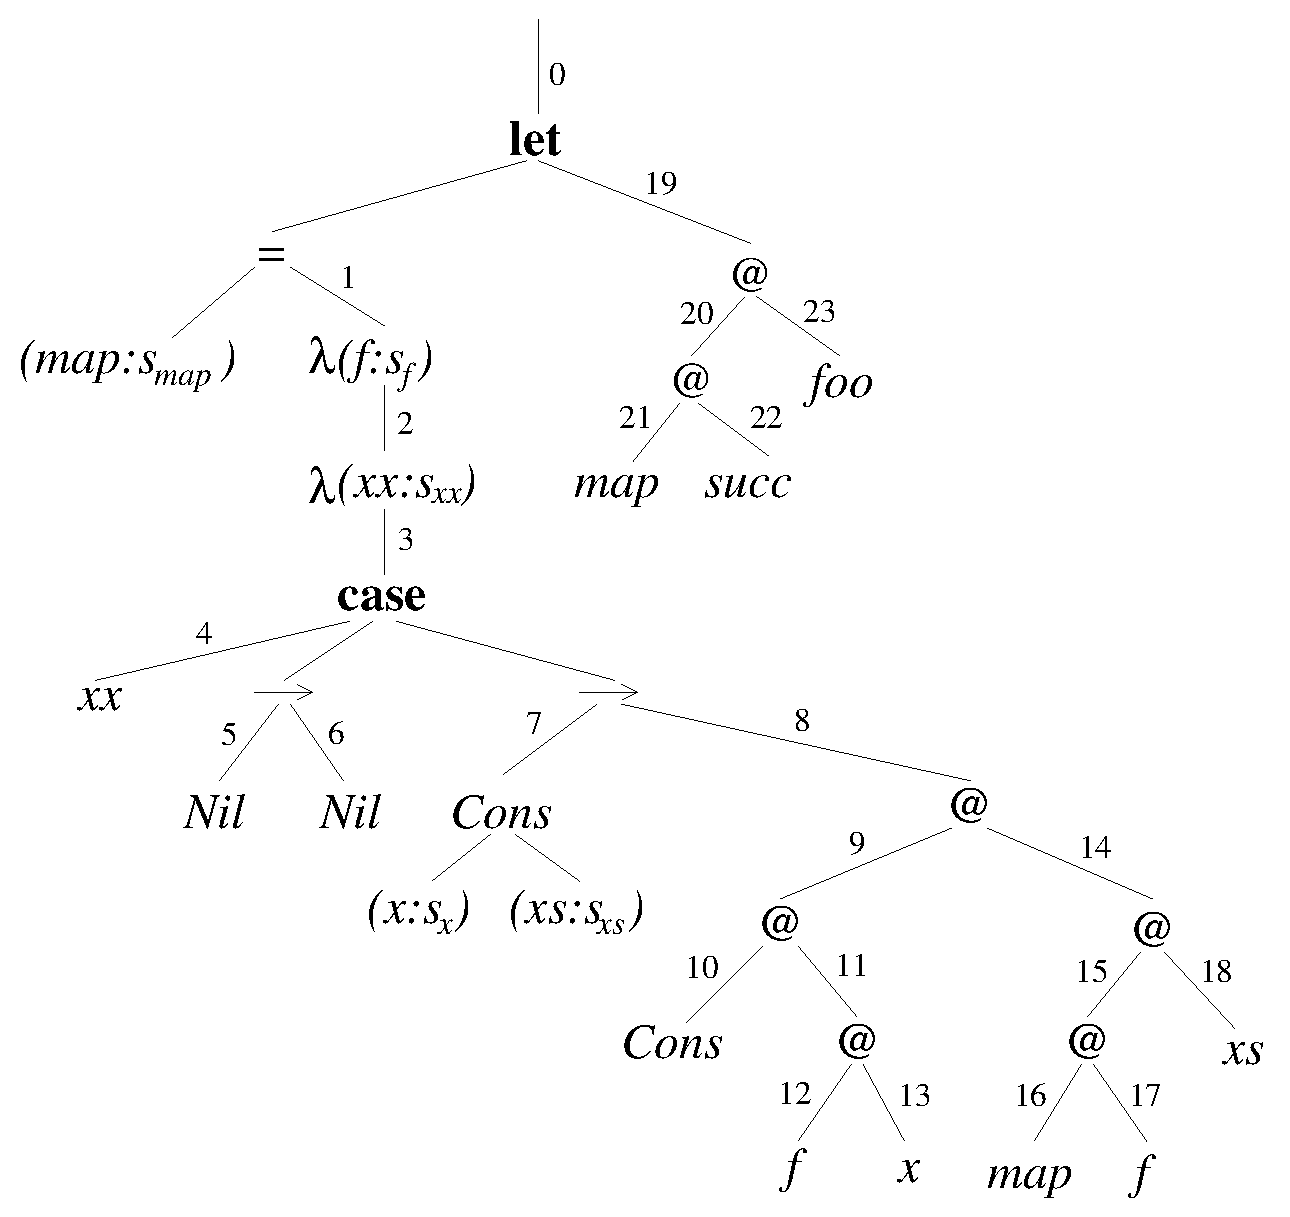
\includegraphics[scale=0.5]{3-Inference/fig/constraints/example-map}
\end{center}

\vspace{8em}
\code{
	$\klet$	& \mc{2}{$(\imap : s_{\imap}) = \lambda (f : s_f). \ \lambda (\ixx : s_{\ixx}).$} \\
		& \ \ $\kcase \ xx \ \kof$							\\
		& \ \ \ \ $\iNil$		& $\to \iNil$					\\
		& \ \ \ \ $\iCons \ (x : s_x) \ (\ixs : s_{\ixs})$
						& $\to \iCons \ (f \ x) \ (\imap \ f \ \ixs)$	\\
	$\kin$	& $\imap \ \isucc \ \ifoo$
}

\clearpage{}
\subsection{Slurping and constraint trees}
\label{Inference:Language:slurping}
In DDC we call the process of extracting type constraints from the annotated syntax tree \emph{slurping} the tree. The function $\rbSLURP$ takes this syntax tree and produces the corresponding constraint tree:

$$
\rbSLURP : \iSyntaxTree \to \iConstraintTree
$$

If the syntax tree has already been annotated with type variables and edge numbers, then the constraints for each node can be produced independently. However, in our implementation we prefer to annotate the tree and generate constraints in a single, bottom-up pass. 

The type constraints extracted from the program's syntax tree are represented by another tree that mirrors its overall shape. We use $\phi$ to represent a branch in this tree, and the branches have the following structure:

\vspace{-1ex}
\begin{tabbing}
MM	\= MM 	\= MM \= MMMMMMMMMMMMMMM \= MMMMMMM \kill
	\> $\phi$ 	\> $\to$ 	\> $\trm{INST} \ x$			
		\> (instantiate this var)		
		\\
\>	\> \ $\mid$	\> $\trm{LAMBDA} \ \ \ov{x} \ \	\ov{\phi}$	
		\> (lambda or case bound var) 		
		\\
\>	\> \ $\mid$	\> $\trm{LET} \ x \ \ 		\ov{\phi}$	
		\> (let bound var) 			
		\\
\>	\> \ $\mid$	\> $\trm{GROUP} \ \ov{x} \ \ 	\ov{\phi}$	
		\> (group of let bindings) 		
		\\
\>	\> \ $\mid$	\> $a = \varphi$
		\> (type equality)			
		\\
\>	\> \ $\mid$	\> $a \tme \varphi$
		\> (effect or closure inequality)
\end{tabbing}

$\rINST \ x$ corresponds to an occurrence of a bound variable in the program source. When extracting constraints we generate an $\rINST \ x$ for every occurrence, irrespective of whether the variable was bound by a let binding, lambda abstraction or pattern match. $\trm{LAMBDA} \ \ov{x} \ \ov{\phi}$ contains constraints arising from a lambda abstraction or pattern match. $\ov{x}$ is the list of bound variables and $\ov{\phi}$ is a list of constraint branches from the body of the abstraction. $\trm{LET} \ x \ \ov{\phi}$ contains constraints arising from a let binding. $\trm{GROUP} \ \ov{x} \ \ov{\phi}$ contains all the constraint branches from a particular mutually recursive let expression. $a = \varphi$ and $a \tme \varphi$ are individual constraints on type variables.

\clearpage{}
% -----------------------------------------------------------------------------
\subsection{Types of programs and declarations}
\label{inference:language:declarations}

\ruleBox{
	\begin{center}
	\fbox{$\Gamma \judge \ipgm :: \varphi$}
	\end{center}
	\begin{gather}
	\ruleI	{Pgm}
		{ \ov{\Gamma \judge \idecl :: \Gamma_d} \quad
		  \Gamma \judge t :: \varphi \quad
		  \Gamma = \Gamma_o, \ov{\Gamma_d}
		}
		{ \Gamma_o \judge \ov{\idecl} \ ; \ t :: \varphi }
	\end{gather}
}
\bigskip
\bigskip

\ruleBox{
	\begin{center}
	\fbox{$\Gamma \judge \idecl :: \Gamma'$}
	\end{center}
	\begin{gather}
	\ruleI	{DeclData}
		{ \ov{\trm{ValidCtor}(T, \ \% \to \ov{\kappa} \to *, \ \varphi)}}
		{ \Gamma \judge 
			\kdata \ T : \% \to \ov{\kappa} \to *  \ 
			\kwhere \ \ov{K : \varphi} \ 
				:: \ (T : \% \to \ov{\kappa} \to *, \ \ov{K : \varphi}) }
	\end{gather}
}

\bigskip
\code{
	\mc{2}{$\trm{ValidCtor}( T, \ \% \to \ov{\kappa} \to *, \ \varphi)$} \\
	 \qq \trm{where}
		& $\varphi = \forall (r : \%) \ \ov{a : \kappa}. \ T \ r \ \ov{a}$
	\\[2ex]
	\mc{2}{$\trm{ValidCtor}( T, \ \% \to \ov{\kappa} \to *, \ \varphi)$} \\
	 \qq \trm{where}
		& $\varphi = \forall (r : \%) \ \ov{a : \kappa}. \ \tau \to T \ r \ \ov{a}$ \\
		& $\ifv(\tau) \setminus \{ r, \  \ov{a} \} \subseteq \emptyset$
	\\[2ex]
	\mc{2}{$\trm{ValidCtor}( T, \ \% \to \ov{\kappa} \to *, \ \varphi)$} \\
	 \qq \trm{where}
		& $\varphi = \forall (r : \%) \ \ov{a : \kappa} \ (c : \$). 
			\ \tau_1 \to \tau_2 \lfuna{c}T \ r \ \ov{a} \ \rhd c \tme x_1 : \tau_1$ \\
		& $(\ifv(\tau_1) \cup \ifv(\tau_2)) \setminus \{ r, \  \ov{a} \} \subseteq \emptyset$
}

\bigskip
In (Pgm), we set the overall type of the program to be the type of its final expression. As data type declarations can be mutually recursive, we add the types and kinds generated by each one to the type environment used when checking them.

In (DeclData) the predicate ValidCtor checks that each constructor has a type appropriate to the data type being declared. We have given the first few cases of ValidCtor, and leave the inductive generalisation to the reader. In our implementation we \emph{generate} the types of data constructors from Haskell style algebraic type definitions, instead of requiring the programmer to give them explicitly, but the checking rules are easier to present.
 
The definition of ValidCtor has several points of note: the type of a constructor cannot have free variables; the type of the return value must have a primary region variable; the types of parameters cannot contain variables that are not present in the return type, and constructors do not have side effects. Also note that the function arrows of constructor types must have appropriate closure annotations, the last case of ValidCtor is an example. This is needed to support the partial application of data constructors.

% -----------------------------------------------------------------------------
\subsection{Kinds of types and constraints}

\ruleBox{
	\begin{center}
	\fbox{ $\varphi :: \kappa$ }
	\end{center}
	\vspace{-1em}
	\begin{gather}
	\ruleA	{KiVar}
		{ a_\kappa :: \kappa }
	\ruleSkip
	\ruleI	{KiConstr}
		{ \varphi :: \kappa \quad
		  \ov{\chi :: \kappa'} \quad
		  \chi \in \Omega
		}
		{ \varphi \rhd \Omega :: \kappa }
	\ruleSkip
	\ruleI	{KiAll}
		{ \varphi :: \kappa' }
		{ \forall(a_{\kappa} : \kappa). \ \varphi :: \kappa' }
	\ruleSkip
	\ruleI	{KiJoin}
		{ \varphi_1 :: \kappa \quad
		  \varphi_2 :: \kappa \quad
		  \kappa \in \{ \ !, \ \$ \ \} 
		}
		{ \varphi_1 \lor \varphi_2 :: \kappa }
	\ruleSkip
	\ruleI	{KiBot}
		{ \kappa \in \{ \ !, \ \$ \ \} }
		{ \bot_{\kappa} :: \kappa }
	\ruleSkip
	\ruleA	{KiTop}
		{ \top_{!} :: \ ! }
	\ruleSkip
	\ruleI	{KiFun}
		{ \tau_1    :: * \quad
		  \tau_2    :: * \quad
		  \sigma    :: \ ! \quad
		  \varsigma :: \$ 
		}
		{ \tau_1 \lfuna{\sigma \ \varsigma} \tau_2 :: * }
	\ruleSkip
	\ruleI	{KiData}
		{ r :: \% \quad
		  \ov{\varphi :: \kappa}
		}
		{ T_{\% \to \ov{\kappa} \to *} \ \ r \ \ \ov{\varphi} :: *}
	\ruleSkip
	\ruleI	{KiRead}
		{ r :: \% }
		{ \iRead \ r :: \ ! }
	\ruleSkip
	\ruleI	{KiReadH}
		{ \varphi :: * }
		{ \iReadH \ \varphi :: \ ! }
	\ruleSkip
	\ruleI	{KiWrite}
		{ r :: \% }
		{ \iWrite \ r :: \ ! }
	\ruleSkip
	\ruleI	{ KiClo }
		{ \varphi :: \kappa \quad
		  \kappa \in \{ \ *, \ \$ \ \} }
		{ (x : \varphi) :: \$ }
	\end{gather}
}

\bigskip
\ruleBox{
	\begin{center}
	\fbox{ $\chi :: \kappa$ }
	\end{center}
	\vspace{-1em}
	\begin{gather}
	\ruleI	{KiCEq}
		{ \tau_1 :: \kappa \quad \tau_2 :: \kappa}
		{ (\tau_1 = \tau_2) :: \kappa }
	\ruleSkip
		\ruleI	{KiCGeq}
		{ \varphi_1 :: \kappa 
		  \quad
		  \varphi_2 :: \kappa 
		  \quad
		  \kappa \in \{ \ !, \ \$ \ \} }
		{ (\varphi_1 \tme \varphi_2) :: \kappa }
	\end{gather}
}

\clearpage{}
Our kinding rules are mostly standard. In (KiConstr) we use the term $\ov{\chi :: \kappa'}$ to require each of the constraints to have a valid kind. The $\chi :: \kappa$ \ judgement ensures that the types on both sides of a constraint have the same kind.


% -----------------------------------------------------------------------------
\subsection{Types of terms}
\begin{center}
	\fbox{$\Gamma \judge t :: \varphi \rhd \Omega \ ; \ \sigma$}
\end{center}


The judgement form $\Gamma \vdash t :: \varphi \ \rhd \ \Omega \ ; \sigma$ reads: ``with environment $\Gamma$ the term $t$ has type $\varphi$, constraints $\Omega$ and effect $\sigma$.'' We will assume that $\varphi$ contains no further constraint sets, and that the typing rules maintain this property. This is a slight abuse of $\rhd$, but we find it more convenient than introducing another operator. Our handling of constraints is based on Leroy's closure typing system \cite{leroy:polymorphic-type-inference}, so the constraint set $\Omega$ is global. When building a type scheme we will include only the constraints reachable from the body of the type. Leroy's approach can be contrasted with Jones's system of qualified types \cite{jones:qualified-types} which encodes constraints as bounds on quantifiers, and uses separate rules to move them between local types and the global set. Our core language uses this second system instead, and we convert between the two representations when translating the source program to core.

In our typing rules we make no attempt to keep the constraint set consistent or satisfiable. Inconsistencies such as $\iInt \ r \ \rhd \iMutable \ r, \ \iConst \ r$ or $\bot \tme \iConsole$ will be discovered when the program is converted to core. The core typing rules ensure that witnesses to the mutability and constancy of a particular region cannot exist in the same program, and effect constraints are checked during type application. Attempting to translate a program that includes inconsistent type constraints to the core language will result in a core type error. However, if these problems are instead detected during type inference, then the compiler would be in a better position to emit a helpful error message. Error handling is discussed in \S\ref{inference:errors}.

The typing rules are presented in three parts, with the static rule in the center, the associated node of the abstract syntax tree on the left, and the generated type constraints on the right. The combination of node and type constraints inductively defines the $\rbSLURP$ function mentioned in \S\ref{Inference:Language:slurping}.

\clearpage{}
% -----
\textbf{Var / Ctor}
$$
\begin{aligned}
	\frac	{x : \forall \ov{a : \kappa}. \ \varphi \rhd \Omega \in \Gamma}
		{\Gamma \judge x :: \varphi[\ov{\varphi'/a}] 
					\rhd \Omega[\ov{\varphi'/a}] \cup \Omega' \ ; \ \bot}
\end{aligned}
$$

\begin{tabbing}
MMMMMMMMMMMMMMMMMMMMM \= MMMMMMMMMMMMM \kill
	\hspace{10em}\includegraphics[scale=0.6]{3-Inference/fig/constraints/var}	
	\> 
	\begin{tabular}{ll}
		$s_1$ 	& $= \rINST \ s_x$ \\
		\\
       	\end{tabular}
\end{tabbing}

We assume that the source program's syntax has already been checked, so $x$ is bound somewhere above its use. The rule for data constructors is identical to the one above, with $x$ replaced by $K$.

The type for $x$ is required to be in the environment, and this type may include quantifiers $\forall \ov{a : \kappa}$ and more constraints $\Omega$. We instantiate this type scheme by substituting new types $\ov{b}$ for the quantified variables in the body of the type as well as its constraints. The extra constraint term $\Omega'$ is needed to match the constraints introduced by other parts of the program, and allows the instantiated type to be weakened and treated as having a larger effect or closure term than it does in the environment. This is required when typing the higher order examples discussed in \S\ref{System:Effects:constraint-strengthening}.

When generating constraints we defer the question of whether the variable was introduced by a let binding, lambda binding, pattern match, or whether it is part of a (mutually) recursive group. If a variable turns out to have been bound by a lambda or pattern match there will be no corresponding generalisation of its type, but we will use $\rINST$ to instantiate it anyway. This makes the resulting constraints easier to read, and simplifies discussion of how to work out the binding dependency graph in \S\ref{inference:ordering}. During type inference we can think of $\rINST$ as a function that blocks on the variable $s_x$, waiting for the type scheme of $x$ to be become available.

\bigskip
% -----
\textbf{Abs}
$$
\begin{aligned}
	& \frac
		{\Gamma, \ x : \tau_1 \rhd \Omega_1 \judge t_2 :: \tau_2 \rhd \Omega_2 \ ; \ \sigma_2}
		{\Gamma \judge \lambda x. \ t_2 \ 
				:: \  \tau_1 \lfuna{e_2 \ c_1} \tau_2 \rhd \Omega_1 \cup \Omega_2 ; \ \bot}
	\\[1ex]
	& \trm{where} \ \ 	\trm{for all} \ y \in \ifv(\lambda x. \ t_2) 
					\ \trm{we have} \ (c_1 \tme y : \Gamma(y)) \in \Omega_2 \\
	& \hspace{7.5ex}	\trm{and} \ e_2 \tme \sigma_2 \in \Omega_2 
\end{aligned}
$$

\begin{tabbing}
MMMMMMMMMMMMMMMMMMM \= MMMMMMMMMMMMM \kill
	\hspace{8em}\includegraphics[scale=0.5]{3-Inference/fig/constraints/lam}
	\> 
	\begin{tabular}{llll}
		\mc{4}{LAMBDA \ $\{ x \}$} \\
			& $s_1$ 	& $= s_x \lfuna{e_2 \ c_1} s_2$ \\
			& $c_1$		& $\tme y_0 : s_{\iyZero} \ \lor \ y_1 : s_{\iyOne} \ \lor \dots$ \\
			&		& $\ \ \ \ \trm{where} \ y_n \gets \ifv(\lambda x. \ t_2)$ 
			\\[1ex]
			& \mc{2}{$\rbSLURP (t_2)$}
		\\ \\ \\ \\
	\end{tabular}
\end{tabbing}

\vspace{-4em}
An abstraction takes a term of type $\tau_1$ and produces a term of type $\tau_2$. When the abstraction is applied it will have the effect $\sigma_2$ of its body. In the typing rule we give this effect the name $e_2$ and bind it to $\sigma_2$ in $\Omega_2$. When generating constraints we can simply annotate the function constructor with $e_2$, and the required effect constraints will be generated when slurping the body. As evaluating the abstraction itself causes no effect, we have $\bot$ in the conclusion of the rule.

The closure of an abstraction contains the types of its free variables. In the typing rule we can read these types directly from the environment using $\Gamma(y)$. When we're generating constraints we won't know what these types are yet, so we use the the place holder variables $s_{\iyZero}, s_{\iyOne} ...$ instead. These variables will be bound to their real types during inference.

\bigskip
% -- App -------------
\textbf{App}

$$
\begin{aligned}
	\frac	{\begin{aligned}
			\Gamma & \judge t_2 :: \tau_3 \lfuna{\sigma_4 \ \varsigma_4} \tau_1 \rhd \Omega
					; \ \sigma_2  \\
			\Gamma & \judge t_3 :: \tau_3 \rhd \Omega \ ; \ \sigma_3 
		 \end{aligned}
		}
		{ \begin{aligned}
		  	\Gamma & \judge t_2 \ t_3 :: \tau_1 \rhd \Omega \ ; \ \sigma_2 \lor \sigma_3 \lor \sigma_4
		  \end{aligned}
		}
\end{aligned}
$$

\begin{tabbing}
MMMMMMMMMMMMMMMMMMMMM \= MMMMMMMMMMMMM \kill
	\hspace{8em}\includegraphics[scale=0.5]{3-Inference/fig/constraints/app}
	\>
	\begin{tabular}{llll}
		$s_2$	& $=	s_3 \lfuna{e_4 \ c_4} s_1$	\\
		$e_1$	& $\tme	e_2 \lor e_3 \lor e_4$ \\[1ex]
		\mc{2}{$e_4, \ c_4$ \trm{fresh}} \\
		\mc{2}{$\rbSLURP(t_2)$} \\
		\mc{2}{$\rbSLURP(t_3)$} \\
		\\ \\ \\ \\
	\end{tabular}
\end{tabbing}

\vspace{-5em}
An application node applies a function of type $\tau_3 \lfuna{\sigma_4 \ \varsigma_4} \tau_1$ to its argument of type $\tau_3$, yielding a result of type $\tau_1$. The act of applying the function has an effect $\sigma_4$. The effect of evaluating the entire expression consists of the effect of evaluating the function value, of evaluating the argument, and of applying the function. In the terminology of \cite{lucassen:polymorphic-effect-systems}, $\sigma_4$ is the \emph{intrinsic} effect of the application and $\sigma_2 \lor \sigma_3$ is the \emph{inherited} effect. The closure of the function is of no consequence when typing an application, so $\varsigma_4$ is only mentioned once in the rule.

When generating type constraints we will not yet know what the effect of the function will be. In our constraints we use $e_4$ and $c_4$ as local names for the function's effect and closure. These will be bound to the actual effect and closure of the function during type inference.

\clearpage{}
% -----
\textbf{Let-Poly}

$$
\begin{aligned}
	\frac	{\begin{aligned}
			\Gamma, \ \ov{x_n : \varphi_n} &  \judge t :: \tau \rhd \Omega \ ; \ \sigma 
			\\
			\Gamma, \ \ov{x_n : \tau_n \rhd \Omega}  
					&  \judge t_0' :: \tau_0' \rhd \Omega \ ; \ \sigma_0'
			\qq \varphi_0 = \rGen(\Gamma, \ \tau_0' \rhd \Omega)
			\\
			\Gamma, \ \ov{x_n : \tau_n \rhd \Omega}  
					&  \judge t_1' :: \tau_1' \rhd \Omega \ ; \ \sigma_1'
			\qq \varphi_1 = \rGen(\Gamma, \ \tau_1' \rhd \Omega) 
			\\
			& \ \vdots \hspace{10em}\ \hspace{4em} \vdots
		 \end{aligned}}
		{\begin{aligned}
			\Gamma & \judge \klet \ \ov{x_n = t_{n}'} \ 	
				\kin \ t :: \tau \rhd \Omega \ ; \ \sigma \lor \sigma_0' \lor \sigma_1' \lor \dots
		 \end{aligned}}
 \end{aligned}
$$

\bigskip
\begin{tabbing}
MMMMMMMMMMMMMMMMMMMMMMM \= MMMMMMMMMMMMM \kill
	\ \ \ \ 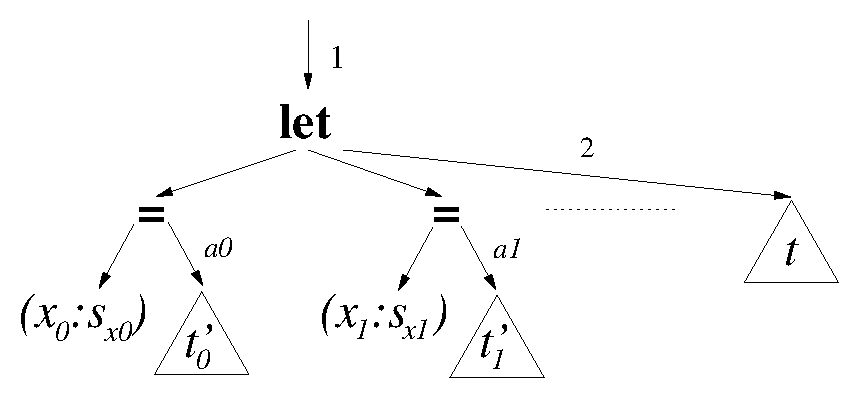
\includegraphics[scale=0.5]{3-Inference/fig/constraints/let}
	\> 
	\begin{tabular}{llll}
		\mc{4}{GROUP $\{ x_0, \ x_1,  \ \dots \}$} \\
			& \mc{3}{$s_1 = s_2$} \\
			& \mc{3}{$e_1 \tme e_{a0} \lor e_{a1} \lor \dots \lor e_2$} 
			\\[1ex]
			& \mc{3}{LET $x_0$} \\	
			&	& $s_{x0} = s_{a0} $ \\
			&	& \textbf{SLURP}($t_0'$) 	\\
			& \mc{3}{LET $x_1$} \\	
			&	& $s_{x1} = s_{a1} $ \\
			&	& \textbf{SLURP}($t_1'$) 	\\
			& \ \ \vdots \\
			& \mc{2}{\textbf{SLURP}($t$)}
 	\end{tabular}
\end{tabbing}

The function Gen generalises the types of each binding. This process is discussed in \S\ref{inference:generalisation}. Note that in the expression:

\code{
	$\varphi = \rGen(\Gamma, \ \tau \ \rhd \Omega)$
}

The resulting type $\varphi$ contains only the constraints from $\Omega$ that are reachable from $\tau$. The conclusion of (Let-Poly) includes the constraint set $\Omega$, and the same set is used in each of the premises. This means that constraints that are conceptually local to a particular binding will ``leak'' into the global set. For example:

$$
	\frac	
	{\begin{aligned}
	 & \Gamma, \ \isuccL : \forall r_1 \ r_2. \ \iInt \ r_1 \to \iInt \ r_2 \rhd \iConst \ r_1 \\
	 & \qq \judge \isuccL \ 3 \\
	 & \qq \ :: \ \iInt \ r_3 \ \rhd \  \iConst \ r_3, \ \iConst \ r_4 \ ; \ \bot
	 \\[1ex]
         & \Gamma, \ \isuccL : \iInt \ r_4 \to \iInt \ r_5 \rhd \iConst \ r_3, \ \iConst \ r_4 \\
	 & \qq \judge \lambda x. \ \isuspendOne \ \isucc \ x  \\
	 & \qq \ :: \ \iInt \ r_4 \to \iInt \ r_5 \rhd \iConst \ r_3, \ \iConst \ r_4 \ ; \ \bot \\[1ex]
	 \end{aligned}
	}
	{\begin{aligned}
	 \Gamma & \judge \klet \ \isuccL = \lambda x. \ \isuspendOne \ \isucc \ 
x \ \kin \ \isuccL \ 3 \\
	 & \ :: \ \iInt \ r_3 \rhd \iConst \ r_3, \iConst \ r_4 \ ; \ \bot
	 \end{aligned}
	}
$$

The function $\isuccL$ is a lazy version of $\isucc$ that reads its argument only when the result is demanded. The general type of $\isuccL$ is:

\code{
	$\isuccL :: \forall r_1 \ r_2. \ \iInt \ r_1 \to \iInt \ r_2 \rhd \iConst \ r_1$
} 

The constraint $\iConst \ r_1$ arises from the use of $\isuspendOne$ in the definition of $\isuccL$. When checking this definition we give $\isuccL$ the monotype:

\code{
	$\iInt \ r_4 \to \iInt \ r_5 \rhd \iConst \ r_4$
}

Due to the formulation of the (Let-Poly) rule, the constraint $\iConst \ r_4$ is actually present in \emph{both} premises, as well as the conclusion. Also, in the body of the let-expression, the application of $\isuccL$ to the constant $3$ requires that constant to be (really) constant, hence the constraint $\iConst \ r_3$. Although this constraint only concerns the body of the let-expression, it is also present in the set used when typing the bindings.

This behavior is unlike that of the (Let) rule presented by Leroy in \cite{leroy:polymorphic-type-inference}. Leroy's rule uses $\rGen$ to split the constraint set arising from a let-binding into two subsets: those that are reachable from the body of the type being generalised, and those that aren't. If we were to use Leroy's approach, the first premise and conclusion of our example would not contain $\iConst \ r_4$, and the second premise would not contain $\iConst \ r_3$. Leroy's rule is ``nicer'' when drawing proof trees, but we stick to the leaky version because it mirrors what happens during type inference. Our inference algorithm adds all the type constraints extracted from the program into a global graph, solves them, then returns the whole graph. It does not section the graph into portions relating to individual bindings, and it only removes constraints from the graph when dealing with the type classes discussed in \S\ref{inference:type-classes}. Retaining information from all bindings also makes it easy for the implementation to add type annotations to the desugared program when converting it to core.

As we have not implemented polymorphic recursion \cite{mycroft:polymorphic-recursion}, we check the right of each binding using the ungeneralised types for each let-bound variable. Due to this, many useful programs are not directly typeable with this (Let-Poly) rule. Consider this example from \cite{mycroft:polymorphic-recursion}:

\bigskip
\qq\qq
\begin{tabular}{lll}
	$\klet$	& \mc{2}{$\imap = \lambda f. \ \lambda \ixx.$}					\\
		& \ \ $\kcase \ xx \ \kof$							\\
		& \ \ \ \ $\iNil$		& $\to \iNil$					\\
		& \ \ \ \ $\iCons \ x \ \ixs$	& $\to \iCons \ (f \ x) \ (\imap \ f \ \ixs)$	
		\\[1ex]
		& $\isquarelist$ & \hspace{-2em} $= \lambda l. \imap \ (\lambda x. \ x * x) \ l$
		\\[1ex]
		& $\icomplement$ & \hspace{-2em} $= \lambda l. \imap \ (\lambda x. \inot x) \ l$
		\\[1ex]
	$\kin$	& \dots
\end{tabular}
\bigskip

This program will not be accepted as it stands. We need to use the generalised, polymorphic type of map when applying it to $(\lambda x. \ x * x)$ and $(\lambda x. \inot x)$ because these expressions have different types. If we use the ungeneralised, monomorphic type then we will get an error.

This highlights the fact that our source typing rules are only a guide for generating type constraints, and that we cannot use them to check the source program directly. We must first perform type inference by extracting type constraints and then solving them. As discussed in \S\ref{inference:ordering}, our algorithm for solving type constraints also builds a graph that records what bindings are mutually recursive. Once we have this graph we can use it to split out the definition of $\imap$ from the above example, and convert the program to:

\bigskip
\qq\qq
\begin{tabular}{lll}
	$\klet$	& \mc{2}{$\imap = \lambda f. \ \lambda \ixx.$}					\\
		& \ \ $\kcase \ xx \ \kof$							\\
		& \ \ \ \ $\iNil$		& $\to \iNil$					\\
		& \ \ \ \ $\iCons \ x \ \ixs$	& $\to \iCons \ (f \ x) \ (\imap \ f \ \ixs)$	
		\\[1ex]
	$\kin$ \\
	$\klet$	& $\isquarelist$ & \hspace{-2em} $= \lambda l. \imap \ (\lambda x. \ x * x) \ l$
		\\[1ex]
		& $\icomplement$ & \hspace{-2em} $= \lambda l. \imap \ (\lambda x. \inot x) \ l$
		\\[1ex]
	$\kin$	& \dots
\end{tabular}

\bigskip
For this version, (Let-Poly) allows us to use the generalised type of $\imap$ when checking the body of the second let-expression. This new program will be accepted without error.

% The effect of the whole expression includes the effects $\sigma_0, \sigma_1, \dots$ of its bindings along with the effect $\sigma$ of the body. The structure of the constraints mirrors that of the original expression. \trm{GROUP} signals that the enclosed constraints contain a refer to a set of (mutually) recursive $\klet$ bindings, and \trm{LET} denotes the scope of each one. 

\bigskip
% ----------
\textbf{Case}
$$
\begin{aligned}
	\frac	
	{\begin{aligned}
		\begin{aligned}
		  \\ \\ \\
		  \Gamma & \judge t :: T \ r \ \ov{\varphi} \rhd \Omega \ ; \ \sigma 
		\end{aligned}
		&
		\begin{aligned}
		  \Gamma & \judgea{p} p_0 \to t_0' :: T \ r \ \ov{\varphi} \to \tau \rhd \Omega \ ; \ \sigma_0' \\
		  \Gamma & \judgea{p} p_1 \to t_1' :: T \ r \ \ov{\varphi} \to \tau \rhd \Omega \ ; \ \sigma_1' \\
		 	 & \hspace{6em} \vdots
	 	\end{aligned}
	 \end{aligned} 
	}
	{\begin{aligned}
	  \Gamma  & \judge \kcase \ t \ \kof \ \ov{p \to t'} :: \tau' \rhd \Omega
				\ ; \ \iRead \ r \lor \sigma \ \lor \sigma_0' \lor \sigma_1' \lor \dots
	 \end{aligned}
	}
 \end{aligned}
$$

\begin{tabbing}
	MMMMMMMMMMMMMMMMMMM \= MMMMMMMMMMMMM \kill
	\hspace{1em}\includegraphics[scale=0.5]{3-Inference/fig/constraints/case} 
	\> \begin{tabular}{lll}
		$s_2$ 	& $= s_{p0}$ \\
		$s_2$	& $= s_{p1}$ \\
			& \ \ \vdots \\
		$s_1$	& $= s_{a0}$ \\
		$s_1$	& $= s_{a1}$ \\
			& \ \ \vdots \\
		$e_1$	& $= \iReadH s_2 \lor e_2 \lor e_{a0} \lor e_{a1} \lor \dots$ \\
		\mc{2}{$\rbSLURP(t)$} \\
		\mc{2}{$\rbSLURP(p_0)$} \\
		\mc{2}{$\rbSLURP(p_1)$} \\
			& \ \ \vdots \\
		\mc{2}{$\rbSLURP(t_0)$} \\
		\mc{2}{$\rbSLURP(t_1)$} \\
			& \ \ \vdots \\
		\\ \\ \\ \\ \\ \\ 
	    \end{tabular}
\end{tabbing}

\vspace{-8em}

A case expression requires the discriminant $t$ to have the same type as the patterns being matched against. For all alternatives, the types of the patterns must be identical, and so must the types of the expressions. The type of the entire case expression is the type of the right of the alternatives. 

The effect of a case expression includes the effect of evaluating the discriminant and examining it, as well as evaluating the alternatives. When type checking a program in a bottom-up manner, when it's time to apply the (Case) rule we will already know the type of the discriminant. In this situation we can use $\iRead \ r$ as the effect of examining it. On the other hand, when generating constraints we will not yet know the type of the discriminant. We instead use $\iReadH s_2$, which represents a read effect on the primary region of the (currently unknown) type $s_2$. During inference, the type of $s_2$ will resolve to the real type of the discriminant. After this is done, $\iReadH s_2$ can be reduced to a $\iRead$ effect on the primary region of this new type.

\clearpage{}
\ruleBox{
	\begin{center}
	\fbox{ $\Gamma \judgea{p} p \to t :: \tau_1 \to \tau_2 \rhd \Omega$ }
	\end{center}
	\vspace{-1em}
	\begin{gather}
	\ruleI	{Pat-Wildcard}
		{ \Gamma \judge t :: \tau_2 \rhd \Omega \ ; \ \sigma }
		{ \Gamma \judgea{p} \_ \to t :: \tau_1 \to \tau_2 \rhd \Omega \ ; \ \sigma }
	\ruleSkip
	\ruleI	{Pat-Constructor}
		{ 	T & : \% \to \ov{\kappa} \to * \in \Gamma
			\\
			K & : \forall (r : \%) \ \ov{a : \kappa} \ \ov{c : \$}
				. \ \ov{\tau} \lfuna{c'} T \ r \ \ov{a} \ \rhd \Omega \in \Gamma 
			\qq \theta = [\ r' / r \ \ \ov{\varphi/a} \ ]
			\\
	  		& \Gamma, \ \ov{x_n : \theta(\tau_n) \ \rhd \ \theta(\Omega)}^{\: n}
				\judge t :: \tau' \rhd \Omega' \ ; \ \sigma
		}
		{ \Gamma \judgea{p} K \ \ov{x} \to t 
			:: T \ r' \ \ov{\varphi} \to \tau' \rhd \Omega' \ ; \sigma }
	\end{gather}
}
\bigskip
\begin{tabbing}
	MMMMMMMMMMMMMMMMM \= MMMMMMMMMMMMM \kill
	\hspace{6em}\includegraphics[scale=0.5]{3-Inference/fig/constraints/pat} 
	\> $\begin{aligned}
		s_1 & = T \ r' \ \ov{a'} \\
		s_x & = \tau' \\
		\vdots \\
                & \trm{where} \ \tau' \to \dots \to T \ r' \ \ov{a'}\\
		& \hspace{2em}  = \trm{Inst}(\forall (r : \%) \ \ov{a : \kappa} \ \ov{c : \$}
					. \ \ov{\tau} \lfuna{c'} T \ r \ \ov{a})
		\\ \\ \\
	    \end{aligned}$
\end{tabbing}

\vspace{-2em}
The judgement form $\Gamma \judgea{p} p \to t :: \tau_1 \to \tau_2 \rhd \Omega$ reads: ``with environment $\Gamma$ an alternative matching a pattern $p$ and producing a term $t$ has type $\tau_1$ to $\tau_2$ with constraints $\Omega$.''

Matching against a wildcard produces no constraints.

In (Pat-Constructor) we lookup the type of the constructor $K$ from the environment. The (DeclData) rule from \S\ref{inference:language:declarations} introduces these types into the environment and ensures that they have the particular form shown here.

The variables bound by the pattern are named $\ov{x}$, and the types of these variables must have the same form as the types of the arguments of the constructor. If the constructor produces a type containing variables $\ov{a}$ then all occurrences of $\ov{x}$ must agree on the particular types used for $\ov{a}$. For example with the constructor:

\code{
	$\iCons :: \forall r \ a \ c. \ a \to \iList \ r \ a \lfuna{c} \iList \ r \ a \ \rhd \ c \tme x : a$
}

Consider the alternative in:

\code{
	$\kcase \ \dots \ \kof$ \\
	\ \ $\iCons \ x \ \ixs \to \dots$
}

We cannot, say, use $x$ at type $\iInt \ r_1$, but $\ixs$ at type $\iCons \ r_2 \ (\iBool \ r_1)$ because $\iInt \ r_1 \ \neq \ \iBool \ r_1$. This restriction is achieved by requiring the types of each of the pattern bound variables to be related by the substitution $\theta$.

The constraint generation rules given here only concern the pattern in a particular alternative. The job of matching up the types of all alternatives in a case-expression is handled by the constraints for the (Case) rule on the previous page. 

When generating constraints for a pattern, we first take a fresh instance of the constructor's type scheme. The result type is the type of the overall pattern, and the argument types are assigned to the variables bound by the pattern.






\smallskip
% -------------------------------------
\noindent
\textbf{Kinds}\\
A kind can be a constructor $\kcData$, $\kcRegion$ or $\kcEffect$. These are the primitive kinds of data types, region types and effect types respectively. We use $(\kto)$ as the function kind constructor, using a different arrow symbol to distinguish it from the type constructor $(\to)$. 


\smallskip
% -------------------------------------
\noindent
\textbf{Types}\\
Type variables are written $ix\bra{a}$, where $ix$ is the de Bruijn index and $\bra{a}$ is a suggestive variable name. In all cases, if the reader prefers the concrete de Bruijn representation for binders, then they can simply erase the names between $\bra{}$ braces. 

We join effect types with ~$\mtype + \mtype$, and the kinding rules in Fig.~\ref{f:KindT} constrain both type arguments to have the $\kcEffect$ kind. The effect of a pure computation is written $\bot$. 

The type $\mtycon_n$ is a primitive type constructor of arity $n$. To simplify the presentation, all type constructors except $(\to)$ must be fully applied. In a larger language, partial application of the other constructors could be encoded using type synonyms.

The type $\trgn{p}$ is a region handle which contains a natural number $p$ that identifies a runtime region.  A region handle is a \emph{static capability}, whose existence in a well typed expression indicates that region $p$ currently exists; can have new store bindings allocated into it, and can be read from and written to. Region handles are similar to the capabilities of \cite{Walker:static-capabilities}, except that they appear directly in the type language rather than being present in a separate environment of the typing judgment. Region handles can also be captured in function closures and appear in functional values held in the store.


\eject
% -------------------------------------
\noindent
\textbf{Values and Expressions}\\
Values are the expressions that cannot be reduced further. Expression variables are written $ix\bra{z}$, where $ix$ is again a de Bruijn index and $\bra{z}$ a suggestive variable name. 

The value ~$\vloc{l}$~ is a store location that contains a natural number $l$ giving the address of a mutable reference. All store locations have type $\tcRef~ t_1~ t_2$, where $t_1$ is the region that location is in and $t_2$ is the type of the value at the location.

Function applications and primitive operators work on values rather than reducible expressions. As we will see in \S\ref{s:Dynamics}, this restriction ensures that the dynamic semantics only needs to deal with two reduction contexts, namely the right of a $\klet$ binding, and a context that includes a new region variable. The expression \mbox{$\xlet{\bra{z}}{t_1}{x_1}{x_2}$} first reduces $x_1$ to a value before substituting it for $z$ in $x_2$ (or for index \un{0} using the de Bruijn notation). 

The expression ~$\mop_n~ \ov{\mval}^{\; n}$~ is a fully applied, pure primitive operator, where $n$ is the arity of the operator. The pure operators do not affect the store. 

The expression ~$\xprivate{\bra{r}}{x}$~ creates a new region, then substitutes the corresponding region handle for variable $r$ in body $x$. It then reduces this new body to a value~$v$ and deallocates the region. The result of the overall expression is $v$. 

The expression ~$\xextend{t_1}{\bra{r_2}}{x}$~ takes the handle $t_1$ of an existing region, and creates a new region for $r_2$, which is available in body $x$. It then reduces $x$ to a value $v$. Once the reduction of $x$ has completed, all store bindings in the new region $r_2$ are merged into the original region with handle $t_1$. The result of the overall expression is $v$.

The expression $\xalloc{t}{v}$ takes a region handle $t$, a value $v$, and allocates a new store binding in that region containing the given value. The expression $\xread{t}{v}$ takes a region handle $t$, a store location $v$ in that region, and reads the value at the location. Finally, $\xwrite{t}{v_1}{v_2}$ takes a region handle $t$, a location $v_1$ in that region, a new value $v_2$, and overwrites the value in the store binding at location $v_1$ with the new value $v_2$.




%!TEX root = ../Main.tex

\section{Static Semantics}
%!TEX root = ../../Main.tex

% -----------------------------------------------------------------------------
Fig.~\ref{f:Environments} shows the environments we use in both the kinding rules of Fig.~\ref{f:KindT} and typing rules of Fig.~\ref{f:TypeX}. In the Coq formalization these are de Bruijn environments, indexed by number, starting from the \emph{right}. Following our hybrid presentation we also include suggestive variable names. We index environments from the right so that they appear as stacks that grow to the left. For example, consider the following kind environment:
$$
\bra{a_1} : \kcData,~~ \bra{e_1} : \kcEffect,~~ \bra{r_1} : \kcRegion
$$

Here, index $\un{0}$ refers to the element $\bra{r_1} : \kcRegion$ and index $\un{1}$ to $\bra{e_1} : \kcEffect$. For this reason we write the corresponding type variables as $\un{0}\bra{r_1}$ and $\un{1}\bra{e_1}$ respectively. In typing judgments we write an empty environment using a single $\cdot$ dot.

In Fig.~\ref{f:Environments}, the kind environment $\mkienv$ and type environment $\mtyenv$ consist of a list of kinds and types as usual. The store environment $\mstenv$ gives the type of each location in a store, and the store properties $\mstprops$ records the identifiers of regions that have been created so far. When a region is deallocated all the bindings in that region of the store are marked as dead. However, we retain the corresponding entry in the list of store properties so that any dangling references to those bindings are still well typed.


% -----------------------------------------------------------------------------
%!TEX root = ../Main.tex

\begin{figure}
\boxfig{

\begin{center}
\hspace{3em}
$\fbox{$\KindT{\mkienv}{\mstprops}{\mtype}{\mkind}$}~~ (\trm{KindT})$
\end{center}

% -------------------------------------
% | KiVar
%   :  forall ke sp i k
%   ,  get i ke = Some k
%   -> KindT ke sp (TVar i) k
$$
\ruleIL {KiVar}
{       \ck{k}  = \trm{get}~~ \ct{ix\bra{a}}~~ ke
}
{       \KindT  {\mke}{\msp}
                {ix\bra{a}}
                {k}
}
\qq
% -------------------------------------
% | KiRgn
%   :  forall ke sp n
%   ,  In (SRegion n) sp
%   -> KindT ke sp (TCap (TyCapRegion n)) KRegion.
%
\ruleIL {KiRgn}
{       \sregion{p} \in sp
}
{
        \KindT  {\mke} 
                {\msp}
                {\trgn{p}}
                {\kcRegion}
}
$$
% -------------------------------------
% | KiForall
%   :  forall ke sp k t
%   ,  KindT (ke :> k) sp t KData
%   -> KindT ke        sp (TForall k t) KData
$$
\ruleIL {KiForall}
{       \KindT  {\mke,~ \ct{\bra{a}:k}} 
                {\msp}
                {t}
                {\kcData}
}
{       \KindT  {\mke}     
                {\msp}
                {\forall \bra{a} : k.~~ t}      
                {\kcData}
}
\qq
% -------------------------------------
% | KiBot
%   :  forall ke sp k
%   ,  sumkind k
%   -> KindT ke sp (TBot k) k
%
\ruleIL {KiBot}
{}
{       \KindT  {\mke}
                {\msp}
                {\bot}
                {\kcEffect}
}
$$
% -------------------------------------
% | KiApp 
%   :  forall ke sp t1 t2 k11 k12
%   ,  appkind k12
%   -> KindT ke sp t1 (KFun k11 k12)
%   -> KindT ke sp t2 k11
%   -> KindT ke sp (TApp t1 t2) k12
$$
\ruleIL {KiApp}
{ \hspace{-1em}
  \begin{array}{ll}
&       \ck{k_{12} \neq \kcRegion}
\\
&       \KindT {\mke}
               {\msp}
               {t_1}
               {k_{11} \kto k_{12}}
\qq
        \KindT {\mke}
               {\msp}
               {t_2}
               {k_{11}}
  \end{array}
}
{       \KindT {\mke}
               {\msp}
               {t_1~~ t_2}
               {k_{12}}
}
$$
% -------------------------------------
% | KiSum
%   :  forall ke sp k t1 t2
%   ,  sumkind k
%   -> KindT ke sp t1 k -> KindT ke sp t2 k
%   -> KindT ke sp (TSum t1 t2) k
$$
\ruleIL {KiSum}
{ \begin{array}{ll}
&       \KindT  {\mke}
                {\msp}
                {t_1}
                {\kcEffect}
\qq
        \KindT  {\mke}
                {\msp}
                {t_2}
                {\kcEffect}
        \end{array}
}
{       \KindT  {\mke}
                {\msp}
                {t_1 +~ t_2}
                {\kcEffect}
}
$$

% -------------------------------------
% | KiCon0
%   :  forall ke sp tc k
%   ,  k = kindOfTyCon0 tc
%   -> KindT ke sp (TCon0 tc) k
$$
\ruleIL {KiCon0}
{       \ck{k} ~=~ \trm{kindOfTyCon0}~~ \ct{\mtc}
}
{       \KindT  {\mke}
                {\msp}
                {\mtc}
                {k}
}
\qq
% -------------------------------------
% | KiCon1 
%   :  forall ke sp tc t1 k1 k
%   ,  KFun k1 k = kindOfTyCon1 tc
%   -> KindT ke sp t1 k1
%   -> KindT ke sp (TCon1 tc t1) k
%
\ruleIL {KiCon1}
{ \begin{array}{ll}
        \KindT  {\mke}
                {\msp}
                {t_1}
                {k_1}
\\
       \ck{k_1} \kto \ck{k} 
                ~=~ \trm{kindOfTyCon1}~~ \ct{\mtc}
  \end{array}
}
{       \KindT  {\mke}
                {\msp}
                {\mtc~~ t_1}
                {k}
}
$$
% -------------------------------------
% | KiCon2 
%   :  forall ke sp tc t1 t2 k1 k2 k
%   ,  KFun k1 (KFun k2 k) = kindOfTyCon2 tc
%   -> KindT ke sp t1 k1
%   -> KindT ke sp t2 k2
%   -> KindT ke sp (TCon2 tc t1 t2) k
$$
\ruleIL {KiCon2}
{ \begin{array}{ll}
        \KindT  {\mke}
                {\msp}
                {t_1}
                {k_1}
\\
        \KindT  {\mke}
                {\msp}
                {t_2}
                {k_2}
\\
        \ck{k_1} \kto (\ck{k_2} \kto \ck{k}) 
                ~=~ \trm{kindOfTyCon2}~~ \ct{\mtc}
  \end{array}
}
{       \KindT  {\mke}
                {\msp}
                {\mtc~~ t_1~~ t_2}
                {k}
}
$$

$$
\begin{array}{lll}
\trm{kindOfTyCon0} 
        & (\to)         & =~ \kcData \kto \kcEffect \kto \kcData \kto \kcData \\
        & \tcUnit       & =~ \kcData                              \\
        & \tcBool       & =~ \kcData                              \\
        & \tcNat        & =~ \kcData                              
\\[1ex]

\trm{kindOfTyCon1}
        & \tcRead       & =~ \kcRegion \kto \kcEffect             \\
        & \tcWrite      & =~ \kcRegion \kto \kcEffect             \\
        & \tcAlloc      & =~ \kcRegion \kto \kcEffect
\\[1ex]

\trm{kindOfTyCon2}
        & \tcRef        & =~ \kcRegion \kto \kcData \kto \kcData  \\
\end{array}
$$

} % boxfig
\medskip
\caption{Kinds of Types}
\label{f:KindT}
\end{figure}


%!TEX root = ../Main.tex

% -----------------------------------------------------------------------------
\begin{figure}
\boxfig{
\begin{tabbing}
MMM \= Mx \= MMMMMx \= MMMMMMMMMMM \= MMMx \= Mx \= MMMMMM \= MMMM \kill
$\mkienv$       \> ::=  \> $\ov{~\bra{a} : \mkind}$      
                \> (kind environment)

\> $\mtyenv$    \> ::=  \> $\ov{~\bra{z} : \mtype}$      
                \> (type environment)
\\[1ex]

$\mstenv$       \> ::=  \> ~$\ov{\bra{l} : \mtype}$      
                \> (store environment)
\> $\mstprops$  \> ::=  \> ~~$\ov{~\sregion{p}}$
                \> (store properties)
\end{tabbing}
\hpad
} % boxfig
\smallskip
\caption{Environments}
\label{f:Environments}
\end{figure}





% -----------------------------------------------------------------------------
\subsection{Kinds of Types}
In Fig.~\ref{f:KindT} the judgment ~$\KindT{\mke}{\msp}{t}{k}$ reads: ``with kind environment $\mke$ and store properties $\msp$, type $t$ has kind $k$.'' 

Rule (KiVar) retrieves the kind of a type variable from position $ix$ in the kind environment $\mke$, using the `get' meta function. 

Rule (KiRgn) requires a region handle to have a corresponding entry in the store properties list. The store properties model which regions currently exist in the store, so we know that if a region handle exists in the program then the corresponding region exists in the runtime store.

Rule (KiForall) requires the body type to have kind $\kcData$ to mirror the corresponding formation rule for type abstractions, (TvLAM) in Fig.~\ref{f:TypeX}.

Rules (KiSum) and (KiBot) require the types used as arguments to a type sum to have $\kcEffect$ kind. During the development of this work we tried an alternate presentation where effects and effect sums were separated into their own syntactic class, instead of including them in the general type language, but this introduced much superficial detail in the formalization. If effects were separated into their own syntactic class then we would also need separate effect abstraction and effect application forms in the expression language. We would also need to prove administrative properties about de Bruijn lifting and substitution separately for effects as well as general types. Including effect sums in the general type language turned out to be much simpler.

Rule (KiApp) prevents the result of a type application from having $\kcRegion$ kind. This restriction is needed to provide the canonical forms Lemma~\ref{l:kind_region} which states that every closed type of kind $\kcRegion$ is a region handle. If we allowed type applications to have $\kcRegion$ kind then this would not be true. We have not thought of a situation where relaxing this restriction would be useful.

Rules (KiCon0) - (KiCon2) give the kinds of primitive type constructors, using the auxiliary meta-level functions `kindOfTyCon0' -- `kindOfTyCon2'. These auxiliary functions are used for proof engineering reasons: they reduce the number of kinding rules and allow us to add new type constructors without disturbing the body of the proof.


% -----------------------------------------------------------------------------
\subsection{Properties of the kinding rules}

% -----------------------------------------------
% Lemma kind_region
%  :  forall t sp
%  ,  KindT   nil sp t KRegion
%  -> (exists p, t = TCap (TyCapRegion p)).
%
\begin{lemma}
\label{l:kind_region}
A closed type of kind $\kcRegion$ is a region handle.
\end{lemma}
$
\begin{array}{ll}
        \pIf    & \KindT{\nil}{\msp}{t}{\kcRegion}
\\      \pthen  & (\pexists~ p.~ t = \trgn{p})
\end{array}
$

\smallskip\noindent
Used in the proof of Progress (Theorem~\ref{t:Progress}) to ensure that the region types passed to primitive operators like @read@ and @write@ are indeed region handles.
\qqed


% -----------------------------------------------
% Lemma kind_kienv_insert
%  :  forall ke sp ix t k1 k2
%  ,  KindT  ke sp t k1
%  -> KindT  (insert ix k2 ke) sp (liftTT 1 ix t) k1.
%
\begin{lemma}
We can insert a new element into the kind environment at position $ix$, provided we lift existing references to elements higher than this across the new one.
\end{lemma}
$
\begin{array}{ll}
        \pIf    & \KindT{\mke}{\msp}{t}{k_1}
\\      \pthen  & \KindT{\trm{insert}~ ix~ k_2~ ke}
                        {sp}
                        {\liftTT{ix}{t}}
                        {k_1}
\end{array}
$
\

\smallskip\noindent
The syntax $\liftTT{ix}{t}$ is the de Bruijn index lifting operator for type expressions. The application $(\trm{insert}~ ix~ k_2~ \mke)$ inserts element $k_2$ at position $ix$ in the list $\mke$, using the meta-function `insert'.
\qqed



% -----------------------------------------------
\begin{lemma}
Adding a new store property to the start or end of the list preserves the inferred kind of a type.
\end{lemma}

\begin{center}
$
\begin{array}{ll}
        \pIf    & \KindT{ke}{\msp}{t}{k}
\\      \pthen  & \KindT{ke}{\msp,~ p}{t}{k}
\end{array}
$
\qq\qq
$
\begin{array}{ll}
        \pIf    & \KindT{\mke}{\msp}{t}{k}
\\      \pthen  & \KindT{\mke}{p,~ \msp}{t}{k}
\end{array}
$
\end{center}

\smallskip\noindent
These weakening lemmas are used when adding allocating a new region in the store. In this paper presentation we overload the comma operator to add elements to the beginning and end of an environment, as well as to append two environments.

\qqed


%!TEX root = ../../Main.tex

% -----------------------------------------------------------------------------
\subsection{Types of Expressions}
Fig.~\ref{f:TypeX} contains the mutually recursive judgments that assign a type to a value, and a type and effect to an expressions. The judgment ~$\TypeV{\mke}{\mte}{\mse}{\msp}{v}{t}$~ reads: ``with kind environment $\mke$, type environment $\mte$, store environment $\mse$ and store properties $\msp$, value $v$ has type $t$''. Similarly judgment ~$\TypeX{\mke}{\mte}{\mse}{\msp}{x}{t}{e}$~ reads: ``... expression $x$ has type $t$ and effect $e$''.

Rule (TvVar) retrieves the type of an expression variable from the type environment $\mte$. The second premise requires all expression variables to have kind $\kcData$, which is needed for Lemma~\ref{l:typex_kind_type_effect}, to ensure that the data type and effect produced by the typing judgments have the corresponding kinds. Although this restriction is not commonly enforced in semi-formal presentations of the ambient System-F calculus, it is useful in a mechanized proof so we do not need to manage a separate statement of well-formedness for the type environment.

Rule (TvLoc) retrieves the type of a location from the store environment $\mse$. As with rule (TyVar), we require the types in the store environment to have kind $\kcData$. All store locations are mutable references, so we can always attach the corresponding region variable to their types.Values of primitive types such as $\tcNat$ and $\tcBool$ are not tagged with a region variable, and do not appear naked in the store.

Rule (TvLam) checks the body of the function abstraction $x_2$ in a type environment extended with the parameter of the abstraction. The type of the overall abstraction includes the effect $e_2$ of evaluating its body. The first premise rejects functional values for which no corresponding arguments exist, and ensures that types of higher kind are not added to the type environment. For example, the expression ($\xlam{\bra{z}}{\tcRef}{5}$) can never be applied because there is no way to introduce an argument of type $\tcRef$ (of kind $\kcRegion \kto \kcData \kto \kcData$) other than by wrapping it in a similarly bogus function abstraction.

Rule (TvLAM) checks the body of a type abstraction $x_2$ in a kind environment extended with the parameter of the abstraction. As we are using the de Bruijn representation for binders, when we push the new kind $k_2$ onto the \emph{front} of the kind environment, we must also lift type indices in the existing type and store environments across the new element. In this paper we overload the $\uparrow$ symbol to represent the lifting operators for type and store environments, as well as for individual types and expressions. We write a plain $\uparrow$ as shorthand for $\uparrow^0$, meaning that lifting starts at index $\un{0}$.

We require the body of a type abstraction to be pure (have effect $\bot$) to avoid the well known soundness problem with polymorphic mutable references \cite{Leroy:polymorphism-by-name}. In ML dialects this problem is typically mitigated by some version of the \emph{value restriction} \cite{Garrigue:relaxing}. Using an effect system it is possible to handle the problem more gracefully, while still allowing the body of a type abstraction to have side effects \cite{Talpin:discipline}. However, the matter of polymorphic mutable references is orthogonal to region deallocation, so for this paper we just require the body of a type abstraction to be pure. 

Rule (TvConst) uses the meta-function `typeOfConst' to get the type of a constant, which helps keep the number of typing rules down.

Rule (TxVal) injects values into the syntax of expressions, indicating that values are always pure.

Rule (TxLet) checks the body of the let-expression $x_2$ in a type environment extended with the type of the binding $t_1$. This is a non-recursive let-binding, so we check the bound expression with the original type environment $\mte$. Similarly to the (TvLam) rule, we require the bound variable to have a type of kind $\kcData$. Without this premise we could prove that the other typing rules require the right of the binding $x_1$ to have kind $\kcData$ anyway, but writing this fact explicitly avoids needing to prove it separately.

Note that the effect of a @let@-expression includes the effect of evaluating the binding $e_1$ as well as the body $e_2$, so the overall expression has effect $e_1 + e_2$. This is also the only rule that performs an effect join. We gain this property from the fact that we use a @let@-normalized presentation, where applications are always between values.

Rule (TxApp) performs a function application that unleashes the effect $e_1$, which then appears in the consequent.

Rule (TxAPP) performs type application by substituting the argument $t_2$ into the type of the body $t_{12}$. In Fig.~\ref{f:TypeX} we write $t_{12}[t_2/\un{0}\bra{a}]$ to indicate that $t_2$ is substituted for type index $\un{0}$ in $t_{12}$.

Rule (TxPrivate) checks the body of a @private@ construct in a kind environment extended with a new region variable. As with rule (TvLAM), we need to lift indices in the type and store environment across this new element. As discussed in \S\ref{s:Tutorial}, because the region $\bra{r}$ is entirely local to the body of the @private@ expression, we can mask effects on it. This masking is performed by the type expression $(\trm{maskOnVarT}~ \un{0}\bra{r}~ e)$ which replaces the atomic $\tcRead$, $\tcWrite$ and $\tcAlloc$ effects in $e$ that mention $r$ with the pure effect~$\bot$. As the body of a @private@ expression is checked in a environment extended with the new region, we then need to lower indices in the data type and effect of the body ($t$ and $e$) before producing the type and effect of the overall expression ($t'$ and $e'$). In Fig.~\ref{f:TypeX} we write the lowering operator as~$\downarrow$. 

% -----------------------------------------------------------------------------
%!TEX root = ../Main.tex

\begin{figure}
\vfill
\boxfig{
% -----------------------------------------------------------------------------
$$
\begin{array}{cc}
\fbox {$\TypeV{\mkienv}{\mtyenv}{\mstenv}{\mstprops}{\mval}{\mtype}$}
& \trm{(TypeV)}
\\[3ex]


% -------------------------------------
% | TvVar
%   :  forall ke te se sp i t
%   ,  get i te = Some t
%   -> KindT  ke sp t KData
%   -> TYPEV  ke te se sp (VVar i) t 
\ruleI
{       t ~=~ \trm{get}~~ \cx{ix\bra{z}}~ \mte 
\qq
        \KindT  {\mke}{\msp}
                {t}
                {\kcData}
}
{       \TypeV  {\mke}{\mte}{\mse}{\msp}
                {ix\bra{z}}
                {t}
}
& \trm{(TvVar)}
\\[3ex]


% -------------------------------------
% | TvLoc 
%   :  forall ke te se sp i r t
%   ,  get l se = Some (TRef r t)
%   -> KindT  ke sp       (TRef r t) KData       
%   -> TYPEV  ke te se sp (VLoc l)   (TRef r t)
\ruleI
{       \ct{\tcRef~~ r~~ t}
         ~=~ \trm{get}~~ \cx{l}~~ \mse
\qq
        \KindT  {\mke}{\msp}
                {\tcRef~~ r~~ t}
                {\kcData}
}
{       \TypeV  {\mke}{\mte}{\mse}{\msp}
                {\vloc{l}}
                {\tcRef~~ r~~ t}
}
& \trm{(TvLoc)}
\\[3ex]


% -------------------------------------
% | TvLam
%   :  forall ke te se sp t1 t2 x2 e2
%   ,  KindT  ke sp t1 KData
%   -> TYPEX  ke (te :> t1) se sp x2 t2 e2
%   -> TYPEV  ke te         se sp (VLam t1 x2) (TFun t1 e2 t2)
\ruleI
{       \KindT  {\mke}{\msp}
                {t_1}
                {\kcData}
\qq     
        \TypeX  {\mke}
                {\mte,~ \ct{\bra{z}: t_1}}
                {\mse}{\msp}
                {x_2}
                {t_2}
                {e_2}
}
{       \TypeV  {\mke}{\mte}{\mse}{\msp}
                {\lambda \bra{z}: t_1.~ x_2}
                {\tto{t_1}{e_2}{t_2}}
}
& \trm{(TvLam)}
\\[3ex]


% -------------------------------------
% | TvLAM
%   :  forall ke te se sp k1 t2 x2
%   ,  TYPEX (ke :> k1) (liftTE 0 te) (liftTE 0 se) sp x2 t2 (TBot KEffect)
%   -> TYPEV ke          te            se   sp (VLAM k1 x2) (TForall k1 t2)
\ruleI
{       \TypeX  {\mke,~ \ct{\bra{a} : k_1}}
                {\liftTEo{\mte}}
                {\liftSEo{\mse}}
                {\msp}
                {x_2}
                {t_2}
                {\bot}
}
{       \TypeV  {\mke}{\mte}{\mse}{\msp}
                {\Lambda~ \bra{a}: k_1.~ x_2}
                {\forall  \bra{a}: k_1.~ t_2}
}
& \trm{(TvLAM)}
\\[3ex]


% -------------------------------------
% | TvConst
%   :  forall ke te se sp c t
%   ,  t = typeOfConst c
%   -> TYPEV  ke te se sp (VConst c) t
\ruleI
{       t = \trm{typeOfConst}~ c
}
{       \TypeV  {\mke}{\mte}{\mse}{\msp}
                {c}
                {t}
}
& \trm{(TvConst)}
\\[5ex]


% ---------------------------------------------------------
\fbox {$\TypeX{\mkienv}{\mtyenv}{\mstenv}{\mstprops}{\mexp}{\mtype}{\mtype}$}
& \trm{(TypeX)}
\\[3ex]


% -------------------------------------
% | TxVal
%   :  forall ke te se sp v1 t1
%   ,  TYPEV  ke te se sp v1 t1
%   -> TYPEX  ke te se sp (XVal v1) t1 (TBot KEffect)
%
\ruleI
{       \hspace{-1.7em}
        \TypeV  {\mke}{\mte}{\mse}{\msp}
                {v_1}
                {t_1}
}
{       \TypeX  {\mke}{\mte}{\mse}{\msp}
                {v_1}
                {t_1}
                {\bot}
}
& \trm{(TxVal)}
\\[2ex]


% -------------------------------------
% | TxLet
%   :  forall ke te se sp t1 x1 t2 x2 e1 e2
%   ,  KindT  ke sp t1 KData
%   -> TYPEX  ke te         se sp x1 t1 e1
%   -> TYPEX  ke (te :> t1) se sp x2 t2 e2
%   -> TYPEX  ke te         se sp (XLet t1 x1 x2) t2 (TSum e1 e2)
\ruleI
{ \begin{array}{lll}
        \KindT  {\mke}{\msp}
                {t_1}
                {\kcData}
\\
        \TypeX  {\mke}{\mte}{\mse}{\msp}
                {x_1}
                {t_1}
                {e_1}
&       
        \TypeX  {\mke}
                {\mte,~ \ct{\bra{z} : t_1}}
                {\mse}
                {\msp}
                {x_2}
                {t_2}
                {e_2}
  \end{array}
}
{       \TypeX  {\mke}{\mte}{\mse}{\msp}
                {\klet~ \bra{z}: t_1 = x_1 ~~\kin~~ x_2}
                {t_2~}
                {~e_1 + e_2}
}
& \trm{(TxLet)}
\\[3ex]


% -------------------------------------
% | TxApp
%   :  forall ke te se sp t11 t12 v1 v2 e1
%   ,  TYPEV  ke te se sp v1 (TFun t11 e1 t12) 
%   -> TYPEV  ke te se sp v2 t11
%   -> TYPEX  ke te se sp (XApp v1 v2) t12 e1
\ruleI
{       \TypeV  {\mke}{\mte}{\mse}{\msp}
                {v_1}
                {\tto{t_{11}}{e_1}{t_{12}}}
\qq
        \TypeV  {\mke}{\mte}{\mse}{\msp}
                {v_2}
                {t_{11}}
}
{       \TypeX  {\mke}{\mte}{\mse}{\msp}
                {~v_1~ v_2}
                {t_{12}}
                {e_1}
}
& \trm{(TxApp)}
\\[3ex]


% -------------------------------------
% | TvAPP
%   :  forall ke te se sp v1 k11 t12 t2
%   ,  TYPEV  ke te se sp v1 (TForall k11 t12)
%   -> KindT  ke sp t2 k11
%   -> TYPEX  ke te se sp (XAPP v1 t2) (substTT 0 t2 t12) (TBot KEffect)
\ruleI
{       \TypeV  {\mke}{\mte}{\mse}{\msp}
                {v_1}
                {\forall \bra{a} : k_{11}.~ t_{12}}
\qq \quad
        \KindT  {\mke}{\msp}{t_2}{k_{11}}
}
{       \TypeX  {\mke}{\mte}{\mse}{\msp}
                {v_1~ t_2}
                {t_{12}[t_2/\un{0}\bra{a}]}
                {\bot}
}
& \trm{(TxAPP)}
\\[1.5em]


% -------------------------------------
% | TxPrivate
%   :  forall ke te se sp x t tL e eL
%   ,  lowerTT 0 t               = Some tL
%   -> lowerTT 0 (maskOnVarT 0 e) = Some eL
%   -> TYPEX (ke :> KRegion) (liftTE 0 te) (liftTE 0 se) sp x            t  e
%   -> TYPEX ke              te             se           sp (XPrivate x) tL eL
\ruleI
{ \begin{array}{lr}
&       e' ~=~ \lowerTT{(\trm{maskOnVarT}~~ \ct{\un{0}\bra{r}}~ e)}  
\\
        t' ~=~ \lowerTT{t}
&       \TypeX  {ke,~ \ct{\bra{r}} : \kcRegion}
                {\liftTEo{\mte}}
                {\liftSEo{\mse}}
                {\msp}
                {x}
                {t}
                {e}
  \end{array}
}
{       \TypeX  {\mke}{\mte}{\mse}{\msp}
                {~\kprivate~ \bra{r}~ \kin~ x}
                {t'}
                {e'}
}
& \trm{(TxPrivate)}
\\[2em]


% --------------------------------------
% (* Extend an existing region. *)
% | TxExtend
%   :  forall ke te se sp r1 x2 t e eL
%   ,  lowerTT 0 (maskOnVarT 0 e) = Some eL
%   -> KindT ke sp r1 KRegion
%   -> TypeX (ke :> KRegion) (liftTE 0 te) (liftTE 0 se) sp x2 t e
%   -> TypeX ke te se  sp (XExtend r1 x2) (substTT 0 r1 t) (TSum eL (TAlloc r1))
\ruleI
{ \begin{array}{lr}
&      \KindT  {\mke}{\msp}{t_1}{\kcRegion}
~~~~~~ e' ~=~ \lowerTT{(\trm{maskOnVarT}~~ \ct{\un{0}\bra{r_2}}~ e)}
\\
&      t_3' ~=~ t_3[t_1/\un{0}\bra{r_2}]
~~~~   \TypeX  {\mke, \ct{\bra{r_2}} : \kcRegion}
                {\liftTEo{\mte}}
                {\liftSEo{\mse}}
                {\msp}
                {x}
                {t_3}
                {e}
  \end{array}
}
{       \TypeX  {\mke}{\mte}{\mse}{\msp}
                {~\kextend~ t_1~ \kwith~ \bra{r_2}~ \kin~ x}
                {t_3'}
                {e' + \tcAlloc~ t_1}
}
& \trm{(TxExtend)}
\\[2em]

% -------------------------------------
% | TxOpAlloc 
%   :  forall ke te se sp r1 v2 t2
%   ,  KindT  ke sp r1 KRegion
%   -> TYPEV  ke te se sp v2 t2
%   -> TYPEX  ke te se sp (XAlloc r1 v2) (TRef r1 t2) (TAlloc r1)
\ruleI
{       \KindT  {\mke}{\msp}{t_1}{\kcRegion}
\qq
        \TypeV  {\mke}{\mte}{\mse}{\msp}
                {v_2}
                {t_2}
}
{       \TypeX  {\mke}{\mte}{\mse}{\msp}
                {~\kalloc~  t_1~ v_2}
                {\tcRef~   t_1~ t_2}
                {\tcAlloc~ t_1}
}
& \trm{(TxAlloc)}
\\[2em]


% -------------------------------------
% | TxOpRead
%   :  forall ke te se sp v1 r1 t2
%   ,  KindT  ke sp r1 KRegion
%   -> TYPEV  ke te se sp v1 (TRef r1 t2)
%   -> TYPEX  ke te se sp (XRead r1 v1) t2 (TRead r1)
\ruleI
{
        \KindT  {\mke}{\msp}{t_1}{\kcRegion}
\qq
        \TypeV  {\mke}{\mte}{\mse}{\msp}
                {v_2}
                {\tcRef~ t_1~ t_2}
}
{       \TypeX  {\mke}{\mte}{\mse}{\msp}
                {~\kread~ t_1~ v_2}
                {t_2}
                {\tcRead~ t_1}
}
& \trm{(TxRead)}
\\[1.5em]


% -------------------------------------
% | TxOpWrite
%   :  forall ke te se sp v1 v2 r1 t2
%   ,  KindT  ke sp r1 KRegion
%   -> TYPEV  ke te se sp v1 (TRef r1 t2)
%   -> TYPEV  ke te se sp v2 t2
%   -> TYPEX  ke te se sp (XWrite r1 v1 v2) TUnit (TWrite r1)
\ruleI
{ \begin{array}{ll}
&       \TypeV  {\mke}{\mte}{\mse}{\msp}
                {v_2}
                {\tcRef~ t_1~ t_2}
\\
        \KindT  {\mke}{\msp}{t_1}{\kcRegion}
&       
        \TypeV  {\mke}{\mte}{\mse}{\msp}
                {v_3}
                {t_2}
  \end{array}
}
{       \TypeX  {\mke}{\mte}{\mse}{\msp}
                {~\kwrite~ t_1~ v_2~ v_3}
                {\tcUnit}
                {\tcWrite~ t_1}
}
& \trm{(TxWrite)}
\\[2em]


% -------------------------------------
% | TxOpPrim
%   :  forall ke te se sp op v1 t11 t12 e
%   ,  typeOfOp1 op = TFun t11 t12 e
%   -> TYPEV  ke te se sp v1 t11
%   -> TYPEX  ke te se sp (XOp1 op v1) t12 e.
\ruleI
{
        \tto{\ct{t_{11}}}{\ct{e}}{\ct{t_{12}}}
                ~=~ \trm{typeOfOp1}~ \cx{\mop}
\qq
        \TypeV  {\mke}{\mte}{\mse}{\msp}
                {v_1}
                {t_{11}}
}
{       \TypeX  {\mke}{\mte}{\mse}{\msp}
                {\mop~ v_1}
                {t_{12}}
                {e}
}
& \trm{(TxOpPrim)}
\end{array}
$$
\smallskip
} % boxfig
\smallskip
\caption{Types of Values and Expressions}
\label{f:TypeX}
\end{figure}



%!TEX root = ../Main.tex

\begin{figure}
\boxfig{
\begin{tabbing}
M \= MMMMMMMMMx \= MMMMMMMMMMMMMM \=  \kill
\> typeOfConst @unit@   \> = $\tcUnit$
\\[2ex]

\> typeOfConst @tt@     \> = $\tcBool$    \> typeOfConst @0@ = $\tcNat$      \\
\> typeOfConst @ff@     \> = $\tcBool$    \> typeOfConst @1@ = $\tcNat$ ~...
\\[2ex]

\> typeOfOp1   @isZero@ \> = $\tcNat \to \tcBool$       \\
\> typeOfOp1   @succ@   \> = $\tcNat \to \tcNat$

\end{tabbing}

\hpad
} % boxfig
\smallskip
\caption{Types of Primitive Constants and Operators}
\label{f:TypeOfConst}
\end{figure}



The lowering operator $\downarrow$ only succeeds if its argument type does \emph{not} contain the type index~$\un{0}$, corresponding to the bound variable $\bra{r}$. In rule (TxPrivate), the effect being lowered is guaranteed not to include $\un{0}\bra{r}$ because we mask all terms that contain this index. However, in an ill-typed program it would be possible for the type expression $t$ to include a use of $\un{0}\bra{r}$. The fact that the lowering of $t$ succeeds only when it does not contain $\un{0}\bra{r}$ is equivalent to including the premise $r \notin fv(t)$ (checking that the free variables of $t$ do not include $r$). This latter premise is seen in presentations of effect system that use named binders rather than de Bruijn indices.

Rule (TxExtend) checks the body of an @extend@ construct in a kind environment extended with the new region variable $\bra{r_2}$. The type of the overall expression is then the type of the body, but with the outer region type $t_1$ substituted for $\un{0}\bra{r_2}$. This substitution reflects the fact that once the evaluation of the body has completed, all store bindings in the inner region $\bra{r_2}$ will be merged into the outer region, represented by $t_1$. As with Rule (TxPrivate) we also mask the effects on the new region, though in this case the overall expression is assigned an $\tcAlloc~ t_1$ effect to reflect the fact that store bindings that were allocated into the new region are retained instead of being deallocated.

Rules (TxAlloc), (TxRead) and (TxWrite) are straightforward. Each act on a reference in a region of type $t_1$ and produce the corresponding effect.

Rule (TxOpPrim) uses the auxiliary function `typeOfOp1' to get the types of each primitive operator.


% -----------------------------------------------------------------------------
\subsubsection{Properties of the typing rules}

% -----------------------------------------------
\begin{lemma}
\label{l:typex_kind_type_effect}
The data type and effect produced by a typing derivation have the appropriate kinds.
\end{lemma}

$
\begin{array}{ll}
    \pIf        & \TypeX{\mke}{\mte}{\mse}{\msp}
                        {x}{t}{e}
\\  \pthen      & \KindT{\mke}{\msp}{t}{\kcData}
 ~~~\pand~~~      \KindT{\mke}{\msp}{e}{\kcEffect}
\end{array}
$
\qqed


% -----------------------------------------------
\begin{lemma}
Two typing derivations for the same expression produce the same data type and effect. 
\end{lemma}

$
\begin{array}{ll}
    \pIf        & \TypeX{\mke}{\mte}{\mse}{\msp}
                        {x}
                        {t_1}
                        {e_1}

 ~~~\pand~~~      \TypeX{\mke}{\mte}{\mse}{\msp}
                        {x}
                        {t_2}
                        {e_2}
\\ \pthen       & (\ct{t_1} = \ct{t_2}) 
~~~\pand~~~       (\ct{e_1} = \ct{e_2})
\end{array}
$
\qqed


% -----------------------------------------------
\begin{lemma}
We can insert a new element into the kind environment at position $ix$, provided we lift existing references to elements higher than $ix$ over the new one. 
\end{lemma}

$
\begin{array}{ll}
    \pIf        & \TypeX{\mke}{\mte}{\mse}{\msp}
                        {x_1}
                        {t_1}
                        {e_1}
\\
    \pthen      & \TypeX{\trm{insert}~~ ix~~ k_2~~ ke}
                        {~\liftTE{ix}{\mte}}
                        {~\liftTE{ix}{\mse}}
                        {~sp}
                        {~\liftTX{ix}{x_1}}
                        {~\liftTT{ix}{t_1}}
                        {~\liftTT{ix}{e_1}}
\end{array}
$

\smallskip\noindent
In this lemma the lifting operator $\uparrow^{ix}_{t}$ applies to the \emph{type} indices in an expression, which is indicated by the $t$ subscript on the arrow. 
\qqed


% -----------------------------------------------
\begin{lemma}
We can insert a new element into the type environment at position $ix$, provided we lift existing references to elements higher than $ix$ over the new one.
\end{lemma}

$
\begin{array}{ll}
    \pIf        & \TypeX{\mke}{\mte}{\mse}{\msp}
                        {x_1}
                        {t_1}
                        {e_1}
\\  \pthen      & \TypeX{\mke}
                        {\trm{insert}~~ ix~~ t_2~~ \mte}
                        {\mse}
                        {\msp}
                        {\liftXX{ix}{x_1}}
                        {t_1}
                        {e_1}
\end{array}
$

\smallskip\noindent
In this lemma the lifting operator $\uparrow^{ix}_{x}$ applies to the \emph{expression} indices in $x$, which is indicated by the $x$ subscript on the arrow. 
\qqed


% -----------------------------------------------
% Lemma subst_type_exp_ix
%  :  forall ix ke te se sp x1 t1 e1 t2 k2
%  ,  get ix ke = Some k2
%  -> TypeX ke te se sp x1 t1 e1
%  -> KindT (delete ix ke) sp t2 k2
%  -> TypeX (delete ix ke)     (substTE ix t2 te)  (substTE ix t2 se) sp
%           (substTX ix t2 x1) (substTT ix t2 t1)  (substTT ix t2 e1).
\begin{lemma}
Substitution of types in expressions.
\end{lemma}

$
\begin{array}{ll}
    \pIf        & \trm{get}~ ix~ \mke = k_2
\\  ~~\pand     & \TypeX{\mke}{\mte}{\mse}{\msp}
                        {x_1}{t_1}{e_1}
\\  ~~\pand     & \KindT{\trm{delete}~ ix~ \mke}
                        {\msp}
                        {t_2}
                        {k_2}

\\  \pthen      & \TypeX{\trm{delete}~ ix~ \mke}
                        {\mte[t_2/ix]}
                        {\mse[t_2/ix]}
                        {\msp}
                        {x_1[t_2/ix]}
                        {t_1[t_2/ix]}
                        {e_1[t_2/ix]}
\end{array}
$

\smallskip\noindent
This is the type substitution lemma discussed in the motivation in \S\ref{s:ProblemPrivate}. In the proof of Preservation it is used to show that the result of a type application has the correct type.
\qqed

\eject
% -----------------------------------------------
% Lemma subst_val_exp_ix
%  :  forall ix ke te se sp x1 t1 e1 v2 t2
%  ,  get  ix te = Some t2
%  -> TypeX ke te             se sp x1 t1 e1
%  -> TypeV ke (delete ix te) se sp v2 t2
%  -> TypeX ke (delete ix te) se sp (substVX ix v2 x1) t1 e1.
\begin{lemma}
Substitution of values in expressions.
\end{lemma}

$
\begin{array}{ll}
    \pIf        & \trm{get}~ ix~ \mte~ = t_2
\\  ~~\pand     & \TypeX{\mke}{\mte}{\mse}{\msp}
                        {x_1}{t_1}{e_1}
\\  ~~\pand     & \TypeV{\mke}
                        {\trm{delete}~ ix~ \mte}
                        {\mse}
                        {\msp}
                        {v_2}
                        {t_2}
\\  \pthen      & \TypeX{\mke}
                        {\trm{delete}~ ix~ \mte}
                        {\mse}
                        {\msp}
                        {x_1[v_2/ix]}
                        {t_1}
                        {e_1}
\end{array}
$

\smallskip\noindent
This lemma is used in the proof of Preservation to show the result of a function application has the correct type.
\qqed


% -----------------------------------------------
\begin{lemma}
Adding closed types to the end of the store environment preserves the inferred type and effect.
\end{lemma}

$
\begin{array}{ll}
    \pIf        & \TypeX{\mke}{\mte}{\mse_1}{\msp}
                        {x}
                        {t_1}
                        {e_1}
 ~~~\pand~~~ (\pForall~ t ~\pin~ \mse_2.~ \trm{ClosedT}~ t)
\\  \pthen      & \TypeX{\mke}{\mte}{\mse_2,~ \mse_1}{\msp}
                        {x}
                        {t_1}
                        {e_1}
\end{array}
$

\smallskip\noindent
The `ClosedT' predicate checks that its argument does not contain free type indices. Throughout this paper, when we describe a judgement informally instead of giving an explicit definition we write it with in prefix form (as with $\trm{ClosedT}~ t$) instead of mixfix using a turnstyle symbol $\vdash$. See the accompanying Coq script for full details. 
\qqed


% -----------------------------------------------
\begin{lemma}
Adding a new property to the start or end of the store properties lists preserves the inferred type and effect.
\end{lemma}

$
\begin{array}{lll}
    \pIf        & \TypeX{\mke}{\mte}{\mse}{\msp}      {x}{t}{e}     \\
    \pthen      & \TypeX{\mke}{\mte}{\mse}{\msp,~ p}  {x}{t}{e}
\end{array}
$
\quad
$
\begin{array}{lll}
    \pIf        & \TypeX{\mke}{\mte}{\mse}{\msp}      {x}{t}{e}       \\
    \pthen      & \TypeX{\mke}{\mte}{\mse}{p,~ \msp}  {x}{t}{e}
\end{array}
$
\qqed






%!TEX root = ../Main.tex

\section{Dynamic Semantics}
\label{s:Dynamics}
Fig.~\ref{f:Step} contains the small step dynamic semantics for \SystemFre. We use a frame stack to hold the continuation when evaluating a $\klet$ binding, as well as to remember the set of currently live regions. The single step semantics is defined in the next section, and there is a trace of an example expression in Fig.~\ref{f:ExampleTrace}.

%!TEX root = ../../Main.tex

% -----------------------------------------------------------------------------
\subsection{Small Step Evaluation}
The small step semantics of Fig.~\ref{f:Step} is split into two judgment forms, one for the pure evaluation rules that do not affect the store or frame stack, and one for the others. We will describe the form of the store and frame stack when we discuss the specific rules that act upon it. The judgment $\StepP{x}{x'}$ reads: ``expression $x$ evaluates to expression $x'$''. The judgment $\StepF{\mss}{\msp}{\mfs}{x}{\mss'}{\msp'}{\mfs'}{x'}$ reads: ``with store $\mss$, store properties $\msp$ and frame stack $\mfs$, evaluation of expression $x$ produces a new store $\mss'$, properties $\msp'$, frame stack $\mfs'$ and expression $x'$.''~ We refer to a quadruple $(\mss ~|~ \msp ~|~ \mfs ~|~ x)$ as a \emph{machine state}, so our evaluation judgment takes one machine state and produces a new one.


\eject
% -----------------------------------------------------------------------------
\subsubsection{Pure Evaluation Rules}
Rules (SpAppSubst) and (SpAPPSubst) are the usual value and type application rules for System-F based languages. Because expressions contain both expression and type indices, we disambiguate the substitution operator with a subscript indicating which sort of index it operates on. In (SpAppSubst) we write $x_{12}[v_2/\un{0}\bra{x}]_x$ to substitute $v_2$ for the expression index $\un{0}$ in $x_{12}$. Likewise we write $x_{12}[t_2/\un{0}\bra{x}]_t$ for type substitution.

Rules (SpSucc) and (SpZero) evaluate our representative pure primitive operators. For the meta-level implementation of these operators, we use the Coq library functions `S' and `beq\_nat' to take the successor and test for zero respectively.

Rule (SfStep) embeds a pure evaluation rule in one that contains the store and frame stack.


% -----------------------------------------------------------------------------
\subsubsection{Frame Stacks, let-continuations and Deallocation}
\label{s:Steps-Deallocation}
Fig.~\ref{f:Stores} gives the definition of frame stacks. A frame stack is a list of frames, where a frame can either be a let-continuation or region context. A let-continuation \mbox{$\flet{\bra{z}}{t}{x_2}$} holds the body of a let binding $x_2$ while the bound expression is being evaluated. We use the $\circ$ to indicate the part of the expression currently under evaluation. A region context frame ~$@priv@~ \mmode~ p$~ records the fact that region $p$ has been created and can have new bindings allocated into it. The $\mmode$ field says what to do with the store bindings in that region when we leave the scope of the construct that created it. For the @private@ construct we use mode @d@, which indicates that all store bindings in $p$ should be deallocated. For @extend@ we use a mode like ($@m@~ p'$) which indicates that all store bindings in the inner region $p$ should be merged into the outer region $p'$.

Returning to Fig.~\ref{f:Step}, rule (SfLetPush) enters a let-binding by pushing a continuation holding the body $x_2$ onto the stack, and then begins evaluation of the bound expression $x_1$.

Rule (SfLetPop) matches when the expression has reduced to a value and there is a let-continuation on the top of the stack. In this case we substitute the value into the body of the original let-expression $x_2$.

% ----------------------------------------------------------------------------
%!TEX root = ../Main.tex


% -----------------------------------------------------------------------------
\begin{figure}
\boxfig{
$$
\begin{array}{cc}

% ---------------------------------------------------------
\fbox{$\StepP   {\mexp}
                {\mexp}$}       
& \trm{(StepP)}
\\[2ex]

% -------------------------------------
% | SpAppSubst
%   :  forall t11 x12 v2
%   ,  STEPP (XApp (VLam t11 x12) v2)
%            (substVX 0 v2 x12)
\ruleA  
{       \StepP  {(\lambda \bra{z} : t_{11}.~ x_{12})~ v_2}
                {x_{12}[v_2/\un{0}\bra{z}]_x}
}
& \trm{(SpAppSubst)}
\\[2ex]


% -------------------------------------
% | SpAPPSubst
%   :  forall k11 x12 t2      
%   ,  STEPP (XAPP (VLAM k11 x12) t2)
%            (substTX 0 t2 x12)
\ruleA
{       \StepP  {(\Lambda \bra{a} : k_{11}.~ x_{12})~ t_2}
                {x_{12}[t_2/\un{0}\bra{a}]_t}
}
& \trm{(SpAPPSubst)}
\\[2ex]


% -------------------------------------
% | SpSucc
%   :  forall n
%   ,  STEPP (XOp1 OSucc (VConst (CNat n)))
%            (XVal (VConst (CNat (S n))))
\hspace{-4ex}
\begin{array}{lllr}
        & \tt{succ}~ n
\lto    & \hspace{-1ex} n'
\\
        & \mcarray{2}{l}{lll}
          { \trm{where}
            &  n' = \tt{S}~ n
          }
\end{array}

% -------------------------------------
% | SpZero
%   :  forall n
%   ,  STEPP (XOp1 OIsZero (VConst (CNat n)))
%            (XVal (VConst (CBool (beq_nat n 0)))).
\begin{array}{lllr}
        & ~~~~\tt{isZero}~ n
\lto    & \hspace{-1ex} b'
\\
        & \mcarray{2}{l}{lll}
          { ~~~~~~~ \trm{where}
            & b' = \trm{beq\_nat}~ n~ 0
          }
\end{array}
& \trm{(SpSucc/Zero)}
\\[3ex]


% -----------------------------------------------
\fbox{ $\StepF{\mstore}{\mstprops}{\mstack}{\mexp}
              {\mstore}{\mstprops}{\mstack}{\mexp}$}
& \trm{(StepF)}
\\[2ex]


% -------------------------------------
% | SfStep
%   :  forall ss sp fs x x'
%   ,  STEPP           x           x'
%   -> STEPF  ss sp fs x  ss sp fs x'
\ruleI
{       \StepP  {x}{x'}
}
{       \StepF  {\mss}{\msp}{\mfs}{x}
                {\mss}{\msp}{\mfs}{x'}
}
& \trm{(SfStep)}
\\[3ex]


% -------------------------------------
% | SfLetPush
%   :  forall ss sp fs t x1 x2
%   ,  STEPF  ss sp  fs               (XLet t x1 x2)
%             ss sp (fs :> FLet t x2)  x1
\begin{array}{lllr}
        & \mss ~|~ \msp ~|~ \mfs 
        & \hspace{-1em} ~|~  \cx{\klet~ \bra{z} : t = x_1~ \kin~ x_2}   \\
\lto    & \mss ~|~ \msp ~|~ \mfs,~ \klet~ \bra{z} : t = \circ~ \kin~ x_2 
        & \hspace{-1em} ~|~  \cx{x_1}
\end{array}
& \trm{(SfLetPush)}
\\[3ex]


% -------------------------------------
% | SfLetPop
%   :  forall ss sp  fs t v1 x2
%   ,  STEPF  ss sp (fs :> FLet t x2) (XVal v1)
%             ss sp  fs               (substVX 0 v1 x2)
\hspace{-8ex}
\begin{array}{lllr}
        & \mss ~|~ \msp ~|~ \mfs,~ \klet~ \bra{z} : t = \circ~ \kin~ x_2
        & \hspace{-1em} ~|~ \cx{v_1}                                    \\
\lto    & \mss ~|~ \msp ~|~ \mfs
        & \hspace{-1em} ~|~ \cx{x_2[v_1/\un{0}\bra{z}]_x}
\end{array}
& \trm{(SfLetPop)}
\\[3ex]


% -------------------------------------
% | SfPrivatePush
%   :  forall ss sp fs x p
%   ,  p = allocRegion sp
%   -> StepF  ss sp                       fs                  (XPrivate x)
%             ss (SRegion p <: sp)       (fs :> FPriv None p) (substTX 0 (TRgn p) x)
\hspace{-4ex}
\begin{array}{lllr}
        & \mss ~|~ \msp ~|~ \mfs 
        & \hspace{-1em} ~|~ \cx{\kprivate~ \bra{r}~ \kin~ x_1}              \\
\lto    & \mss ~|~ \sregion{p},~ \msp ~|~ \mfs,~ \fprivd{p} ~~~~
        & \hspace{-1em} ~|~ \cx{x_1[\trgn{p}/\un{0}\bra{r}]_t}
\\
        & \mcarray{2}{l}{lll}
          { \trm{where} 
                & p~~  & = ~\trm{allocRegion}~ \msp
          }
\end{array}
& \trm{(SfPrivatePush)}
\\[4ex]


% -------------------------------------
% | SfPrivatePop
%   :  forall ss sp  fs v1 p
%   ,  StepF  ss                         sp (fs :> FPriv None p) (XVal v1)
%             (map (deallocRegion p) ss) sp  fs                  (XVal v1)
\hspace{-10ex}
\begin{array}{lllr}
        & \mss ~|~ \msp ~|~ \mfs,~ \fprivd{p}        ~|~ \cx{v_1}
\lto    & \hspace{-1ex} \mss' ~|~ \msp ~|~ \mfs       ~|~ \cx{v_1}
\\
        & \mcarray{2}{l}{lll}
          { \trm{where}
                & \mss' & = ~\trm{map}~ (\mdeallocB~ p)~ \mss
          }
\end{array}
& \trm{(SfPrivatePop)}
\\[4ex]


% -------------------------------------
% | SfExtendPush
%   :  forall ss sp fs x p1 p2
%   ,  p2 = allocRegion sp
%   -> StepF ss sp                  fs                        (XExtend (TRgn p1) x)
%            ss (SRegion p2 <: sp) (fs :> FPriv (Some p1) p2) (substTX 0 (TRgn p2) x)
\hspace{-2ex}
\begin{array}{lllr}
        & \mss ~|~ \msp ~|~ \mfs 
        & \hspace{-4em} ~|~ \cx{\kextend~ (\trgn{p_1})~ \kwith~ \bra{r}~ \kin~ x_1}          \\
\lto    & \mss ~|~ \sregion{p_2},~ \msp ~|~ \mfs,~ \fprivm{p_1}{p_2} 
        & \hspace{-1em} ~|~ \cx{x_1[\trgn{p_2}/\un{0}\bra{r}]_t}
\\
        & \mcarray{2}{l}{lll}
          { \trm{where} 
                & p_2  & = ~\trm{allocRegion}~ \msp
          }
\end{array}
& \trm{(SfExtendPush)}
\\[4ex]


% -------------------------------------
% | SfExtendPop
%   :  forall ss sp fs p1 p2 v1
%   ,  StepF  ss                      sp (fs :> FPriv (Some p1) p2) (XVal v1)
%             (map (mergeB p1 p2) ss) sp fs                   (XVal (mergeV p1 p2 v1))
\hspace{-2ex}
\begin{array}{lllr}
        & \mss ~|~ \msp ~|~ \mfs,~ \fprivm{p_1}{p_2}  ~|~ \cx{v_1}
\lto    & \hspace{-1ex} \mss' ~|~ \msp ~|~ \mfs       ~|~ \cx{v_1}
\\
        & \mcarray{2}{l}{lll}
          { \trm{where}
                & \mss' & = ~\trm{map}~ (\mmergeB~ p_1~ p_2)~ \mss
          }
\end{array}
& \trm{(SfExtendPop)}
\\[4ex]


% -------------------------------------
% | SfStoreAlloc
%   :  forall ss sp fs r1 v1
%   ,  STEPF  ss                    sp  fs (XAlloc (TCap (TyCapRegion r1)) v1)
%             (StValue r1 v1 <: ss) sp  fs (XVal (VLoc (length ss)))
\begin{array}{lllr}
        & \mss  ~|~ \msp ~|~ \mfs ~|~ \cx{\kalloc~ (\trgn{p})~ v_1}
\lto    & \hspace{-1em}~ \sbvalue{p}{v_1},~ \mss
                ~|~ \msp ~|~ \mfs ~|~ \cx{\vloc{l}}
\\
        & \mcarray{2}{l}{lll}
          { \trm{where}
                & l & = \trm{length}~ \mss
          }
\end{array}
& \trm{(SfStoreAlloc)}
\\[3ex]


% -------------------------------------
% | SfStoreRead
%   :  forall ss sp fs l v r
%   ,  get l ss = Some (StValue r v)
%   -> STEPF ss                     sp  fs (XRead (TCap (TyCapRegion r))  (VLoc l)) 
%            ss                     sp  fs (XVal v)
\hspace{-11ex}
\begin{array}{lllr}
        & \mss    ~|~ \msp ~|~ \mfs ~|~ \cx{\kread~ (\trgn{p})~ (\vloc{l})}
\lto    & \hspace{-1em}~
          \mss    ~|~ \msp ~|~ \mfs ~|~ \cx{v}
\\
        & \mcarray{2}{l}{lll}
          { \trm{where}
                & \sbvalue{p}{v}~~ & = \trm{get}~ l~ \mss
          }
\end{array}
& \trm{(SfStoreRead)}
\\[3ex]


% -------------------------------------
% | SfStoreWrite
%   :  forall ss sp fs l r v1 v2 
%   ,  get l ss = Some (StValue r v1)
%   -> STEPF  ss sp fs                 (XWrite (TCap (TyCapRegion r)) (VLoc l) v2)
%             (update l (StValue r v2) ss) sp fs (XVal (VConst CUnit)).
\hspace{-3ex}
\begin{array}{lllr}
        & \mss    ~|~ \msp ~|~ \mfs ~|~ \cx{\kwrite~ (\trgn{p})~ (\vloc{l})~ v_2}
\lto    & \hspace{-1em}~
          \mss'   ~|~ \msp ~|~ \mfs ~|~ \cx{\tt{unit}}
\\
        & \mcarray{2}{l}{lll}
          { \trm{where}     
                & \sbvalue{p}{v_1}  & = \trm{get}~ l~ \mss~ \\
                & \mss'             & = \trm{update}~ l~ (\sbvalue{p}{v_2})~ \mss
          }
\\
\end{array}
& \trm{(SfStoreWrite)}
\\[3ex]

\end{array}
$$
        
} % boxfig
\medskip
\caption{Small Step Evaluation}
\label{f:Step}
\end{figure}




Rule (SfPrivatePush) allocates a new region. For this we use meta-function \mbox{`allocRegion'} to examine the current list of store properties and produce a fresh region identifier $p$. The definition of `allocRegion' in the Coq script just takes the maximum of all existing region identifiers and adds one to it. In a concrete implementation we could instead base the new identifier on a counter of previously allocated regions, or use the starting address of the new region as a fresh identifier. Having generated a fresh identifier, we then push a ~$\fprivd{p}$~ frame onto the stack to record that the region has been allocated. As we will see in \S\ref{s:Liveness}, we use the set of @priv@ frames currently on the stack to determine what locations in the store are safe to access, and the new frame also indicates that all store bindings in region $p$ are live (not yet deallocated). Finally, we substitute the region handle ~$\trgn{p}$~ for the original region variable in the body expression~$x_1$. This substitution performs the \emph{region phase change}, which means that any effects of $x_1$ had that mentioned the region variable $\un{0}\bra{r}$ now mention $\trgn{p}$ instead --- so an effect like $\tcRead~ r$ changes to $\tcRead~ (\trgn{p})$. In our proof of Preservation we manage this phase change with the visible subsumption judgment described in \S\ref{s:Subsumption}.


% -----------------------------------------------------------------------------
%!TEX root = ../Main.tex

% -----------------------------------------------------------------------------
\begin{figure}
\boxfig{
\smallskip
\begin{tabbing}
MMMM \= MMM \= MM \= MMMMMMMMMMMMMMM  \= MMMMMMMMMMM \= \kill
\> $\mstack$    \> ::=  \> $\ov{\mframe}$
                \> (frame stacks)
\\
\> $\mframe$    \> ::=  \> $\flet{\bra{z}}{\mtype}{\mexp}$ 
                \> (let-continuation)
\\
\>              \> $~|$ \> $@priv@~ \mmode~ p$
                \> (region context)
\\
\> $\mmode$     \> ::=  \> $@d@ ~~|~~ @m@~ p$
                \> (deallocate / merge)
\end{tabbing}
\begin{tabbing}
MMMM \= MMM \= MM \= MMMMMMMMMMMMMMM  \= MMMMMMMMMMM \= \kill
\> $\mstore$    \> ::=  \> $\ov{\mstbind}$
                \> (mutable stores)
\\
\> $\mstbind$   \> ::=  \> $\sbvalue{p}{\mval}$
                \> (live store binding)         
\\
\>              \> $~|$ \> $\sbdead{p}$
                \> (dead store binding)
\end{tabbing}
\hpad
} % boxfig
\smallskip
\caption{Stores and Store Bindings}
\label{f:Stores}
\end{figure}




Rule (SfPrivatePop) matches when the expression has reduced to a value $v_1$. When the top-most frame on the stack is a ~$\fprivd{p}$~ we deallocate all bindings in region $p$ and pop the frame. Fig.~\ref{f:Stores} shows that a store is a list of store bindings, which themselves may be live or dead. A live store binding ~$\sbvalue{p}{\mval}$~ holds a value $\mval$, tagged with the region it is in $p$. 

We model deallocation by replacing the value contained in the store binding by the placeholder $\bullet$, which indicates that the value is no longer available. This is also the approach taken by Calcagno \emph{et al.}~\shortcite{Calcagno:soundness-results}. In Fig.~\ref{f:Step} the deallocation of a single binding is performed using the meta-function `$\mdeallocB$', which takes a region identifier $p$, and a store binding, and replaces the contained value with $\bullet$ if the binding is tagged with $p$. Note that in the formal semantics we cannot simply remove dead bindings from the store. If we removed them, then any dangling references to these bindings would no longer be well typed. Dangling references were discussed in \S\ref{s:DanglingReferences}.

Rules (SfExtendPush) and (SfExtendPop) are similar to (SfPrivatePush) and (SfPrivatePop), except that the version for @extend@ also records the identifier of the outer region in the stack frame. In (SfExtendPop) when the frame $\fprivm{p_1}{p_2}$ is popped from the stack we use the meta-function $`\mmergeB$' to merge all objects in region $p_2$ into region $p_1$, instead of simply deallocating them as before. The `$\mmergeB$' function rewrites the region annotation on store bindings, so ~$\sbvalue{p_2}{v}$~ becomes ~$\sbvalue{p_1}{v}$~ for any $v$, and ~$\sbdead{p_2}$~ becomes ~$\sbdead{p_1}$. In the formal semantics we must also rewrite the region annotations on dead bindings to ensure that dangling references retain their correct types, though in a concrete implementation we would not need to perform this operation at runtime.

Rule (SfStoreAlloc) appends a new store binding in region $p$ to the store, using the meta-function `length' to get the location of this new binding.

Rule (SfStoreRead) reads the value of the binding at location $l$. The binding must be live for this to succeed. The Preservation theorem in \S\ref{s:Preservation} ensures that well typed programs never try to read dead bindings.

Rule (SfStoreWrite) first retrieves the binding at location $l$ to ensure that it is live, and then overwrites it with the new value. 

%!TEX root = ../../Main.tex

%!TEX root = ../Main.tex

% -----------------------------------------------------------------------------
\begin{figure}
\boxfig{
$$
\begin{array}{cc}
% ---------------------------------------------------------
% Definition WfFS (se : stenv) (sp : stprops) (ss : store) (fs : stack) 
%  := Forall ClosedT se
%  /\ STOREM se ss
%  /\ STORET se sp ss
%  /\ STOREP sp fs.
\fbox{$\WfFS{\mstenv}{\mstprops}{\mstore}{\mstack}$}
& \trm{(WfFS)}
\\[2ex]

\ruleI
{ \begin{array}{cc}       
          \pForall~ t~ \pin~ se.~ (\trm{ClosedT}~ t)       \\
        \StoreT{\mse}{\msp}{\mss}
\qq     \StoreP{\msp}{\mfs}
\qq     \StoreM{\mse}{\mss}                           
  \end{array}
}
{
        \WfFS{\mse}{\msp}{\mss}{\mfs}
}
& \trm{(WfFS)}
\\[5ex]

% ---------------------------------------------------------
% Definition STORET (se: stenv) (sp: stprops) (ss: store)
%  := Forall2 (TYPEB nil nil se sp) ss se.
\fbox{$\StoreT{\mstenv}{\mstprops}{\mstore}$}
& \trm{(StoreT)}
\\[3ex]

\ruleI
{ \begin{array}{l}
        \trm{Forall2}~ b,t~ \pin~ ss,~se. 
        ~~(\TypeB{~\nil}{\nil}{\mse}{\msp}{b}{t})
  \end{array}
}
{
        \StoreT{\mse}{\msp}{\mss}
}
& \trm{(StoreT)}
\\[5ex]


% ---------------------------------------------------------
% Inductive TYPEB : kienv -> tyenv -> stenv -> stprops -> stbind -> ty -> Prop := 
\fbox{$\TypeB{\mkienv}{\mtyenv}{\mstenv}{\mstprops}{\mstbind}{\mtype}$}
& \trm{(TypeB)}
\\[2ex]

% -------------------------------------
% | TbValue
%   :  forall ke te se sp p v t
%   ,  In (SRegion p) sp
%   -> TypeV  ke te se sp v t
%   -> TypeB  ke te se sp (StValue p v) (TRef (TRgn p) t)
\ruleI
{       \sregion{p} \in \msp
\qq
        \TypeV  {\mke}{\mte}{\mse}{\msp}{v}{t}
}
{       \TypeB  {\mke}{\mte}{\mse}{\msp}
                {\sbvalue{p}{v}}
                {\tcRef~ (\trgn{p})~ t}
}
& \trm{(TbValue)}
\\[5ex]

% | TbDead 
%   :  forall ke te se sp p t
%   ,  In (SRegion p) sp
%   -> TypeB  ke te se sp (StDead p)    (TRef (TRgn p) t).
\ruleI
{
        \sregion{p} \in \msp
}
{       \TypeB  {\mke}{\mte}{\mse}{\msp}
                {\sbdead{p}}
                {\tcRef~ (\trgn{p})~ t}
}
& \trm{(TbDead)}
\\[5ex]


% ---------------------------------------------------------
% Definition StoreP  (sp : stprops) (fs : stack)
%  := (forall m1 p2, In (FPriv  m1       p2) fs -> In (SRegion p2) sp)
%  /\ (forall p1 p2, In (FPriv (Some p1) p2) fs -> In (SRegion p1) sp).
\fbox{$\StoreP{\mstprops}{\mstack}$}
& \trm{(StoreP)}
\\[2ex]

\ruleI
{ \begin{array}{ll}
  \trm{forall}~ p.~ 
                \pIf~~      (\fprivs{p})   \in \mfs 
                & \pthen~~    (\sregion{p})~ \in \msp
\\
        \trm{forall}~ p.~
                \pIf~~      (\fprivm{p}{\_}) \in \mfs
                & \pthen~~    (\sregion{p})~  \in \msp
  \end{array}
}
{       
        \StoreP {\msp}{\mfs}
}
& \trm{(StoreP)}
\\[5ex]


% ---------------------------------------------------------
% Definition STOREM (se: stenv) (ss: store)
%  := length se = length ss.
\fbox{$\StoreM{\mstenv}{\mstore}$}
& \trm{(StoreM)}
\\[2ex]

\ruleI
{       \tt{length}~ \mse = \tt{length}~ \mss
}
{       \StoreM {\mse}{\mss}}
& \trm{(StoreM)}
\end{array}
$$


\medskip
\hpad
} % boxfig
\smallskip
\caption{Store Typing, Coverage, and Model}
\label{f:StoreTyping}
\end{figure}

\subsection{Store Environment and Well Formedness}

The store environment contains the types of each location in the store, and was defined in Fig.~\ref{f:Environments}. Well formedness for stores is defined in Fig.~\ref{f:StoreTyping}. The judgment \mbox{$\WfFS{\mse}{\msp}{\mss}{\mfs}$} reads: ``with store environment $\mse$ and store properties $\msp$, store $\mss$ and frame stack $\mfs$ are well formed''. To keep the formalism manageable, this well-formedness judgment is defined in terms of several auxiliary judgments. The first says that all types in the store environment must be closed. We describe the others in turn.

The judgment ~$\StoreT{\mse}{\msp}{\mss}$~ reads: ``with store environment $\mse$ and store properties $\msp$, store $\mss$ is well typed.'' A judgment of this form specifies that all store bindings in the store are closed and well typed with respect to their corresponding entries in the store environment. This judgment form is defined in terms of an auxiliary one ~$\TypeB{\mke}{\mte}{\mse}{\msp}{b}{t}$~ that checks the type of a single store binding $b$. In the notation used in rule (StoreT), a statement like `$\trm{Forall2}~ b,t ~\trm{in}~ \mss,\mse.~P(b,t)$' asserts that property $P$ is true for pairs of elements $b$ and $t$ taken from the lists $\mss$ and $\mse$. The quantifier `$\trm{Forall2}$' comes as part of the standard Coq libraries, along with many administrative lemmas.

Rule (TbValue) says that a value $v$ in some region $p$, written $\sbvalue{p}{v}$, is well typed when the value itself is well typed and the region identifier $p$ exists in the store properties. Rule (TbDead) is similar, though a deallocated value can be assigned any type, similarly to the @undefined@ value from Haskell.

The judgment ~$\StoreP{\msp}{\mfs}$~ reads: ``with store properties $\msp$, the frame stack $\mfs$ is covered''. The only inference rule (StoreP) ensures that every region identifier $p$ that appears in a @priv@ frame on the stack also appears in the store properties. 

The judgment ~$\StoreM{\mse}{\mss}$~ reads: ``the store environment $\mse$ models the store $\mss$''. The only inference rule (StoreM) requires both $\mse$ and $\mss$ to have the same length, which together with (StoreT) ensures that there are no entries in the store environment that do not have corresponding entries in the store.


% -----------------------------------------------------------------------------
\subsubsection{Properties of the Store Typing}
The following are the key lemmas used to show that the well formedness of the store is preserved during evaluation. We have one lemma for each of the rules of Fig~\ref{f:Step} that modify the store. 


% -----------------------------------------------
% Lemma wfFS_push_priv_top
%  :  forall se sp ss fs p2
%  ,  WfFS se sp ss fs
%  -> WfFS se (SRegion p2 <: sp) ss (fs :> FPriv None p2).
%
% Lemma wfFS_push_priv_ext
%  :  forall se sp ss fs p1 p2
%  ,  In (SRegion p1) sp
%  -> WfFS  se  sp ss fs
%  -> WfFS  se  (SRegion p2 <: sp) ss (fs :> FPriv (Some p1) p2).

\begin{lemma} Pushing a new @priv@ frame on the stack, and appending the corresponding entry to the store environment preserves well formedness of the store.
\end{lemma}
$
\begin{array}{ll}
   \pIf         & \WfFS{\mse}{\msp}{\mss}{\mfs}
\\ \pthen       & \WfFS{\mse}{\sregion{p},~ \msp}{\mss~}{~\mfs,~ \fprivd{p}~}
\end{array}
$

\medskip
$
\begin{array}{ll}
   \pIf         & \WfFS{\mse}{\msp}{\mss}{\mfs} 
 ~~~ \pand ~~~      \sregion{p_1} \in \msp
\\ \pthen       & \WfFS{\mse}{\sregion{p_2},~ \msp}{\mss~}{~\mfs,~ \fprivm{p_1}{p_2}~}
\end{array}
$

\medskip\noindent
During evaluation, new region identifiers are created by the (SfPrivatePush) and (SfExtendPush) rules of Fig~\ref{f:Step}. Note that the well formedness judgment itself does not require that the new region identifiers are fresh with respect to existing identifiers. Freshness is enforced by the (TypeF) judgment of Fig.~\ref{f:TypeC}, which we will discuss in \S\ref{s:Configurations}.
\qqed


% -----------------------------------------------
% Lemma wfFS_stbind_snoc
%  :  forall se sp ss fs p v t
%  ,  In (SRegion p) sp
%  -> TypeV  nil nil se sp v t
%  -> WfFS           se sp ss fs
%  -> WfFS   (TRef (TRgn p) t <: se) sp 
%            (StValue p v <: ss) fs.
\begin{lemma} Adding a closed store binding to the store, and corresponding entry to the store environment preserves the well formedness of the store.
\end{lemma}
$
\begin{array}{ll}
    \pIf        & \TypeV{\nil}{\nil}{\mse}{\msp}{v}{t}
  ~~~\pand~~      \sregion{p} \in \msp
\\ ~\pand       & \WfFS {\mse}{\msp}{\mss}{\mfs}
\\  \pthen      & \WfFS {\tcRef~ (\trgn{p})~ t,~ \mse}
                         {\msp}
                         {\sbvalue{p}{v},~ \mss}
                         {\mfs}
\end{array}
$
\qqed


% -----------------------------------------------
% Lemma wfFS_stbind_update
%  :  forall se sp ss fs l p v t
%  ,  get l se = Some (TRef (TRgn p) t)
%  -> In (SRegion p) sp
%  -> TypeV nil nil se sp v t
%  -> WfFS se sp ss fs
%  -> WfFS se sp (update l (StValue p v) ss) fs.
\begin{lemma} Updating a store location with a closed well typed binding preserves the well formedness of the store.
\end{lemma}
$
\begin{array}{ll}
    \pIf        & \mget~ l~ \mse = \tref{p}{t}
\\ ~\pand       & \TypeV {~\nil}{~\nil}{\mse} {\msp}{v}{t}
  ~~\pand~~       \sregion{p} \in \msp
\\ ~\pand       & \WfFS  {\mse} {\msp} {\mss} {\mfs}
\\  \pthen      & \WfFS  {\mse} {\msp} {\mupdate~ l~ (\sbvalue{p}{v})~ \mss} {\mfs}
\end{array}
$
\qqed


% ------------------------------------------------
% Lemma wfFS_region_deallocate
%  :  forall se sp ss fs p
%  ,  WfFS se sp ss                     (fs :> FPriv None p)
%  -> WfFS se sp (map (deallocRegion p) ss) fs.
\begin{lemma} Deallocating a region preserves the well formedness of the store.
\end{lemma}
$
\begin{array}{ll}
    \pIf        & \WfFS{\mse}{\msp}{\mss}{\mfs,~ \fprivd{p}}
\\  \pthen      & \WfFS{\mse}{\msp}{\trm{map}~ (\mdeallocB~ p)~ \mss}{\mfs}
\end{array}
$

\medskip\noindent
The bare fact that deallocating a region preserves the well formedness of the store is straightforward to prove, because the (TbDead) rule of Fig.~\ref{f:StoreTyping} allows deallocated bindings to have the same types as they did before deallocation. Proving that subsequent reduction does not get stuck requires further machinery, which we discuss in \S\ref{s:Liveness}.
\qqed

\eject
% -----------------------------------------------
% Lemma wfFS_pop_priv_ext
%  :  forall se sp ss fs p1 p2
%  ,  In (SRegion p1) sp
%  -> WfFS se sp ss (fs :> FPriv (Some p1) p2)
%  -> WfFS (mergeTE p1 p2 se) sp (mergeBs p1 p2 ss) fs.
\begin{lemma} Merging bindings into an existing region preserves the well formedness of the store.
\end{lemma}
$
\begin{array}{ll}
    \pIf        & \WfFS{\mse}{\msp}{\mss}{\mfs,~ \fprivm{p_1}{p_2}} 
\\  ~~\pand     & \sregion{p_1} \in \msp
\\  \pthen      & \WfFS {\trm{map}~ (\trm{mergeT}~ p_1~ p_2)~ \mse}
                        {\msp}
                        {\trm{map}~ (\mmergeB~ p_1~ p_2)~ \mss}
                        {\mfs}
\end{array}
$

\medskip\noindent
When we merge bindings from one region into another, we must update their corresponding types in the store environment to match. This is achieved with the `mergeT' meta-function, where the application ($\trm{mergeT}~p_1~p_2~ t$) rewrites all region identifiers $p_2$ to $p_1$ in type $t$. 
\qqed


%!TEX root = ../../Main.tex

% -----------------------------------------------------------------------------
\subsection{Liveness}
\label{s:Liveness}
Fig. \ref{f:Liveness} gives the key liveness invariants that ensure a running program will only accesses store bindings that exist in the store, and have not yet been deallocated. The judgment \mbox{$\LiveE{\mfs}{e}$} reads: ``frame stack $\mfs$ is live relative to effect $e$'', and the judgment $\LiveS{\mss}{\mfs}$ reads: ``store $\mss$ is live relative to frame stack $\mfs$''. The first says that for every region identifier $p$ in some effect $e$, there is a corresponding @priv@ $m~p$ frame on the stack $\mfs$. The second says that for every region identifier mentioned in a @priv@ frame on the stack, all the store bindings in the corresponding regions are live. The fact that every @read@ and @write@ statement in the program is assigned an appropriate effect by the rules of Fig.~\ref{f:TypeX} then makes it straightforward to reason that the evaluation of these statements only accesses store bindings that currently exist in the store.

In the (LiveE) rule of Fig.~\ref{f:Liveness} the meta-function `flattenT' takes a compound effect and produces a list of its atomic components. For example, effect $\tcRead~ r_1 + (\tcWrite~ r_2 + \tcWrite~ r_3)$ flattens to the list $\tcRead~ r_1$, $\tcWrite~ r_2$, $\tcWrite~ r_3$. 


% -----------------------------------------------------------------------------
\subsubsection{Properties of Liveness}
The following lemmas are used to ensure that the liveness invariants between the store, frame stack and effect of an expression are preserved under during evaluation. 


% -----------------------------------------------
% Lemma liveS_liveE_value
%  :  forall ss fs e l b p
%  ,  LiveS ss fs
%  -> LiveE fs e
%  -> handleOfEffect e = Some p
%  -> get l ss         = Some b
%  -> regionOfStBind b = p
%  -> exists v, b = StValue p v.
%
\begin{lemma} 
\label{l:liveS_liveE_value}
If the store is live relative to the frame stack, and frame stack live relative to an atomic effect on some region $p$, then all store bindings in region $p$ are live.
\end{lemma}
$
\begin{array}{ll}
    \pIf    & \LiveE{\mss}{\mfs} ~~~\pand~~~ \LiveS{\mfs}{e}
\\  ~\pand  & b = \mget~ l~ \mss
\\  ~\pand  & p = \mregionOfStBind~ b = \mhandleOfEffect~ e
\\  \pthen  & \pexists~ v.~ b = \sbvalue{p}{v}
\end{array}
$
\qqed


% -----------------------------------------------
% Lemma liveE_maskOnVarT
%  :  forall fs e n
%  ,  LiveE  fs (maskOnVarT n e)
%  -> LiveE  fs e.
%
\begin{lemma} Masking effect on some variable with index $ix$ preserves the liveness relationship with the frame stack.
\end{lemma}
$
\begin{array}{ll}
    \pIf   & \LiveE{\mfs}{~\trm{maskOnVarT}~ ix\bra{v}~ e}
\\  \pthen & \LiveE{\mfs}{e}
\end{array}
$

\medskip\noindent
The lemma is ``obviously true'', because the rule (LiveE) rule only mentions region \emph{handles} rather than the region \emph{variables} that are being masked, though its proof requires some boilerplate to deal with the fact that the effect \emph{e} being flattened in the rule.
\qqed


% -----------------------------------------------
% Lemma liveE_phase_change
%  :  forall fs m1 p e
%  ,  LiveE (fs :> FPriv m1 p) e
%  -> LiveE (fs :> FPriv m1 p) (substTT 0 (TRgn p) e).
%
\begin{lemma} If there is a ~$\fpriv{m}{p}$~ frame on the frame stack, for some mode $m$, then substituting ~$\trgn{p}$~ for variable $\un{0}$ in some effect $e$ preserves liveness of the stack relative to that effect.
\end{lemma}
$
\begin{array}{ll}
    \pIf   & \LiveE     {\mfs,~ \fpriv{m}{p}}
                        {e}
\\  \pthen & \LiveE     {\mfs,~ \fpriv{m}{p}}
                        {e[\trgn{p}/\un{0}]}
\end{array}
$

\medskip\noindent
Suppose the evaluation of the @private@ expression creates a new region with identifier $p$. Given ($\LiveE{\mfs}{e}$), it is trivial to show that the weakened version ($\LiveE{\mfs,~ \fpriv{@d@}{p}}{e}$) is also true. Using the above lemma, we can then substitute $p$ into the body of the @private@ expression $e$ and show that the resulting frame stack is still live relative to the phase changed effect, ($\LiveE{\mfs,~ \fpriv{@d@}{p}}{e[\trgn{p}/\un{0}]}$). 
\smallskip
\qqed


% -----------------------------------------------
% Lemma liveS_deallocRegion
%  :  forall ss fs p
%  ,  NoPrivFs p fs
%  -> LiveS ss (fs :> FPriv None p)
%  -> LiveS (map (deallocRegion p) ss) fs.
%
\begin{lemma}
\label{l:liveS_dealloc}
If there is a ~$\fprivd{p}$~ frame on the top of the frame stack, then provided $p$ is not used in a @priv@ frame lower in the stack ($\trm{NoPrivFs}~ p~ \mfs$), then popping the top frame while deallocating all store bindings in region $p$ preserves liveness of the store relative to the frame stack.
\end{lemma}
$
\begin{array}{ll}
    \pIf        & \LiveS{ss}{\mfs,~ \fprivd{p}} 
\\ ~~\pand~~    & \trm{NoPrivFs}~ p~ \mfs
\\  \pthen      & \LiveS{\mmap~ (\mdeallocB~ p)~ \mss}{\mfs}
\end{array}
$

\medskip\noindent
This key lemma shows that the liveness invariant between the store and the frame stack is preserved when applying rule (SfPrivatePop) of Fig.~\ref{f:Step}. Assuming the frame on the top of the stack is $\fprivd{p}$, once the body of the associated @private@ expression reduces to a value, we pop the top frame and deallocate all store bindings in region $p$. Due to the NoPrivFs premise, we know that all store bindings in regions mentioned by @priv@ frames deeper in the stack are still live. 
\qqed


% -----------------------------------------------
% Lemma liveS_mergeB
%  :  forall ss fs p1 p2
%  ,  LiveSP ss p2
%  -> LiveS  ss fs
%  -> LiveS  (map (mergeB p1 p2) ss) fs. 
\begin{lemma} If all store bindings in region $p_2$ are live, and the store is live relative to the frame stack $\mfs$, then merging region $p_2$ into some other region $p_1$ preserves liveness of the store relative to the frame stack.
\end{lemma}

$
\begin{array}{ll}
        \pIf    & (\pforall~ b.~ b \in \mss ~~\pimplies~~ \LiveBP{b}{p_2})
\\      ~\pand  & \LiveS{\mss}{\mfs}
\\      \pthen  & \LiveS{\trm{map}~ (\trm{mergeB}~ p_1~ p_2)~ \mss}{\mfs}
\end{array}
$

\medskip\noindent
This lemma shows that the liveness invariant between the store and frame stack is preserved when applying rule (SfExtendPop) of Fig.~\ref{f:Step}. If all store bindings in region $p_2$ are live, then when we merge them into region $p_1$ they are still live. 
\qqed

% -----------------------------------------------------------------------------
%!TEX root = ../Main.tex

\begin{figure}
\boxfig{
$$
\begin{array}{cc}

% -------------------------------------
% Definition LiveEs (fs : stack) (es : list ty)
%  := Forall (fun e1 => forall p2,  handleOfEffect e1 = Some p2
%                    -> (exists m1, In (FPriv m1 p2) fs))
%            es.
%
% Definition LiveE  (fs : stack) (e : ty)
%  := LiveEs fs (flattenT e).
%
\fbox{$\LiveE{\mstack}{\mtype}$}
& \trm{(LiveE)}
\\[2ex]

\ruleI
{
        \begin{array}{ll}
        \pForall~ e_1~ \pin~ (\trm{flattenT}~ e). \\
        ~~(\pforall~ p.~      
                \pIf~~  p = \mhandleOfEffect~ e_1  ~~
                \pthen~ (\pexists~ m.~ @priv@~m~p \in~ \mfs)
        \end{array}
}
{       \LiveE  {\mfs}{e}
}
\\[2ex]

\begin{array}{lll}
\mhandleOfEffect~ 
        & \hspace{-2ex} (\tcRead~  (\trgn p))   & \hspace{-2ex} = p      \\
        & \hspace{-2ex} (\tcWrite~ (\trgn p))   & \hspace{-2ex} = p      \\
        & \hspace{-2ex} (\tcAlloc~ (\trgn p))   & \hspace{-2ex} = p
\end{array}
\\[4ex]


% -------------------------------------
% Definition LiveS (ss : store) (fs : stack)
%  := forall b f, In b ss -> In f fs -> LiveBF b f.
%
\fbox{$\LiveS{\mstore}{\mstack}$}
& \trm{(LiveS)}
\\[2ex]

\ruleI
{       \pforall~ b~ f
                .~              b \in \mss 
                ~\wedge~        f \in \mfs 
                ~~\pimplies~~   \LiveBF{b}{f}     
}
{       \LiveS{\mss}{\mfs}      }
\\[4ex]


% -------------------------------------
% Inductive  LiveBF : stbind -> frame -> Prop :=
%  | LiveBF_FLet
%    :  forall b t x
%    ,  LiveBF  b (FLet t x)
%
%  | LiveBF_FPrivNone 
%    :  forall b p
%    ,  LiveBP b p             
%    -> LiveBF b (FPriv None p)
%
%  | LiveBF_FPrivSome
%    :  forall b p1 p2
%    ,  LiveBP b p1 -> LiveBP b p2
%    -> LiveBF b (FPriv (Some p1) p2).

\fbox{$\LiveBF{\mstbind}{\mframe}$}
& \trm{(LiveBF)}
\\[2ex]

\ruleA
{       \LiveBF{b}{\flet{t}{x}} }
\\[2ex]


\ruleI
{       \LiveBP{b}{p}           }
{       \LiveBF{b}{\fprivd{p}}  }
\qq


\ruleI
{       \LiveBP{b}{p_1} 
 \quad   \LiveBP{b}{p_2}
}
{       \LiveBF{b}{\fprivm{p_1}{p_2}}  }
\\[4ex]


% -------------------------------------
% Definition LiveBP  (b : stbind) (p : nat) 
%  := regionOfStBind b = p -> isStValue b.

\fbox{$\LiveBP{\mstbind}{p}$}
& \trm{(LiveBP)}
\\[2ex]

\ruleA
{       \LiveBP{\sbvalue{p_1}{v}}{p_2}  }
\qq

\ruleI
{       p_1 \neq p_2                    }
{       \LiveBP{\sbdead{p_1}}{p_2}      }

\end{array}
$$

\medskip
\hpad
} % boxfig
\smallskip
\caption{Liveness of Effects and Frame Stacks}
\label{f:Liveness}
\end{figure}






%!TEX root = ../../Main.tex

\pagebreak{}
\subsection{Types of Configurations and Frame Stacks}
\label{s:Configurations}

A configuration combines a frame stack $\mfs$ with some expression $x$ and is written $\mfs/x$. As discussed earlier, the frame stack describes the context in which the expression evaluates. The typing rules for configurations and frame stacks are given in Fig.~\ref{f:TypeC}. At the top of the figure, the judgment $\TypeC{\mke}{\mte}{\mse}{\msp}{\mfs}{x}{t}{e}$ reads: ``with kind environment $\mke$, type environment $\mte$, store environment $\mse$ and store properties $\msp$, frame stack $\mfs$ with expression $x$ has type $t$ and effect $e$''. The second judgment form checks the frame stack itself, where $\TypeF{\mke}{\mte}{\mse}{\msp}{\mfs}{t_1}{t_2}{e}$ reads ``... frame stack $\mfs$ takes an expression of type $t_1$ to a result of type $t_2$, causing effect $e$''. Here, the effect $e$ is the effect of evaluating all the suspended let-continuations contained on the stack.

In Fig.~\ref{f:TypeC}, rule (TcExp) checks the type of an entire configuration. As with the other rules in the same figure, (TcExp) is a ``dynamic typing'' rule that is only needed when checking the program during evaluation. Before a source program has commenced evaluation it has no associated frame stack, so the static typing rules of Fig.~\ref{f:TypeX} suffice to check it. The premise $\EquivT{\mke}{\msp}{e_1 + e_2}{e_3}{\kcEffect}$ is needed to normalize the syntactic form of the overall effect $e_3$. The premise allows us to treat an effect term such as ($e_1 + \bot$) as simply $e_1$, and use the usual commutativity and associativity properties of $+$. In hand written proofs these properties are typically used without mention, but in a mechanical proof we must be explicit. The equivalence judgment itself is defined in Fig.~\ref{f:EquivT} and discussed in the next section.

Rule (TcNil) shows that an empty frame stack takes an expression of type $t$ to another expression of type $t$ (itself), performing no effects. 

Rule (TfConsLet) gives the type of a frame stack where the top most frame is a let-continuation. Recall that a let-continuation holds the body of a let-expression while the binding is being evaluated. In the rule, the binding has type $t_1$ and the body $x_2$ has type~$t_2$. As per rule (SfLetPop) from Fig.~\ref{f:Step}, once the let-binding has reduced to a value it will be substituted into the body $x_2$ held in the let-continuation. Further evaluation of the body will then produce a value of type $t_2$ which will cause the next frame on the rest of the stack $\mfs$ to be popped, and so on. For this reason $\mfs$ has type $t_2 \multimap t_3$, where $t_3$ is the type of the overall value that the configuration produces. 

Rule (TfConsPriv) gives the type of a frame stack with a ~$\fprivd{p}$~ frame on top, for some region identifier $p$. Recall from the discussion of (SfPrivatePop) in \S\ref{s:Steps-Deallocation} that a frame ~$\fprivd{p}$~ indicates that when the expression being evaluated has reduced to a value then we should deallocate all store bindings in region $p$ and pop the frame. Unlike the previous case with (SfLetPop), in this case when we pop the frame we keep the original value, so the rest of the stack $\mfs$ must also accept this value --- hence we have $t_1 \multimap t_2$ in both the premise and conclusion. The premise ~$\trm{NoPrivFs}~ p~ \mfs$~ says that the region identifier $p$ cannot be mentioned in @priv@ frames in the rest of the stack $\mfs$, which inductively ensures that all region identifiers in @priv@ frames on the stack are distinct. Finally, the premise $\LiveS{\mfs}{e_2}$ ensures that the liveness of the overall stack ($\mfs,~ \fprivd{p})$ relative to $e_2$ will be preserved once we come to pop the $\fprivd{p}$ frame later in the evaluation.


% -----------------------------------------------
%!TEX root = ../Main.tex

\begin{figure}
\boxfig{
$$
\begin{array}{cc}
% -----------------------------------------------
% Inductive TYPEC 
%    :  kienv -> tyenv 
%    -> stenv -> stprops 
%    -> stack -> exp 
%    -> ty    -> ty -> Prop :=
%
\fbox{$\TypeC{\mkienv}{\mtyenv}{\mstenv}{\mstprops}
             {\mstack}{\mexp}{\mtype}{\mtype}$}
& \trm{(TypeC)}
\\[3ex]


% ----------------------------------------------
% | TcExp
%   :  forall ke te se sp fs x1 t1 e1 t2 e2 e3
%   ,  EquivT ke sp (TSum e1 e2) e3 KEffect
%   -> TYPEX  ke te se sp x1 t1 e1
%   -> TYPEF  ke te se sp fs t1 t2 e2
%   -> TYPEC  ke te se sp fs x1 t2 e3.
%
\ruleI
{ \begin{array}{ll}
&
        \EquivT {\mke}{\msp}
                {e_1 + e_2}
                {e_3}
                {\kcEffect}
\\
        \TypeF  {\mke}{\mte}{\mse}{\msp}
                {\mfs}
                {t_1}
                {t_2}
                {e_2}
        & 
        \TypeX  {\mke}{\mte}{\mse}{\msp}
                {x_1}
                {t_1}
                {e_1}
  \end{array}
}
{       \TypeC  {\mke}{\mte}{\mse}{\msp}
                {\mfs}
                {x_1}
                {t_2}
                {e_3}
}
& \trm{(TcExp)}
\\[5ex]


% -----------------------------------------------
% TYPEF :  kienv -> tyenv 
%       -> stenv -> stprops 
%       -> stack -> ty -> ty 
%       -> ty -> Prop := 
\fbox{$\TypeF   {\mkienv}{\mtyenv}{\mstenv}{\mstprops}
                {\mstack}{\mtype}{\mtype}{\mtype}$}
& \trm{(TypeF)}
\\[3ex]


% ----------------------------------------------
% | TfNil 
%   :  forall ke te se sp t
%   ,  KindT  ke sp t KData
%   -> TYPEF  ke te se sp nil t t (TBot KEffect)
\ruleI
{
        \KindT  {\mke}{\msp}{t}{\kcData}
}
{
        \TypeF  {\mke}{\mte}{\mse}{\msp}
                {\nil}
                {t}
                {t}
                {\bot}
}
& \trm{(TfNil)}
\\[3ex]


% -----------------------------------------------
% | TfConsLet
%   :  forall ke te se sp fs t1 x2 t2 e2 t3 e3
%   ,  STOREP sp fs
%   -> KindT  ke sp t1 KData
%   -> TYPEX  ke (te :> t1) se sp                    x2 t2 e2
%   -> TYPEF  ke te         se sp fs                 t2 t3 e3
%   -> TYPEF  ke te         se sp (fs :> FLet t1 x2) t1 t3 (TSum e2 e3)
\hspace{-1em}
\ruleI
{ \begin{array}{ll}
&
       \TypeF  {\mke}{\mte}{\mse}{\msp}
                {\mfs}
                {t_2}
                {t_3}
                {e_3}
\\
       \KindT  {\mke}{\msp}
                {t_1}
                {\kcData}
&       \TypeX  {\mke}
                {\mte,~ \bra{z} : t_1}
                {\mse}
                {\msp}
                {x_2}
                {t_2}
                {e_2}
\end{array}
}
{       \TypeF  {\mke}{\mte}{\mse}{\msp}
                {\mfs,~ \klet~ \bra{z} : t_1 = \circ ~\kin~ x_2}
                {t_1}
                {t_3}
                {e_2 + e_3}
}
& \hspace{-1em} \trm{(TfConsLet)}
\\[4ex]


% -----------------------------------------------
% | TfConsPriv
%   :  forall ke te se sp fs t1 t2 e2 p
%   ,  In (SRegion p) sp
%   -> NoPrivFs p fs
%   -> LiveE  fs e2
%   -> TypeF  ke te se sp fs                   t1 t2 e2
%   -> TypeF  ke te se sp (fs :> FPriv None p) t1 t2 e2
\ruleI
{ \begin{array}{l}
        \sregion{p} \in \msp
\qq  
        \trm{NoPrivFs}~ p~ \mfs
\\
        \TypeF  {\mke}{\mte}{\mse}{\msp}
                {\mfs}
                {t_1}
                {t_2}
                {e_2}
\qq
        \LiveE  {\mfs}{e_2}
 \end{array}
}
{       \TypeF  {\mke}{\mte}{\mse}{\msp}
                {\mfs,~ \fprivd{p}}
                {t_1}
                {t_2}
                {e_2}
}
& \hspace{-1em}\trm{(TfConsPriv)}
\\[4ex]


% -----------------------------------------------
% | TfConsExt 
%   :  forall ke te se sp fs t0 t1 e2 p1 p2
%   ,  In (SRegion p1) sp 
%   -> In (SRegion p2) sp
%   -> FreshFs     p2 fs
%   -> FreshSuppFs p2 se fs
%   -> LiveE  fs (TSum e2 (TAlloc (TRgn p1)))
%   -> TypeF  ke te se sp fs                         (mergeT p1 p2 t0) t1 e2
%   -> TypeF  ke te se sp (fs :> FPriv (Some p1) p2) t0 t1 (TSum e2 (TAlloc (TRgn p1))).
\ruleI
{ \begin{array}{l}
        \sregion{p_1} \in \msp
\qq     \sregion{p_2} \in \msp
\\
        \LiveE  {\mfs}
                {e_2 +  \tcAlloc~ (\trgn{p_1})}
\qq     \trm{FreshFs}~     p_2~ \mfs
\qq     \trm{FreshSuppFs}~ p_2~ \mse~ \mfs
\\
        \TypeF  {\mke}{\mte}{\mse}{\msp}
                {\mfs}
                {(\trm{mergeT}~ p_1~ p_2~ t_1)}
                {t_2}
                {e_2}
 \end{array}
}
{       \TypeF  {\mke}{\mte}{\mse}{\msp}
                {\mfs,~ \fprivm{p_1}{p_2}}
                {t_1}
                {t_2}
                {e_2 + \tcAlloc~ (\trgn{p_1})}
}
& \hspace{-1em}\trm{(TfConsExt)}
\\[2ex]




\end{array}
$$

} % boxfig
\smallskip
\caption{Types of Configurations and Frame Stacks}
\label{f:TypeC}
\end{figure}






Rule (TfConsExt) gives the type of a frame stack with a ~$\fprivm{p_1}{p_2}$~ frame on top, for outer and inner region identifiers $p_1$ and $p_2$. From the discussion of rule (SfExtendPop) from \S\ref{s:Steps-Deallocation}, recall that the frame $\fprivm{p_1}{p_2}$ indicates that when the expression being evaluated has reduced to a value, then we should merge region $p_2$ into region $p_1$ and pop the frame. The merging process rewrites $p_2$ into $p_1$ in both the value and in all store bindings, hence we must also rewrite the type of the value to match. The rest of the stack $\mfs$ thus has type $(\trm{mergeT}~ p_1~ p_2~ t_1) \multimap t_2$, as it expresses a continuation that takes the value after merging.

The premise ~$\trm{FreshFs}~ p_2~ \mfs$~ says that none of the frames in stack $\mfs$ may mention the region identifier $p_2$, which prevents it from appearing in let-continuation frames as well as @priv@ frames. This FreshFs predicate is stronger than the NoPrivFs predicate used in rule (TfConsPriv). We need the stronger version here because if an intermediate let-continution in $\mfs$ actually did mention $p_2$ then its type would also change during the merging process. However, at runtime such a let-continuation cannot be constructed, because from the form of the stack we know that $p_2$ will have been created after any let-continuations deeper in the stack were pushed. The premise ~$\trm{FreshSuppFs}~ p_2~ \mse~ \mfs$~ says that for all store locations mentioned in $\mfs$, their corresponding types from $\mse$ cannot mention region identifier $p_2$ (where ``Supp'' is short for ``Support''). This premise is needed for the same reason as the previous one: if $\mfs$ mentioned any locations that had types involving $p_2$ then these would change during merging, but such locations cannot exist because $p_2$ is guaranteed to be created after the locations. 


%!TEX root = ../../Main.tex

%!TEX root = ../Main.tex

\begin{figure}
\boxfig{
% -----------------------------------------------
% Inductive EquivT 
%  : kienv -> stprops -> ty -> ty -> ki -> Prop :=
%
$$
\begin{array}{cc}
\fbox{$\EquivT{\mkienv}{\mstprops}{\mtype}{\mtype}{\mkind}$}
& \trm{(EquivT)}
\\[3ex]

% -----------------------------------------------
%  | EqRefl
%    :  forall ke sp t k
%    ,  KindT   ke sp t k
%    -> EquivT ke sp t t k
\ruleI
{       \KindT  {\mke}{\msp}{t}{k}
}
{       \EquivT {\mke}{\msp}{t}{t}{k}
}
& \trm{(EqRefl)}
\\[3ex]


% -----------------------------------------------
% | EqSym
%   :  forall  ke sp t1 t2 k
%   ,  KindT   ke sp t1 k
%   -> KindT   ke sp t2 k
%   -> EquivT  ke sp t1 t2 k
%   -> EquivT  ke sp t2 t1 k
%
\ruleI
{ \begin{array}{cc}
  ~~~ \{ \KindT  {\mke}{\msp}{t_i}{k} \}^{i \gets 1..2}
\\       \EquivT {\mke}{\msp}{t_1}{t_2}{k}
\end{array}
}
{       \EquivT {\mke}{\msp}{t_2}{t_1}{k}
}
& \trm{(EqSym)}
\\[3ex]


% -----------------------------------------------
% | EqTrans
%   :  forall  ke sp t1 t2 t3 k
%   ,  EquivT  ke sp t1 t2 k
%   -> EquivT  ke sp t2 t3 k
%   -> EquivT  ke sp t1 t3 k
\ruleI
{       \EquivT {\mke}{\msp}{t_1}{t_2}{k}
\qq     \EquivT {\mke}{\msp}{t_2}{t_3}{k}
}
{       \EquivT {\mke}{\msp}{t_1}{t_3}{k}
}
& \trm{(EqTrans)}
\\[3ex]


% -----------------------------------------------
% | EqSumCong
%   :  forall  ke sp t1 t1' t2 t2' k
%   ,  sumkind k
%   -> EquivT  ke sp t1 t1' k
%   -> EquivT  ke sp t2 t2' k
%   -> EquivT  ke sp (TSum t1 t2) (TSum t1' t2') k
\ruleI
{       \EquivT {\mke}{\msp}{t_1}{t_1'}{\kcEffect}
\qq     \EquivT {\mke}{\msp}{t_2}{t_2'}{\kcEffect}
}
{       \EquivT {\mke}{\msp}
                {t_1  + t_2}
                {t_1' + t_2'}
                {\kcEffect}
}
& \trm{(EqSumCong)}
\\[3ex]


% -----------------------------------------------
% | EqSumBot
%   :  forall ke sp t k
%   ,  sumkind k
%   -> KindT   ke sp t k
%   -> EquivT  ke sp t (TSum t (TBot k)) k
\ruleI
{       \KindT  {\mke}{\msp}{t}{\kcEffect}
}
{       \EquivT {\mke}{\msp}
                {t}
                {t + \bot}
                {\kcEffect}
}
& \trm{(EqSumBot)}
\\[3ex]


% -----------------------------------------------
% | EqSumIdemp
%   :  forall  ke sp t k
%   ,  sumkind k
%   -> KindT   ke sp t k
%   -> EquivT  ke sp t (TSum t t) k
\ruleI
{       \KindT  {\mke}{\msp}{t}{\kcEffect}
}
{       \EquivT {\mke}{\msp}
                {t}
                {t + t}
                {\kcEffect}
}
& \trm{(EqSumIdemp)}
\\[3ex]


% -----------------------------------------------
% | EqSumComm
%   :  forall ke sp t1 t2 t3 k
%   ,  sumkind k
%   -> KindT   ke sp t1 k
%   -> KindT   ke sp t2 k
%   -> KindT   ke sp t3 k
%   -> EquivT  ke sp (TSum t1 t2)  (TSum t2 t1) k
\ruleI
{       \{ \KindT  {\mke}{\msp}{t_i}{\kcEffect} \}^{i \gets 1..2}
}
{       \EquivT {\mke}{\msp}
                {t_1 + t_2}
                {t_2 + t_1}
                {\kcEffect}
}
& \trm{(EqSumComm)}
\\[3ex]


% -----------------------------------------------
% | EqSumAssoc
%   :  forall ke sp t1 t2 t3 k
%   ,  sumkind k
%   -> KindT   ke sp t1 k
%   -> KindT   ke sp t2 k
%   -> KindT   ke sp t3 k
%   -> EquivT  ke sp (TSum t1 (TSum t2 t3))
%                    (TSum (TSum t1 t2) t3) k.
\ruleI
{       \{ \KindT {\mke}{\msp}{t_i}{\kcEffect} \}^{i \gets 1..3}
}
{       \EquivT {\mke}{\msp}
                {t_1  + (t_2 + t_3)}
                {(t_1 + t_2) + t_3}
                {\kcEffect}
}
& \trm{(EqSumAssoc)}

\end{array}
$$
} % boxfig
\smallskip
\caption{Type Equivalence}
\label{f:EquivT}
\end{figure}


%!TEX root = ../Main.tex

\begin{figure}
\boxfig{
$$
\begin{array}{cc}

% -----------------------------------------------
% Inductive SubsT : kienv -> stprops -> ty -> ty -> ki -> Prop :=
\fbox{$\SubsT{\mkienv}{\mstprops}{\mtype}{\mtype}{\mkind}$}
& \trm{(SubsT)}
\\[3ex]


% -----------------------------------------------
% | SbEquiv
%   :  forall  ke sp t1 t2 k
%   ,  EquivT  ke sp t1 t2 k
%   -> SubsT   ke sp t1 t2 k
\ruleI
{       \EquivT{\mke}{\msp}{t_1}{t_2}{k}
}
{       \SubsT {\mke}{\msp}{t_1}{t_2}{k}
}
& \trm{(SbEquiv)}
\\[3ex]


% -----------------------------------------------
% | SbTrans
%   :  forall  ke sp t1 t2 t3 k
%   ,  SubsT   ke sp t1 t2 k -> SubsT  ke sp t2 t3 k
%   -> SubsT   ke sp t1 t3 k
\ruleI
{       \SubsT  {\mke}{\msp}{t_1}{t_2}{k}
\qq     \SubsT  {\mke}{\msp}{t_2}{t_3}{k}
}
{       \SubsT  {\mke}{\msp}{t_1}{t_3}{k}
}
& \trm{(SbTrans)}
\\[3ex]


% -----------------------------------------------
% | SbBot
%   :  forall  ke sp t k
%   ,  sumkind k
%   -> KindT   ke sp t k
%   -> SubsT   ke sp t (TBot k) k
\ruleI
{       \KindT  {\mke}{\msp}{t}{\kcEffect}
}
{       \SubsT  {\mke}{\msp}{t}{\bot}{\kcEffect}
}
& \trm{(SbBot)}
\\[3ex]


% -----------------------------------------------
% | SbSumAbove
%   :  forall  ke sp t1 t2 t3 k
%   ,  sumkind k
%   -> SubsT   ke sp t1 t2 k -> SubsT  ke sp t1 t3 k
%   -> SubsT   ke sp t1 (TSum t2 t3) k
\ruleI
{       \SubsT  {\mke}{\msp}{t_1}{t_2}{\kcEffect}
\qq     \SubsT  {\mke}{\msp}{t_1}{t_3}{\kcEffect}
}
{       \SubsT  {\mke}{\msp}
                {t_1}
                {t_2 + t_3}
                {\kcEffect}
}
& \trm{(SbSumAbove)}
\\[3ex]


% -----------------------------------------------
% | SbSumBelow
%   :  forall  ke sp t1 t2 t3 k
%   ,  sumkind k
%   -> KindT   ke sp t3 k
%   -> SubsT   ke sp t1 t2 k
%   -> SubsT   ke sp (TSum t1 t3) t2 k
\ruleI
{      \SubsT   {\mke}{\msp}{t_1}{t_2}{\kcEffect}
\qq    \KindT   {\mke}{\msp}{t_3}{\kcEffect}
}
{       \SubsT  {\mke}{\msp}
                {t_1 + t_3}
                {t_2}
                {\kcEffect}
}
& \trm{(SbSumBelow)}
\\[3ex]


% -----------------------------------------------
% | SbSumAboveLeft
%   :  forall  ke sp t1 t2 t3 k
%   ,  SubsT   ke sp t1 (TSum t2 t3) k
%   -> SubsT   ke sp t1 t2 k
\ruleI
{       \SubsT  {\mke}{\msp}{t_1}{t_2 + t_3}{\kcEffect}
}
{       \SubsT  {\mke}{\msp}{t_1}{t_2}{\kcEffect}
}
& \trm{(SbSumAboveLeft)}
\\[3ex]


% -----------------------------------------------
% | SbSumAboveRight
%   :  forall  ke sp t1 t2 t3 k
%   ,  SubsT   ke sp t1 (TSum t2 t3) k
%   -> SubsT   ke sp t1 t3 k.
\ruleI
{       \SubsT  {\mke}{\msp}{t_1}{t_2 + t_3}{\kcEffect}
}
{       \SubsT  {\mke}{\msp}{t_1}{t_3}{\kcEffect}
}
& \trm{(SbSumAboveRight)}
\end{array}
$$
} % boxfig
\smallskip

\caption{Type Subsumption}
\label{f:SubsT}

\end{figure}


\subsection{Type Equivalence and Subsumption}
\label{s:Subsumption}

The rules for type equivalence are given in Fig.~\ref{f:EquivT}. As discussed in the previous section, we use type equivalence in rule (TcExp) of Fig.~\ref{f:TypeC} to normalize the effect of the reduction. The rules of Fig.~\ref{f:EquivT} are completely standard, though note that the relation also requires the types mentioned to be well kinded. This property is needed to prove the administrative lemmas that are used in the body of the proof. 

Interestingly, the type (and effect) equivalence relation is not sufficient to make a general statement of Preservation. An example trace that highlights the problem is given in Fig.~\ref{f:ExampleTrace}. On the left of the figure we have the evaluation state as per the small step evaluation rules of Fig.~\ref{f:Step}, and on the right we have the effect of the configuration. This is the effect gained by applying the (TcExp) rule Fig.~\ref{f:TypeC}, using an empty kind and type environment. Note that the syntactic effect of the configuration is \emph{not preserved} during evaluation. For example, the effect if the initial state is $(\tcWrite~ (\trgn{0}))$, but it changes to $\bot$ in the next state and then increases to $(\tcAlloc~ (\trgn{1}) + \tcWrite~ (\trgn{1}))$ in the next. 

The point about Fig~\ref{f:ExampleTrace} is that a running program dynamically allocates and deallocates new regions, and the effect we assign to intermediate states rightly reflects these changes. As we expose this runtime detail, we must define what it means for such an effect to be ``valid'', as it would not make sense for it to change to something completely arbitrary. As far as the client programmer is concerned, the observable effect of a closed, well typed program that begins evaluation in an empty store is precisely nothing. Such a program may allocate and deallocate new regions during evaluation, but because it cannot affect any \emph{existing} bindings in the store (because there were none), it must be observationally pure.

We relate the effects of each successive program state with \emph{visible subsumption}, defined in Fig~\ref{f:SubsVisibleT}. The judgment $\SubsVisibleT{\mke}{\msp}{\msp'}{e_1}{e_2}$ reads ``with kind environment $\mke$ and store properties $\msp$, effect $e_1$ visibly subsumes effect $e_2$ relative to the new store properties $\msp'$''. This judgment is defined in terms of the standard subsumption judgment, which is given in Fig.~\ref{f:SubsT}. The effect $e_1$ visibly subsumes effect $e_2$ relative to store properties $\msp'$, when $e_1$ subsumes $e_2$ after masking out all atomic effects in $e_2$ on regions that are not in $\msp'$. In our statement of Preservation, we will use visible subsumption to mean ``subsumption without worrying about regions that haven't been allocated yet''. 

As an example, the effect of the first state in Fig.~\ref{f:ExampleTrace} ($\tcWrite~(\trgn{0})$) visibly subsumes the effect of the third state ($\tcAlloc~(\trgn{1}) + \tcWrite~(\trgn{1})$) relative to the store properties ($\sregion{0}$). To write this statement formally, first note that the judgment form in Fig.~\ref{f:SubsVisibleT} takes two separate lists of store properties. The properties on the left of the turnstile must mention the region identifiers in \emph{both} effects being related, whereas the properties on the right mention just the identifiers of visible regions that we use to perform the masking. Here is the example statement in full, using an empty kind environment:
$$
\SubsVisibleT
        {~\nil}
        {\sregion{0},~ \sregion{1}}
        {\sregion{0}}
        {\tcWrite~(\trgn{0})~}
        {~\tcAlloc~(\trgn{1}) + \tcWrite~(\trgn{1})}
$$

\noindent
In the definition in Fig.~\ref{f:SubsVisibleT}, the meta-function `maskNotVisible' takes a list of store properties $\msp'$, an effect $e'$, and replaces atomic effect terms in $e'$ that act on regions that are not mentioned in $\msp'$ with $\bot$. For example:
$$
\begin{array}{ll}
\trm{maskNotVisible}~ 
        [\sregion{0},~ \sregion{2}]~
        (\tcRead~(\trgn{0}) ~+~ \tcWrite~(\trgn{1}) ~+~ \tcAlloc~(\trgn{2})) \\
~~ = \tcRead~(\trgn{0}) ~+~ \bot ~+~ \tcAlloc~(\trgn{2})
\end{array}
$$

The meta-function `maskNotVisible' itself is defined in terms of `\mbox{maskOnT}', which is a higher order function that masks out atomic effect terms that do match the given predicate. In this case the required predicate is defined in terms of \mbox{`isVisibleE'}. The expression `isVisibleE $\msp'$ $t$' returns false when $t$ is an atomic effect on some region that is not listed in $\msp'$, and true otherwise. In the Coq script we reuse the meta-function `maskOnT' to define `maskOnVarT', which appears in Fig.~\ref{f:TypeX}, as well as administrative lemmas about it.


%!TEX root = ../Main.tex

\begin{figure}
\boxfig{
$$
\begin{array}{cc}
\fbox{$\SubsVisibleT{\mkienv}{\mstprops}{\mstprops}{\mtype}{\mtype}$}
& \trm{(SubsVisibleT)}
\\[3ex]


% -----------------------------------------------
% Definition SubsVisibleT ke sp spVis e e'
%  := SubsT ke
%           sp 
%           e 
%           (maskOnT (fun t => negb (isVisibleE spVis t)) e') 
%           KEffect.
\ruleI
{       \SubsT  {\mke}{\msp}{e}
                {\mmaskNotVisible~ \msp'~ e'}
                {\kcEffect}
}
{       \SubsVisibleT  
                {\mke}{\msp}{\msp'}{e}{e'}
}
& \trm{(SubsVisibleT)}
\\[3ex]

\mmaskNotVisible~ \msp'~ e' 
        \eqdef \mmaskOnT~ (\lambda t.~ \neg (\misVisibleE~ \msp'~ t))~ e'

\end{array}
$$
} % boxfig
\smallskip
\caption{Visible Subsumption}
\label{f:SubsVisibleT}
\end{figure}



% -----------------------------------------------------------------------------
\subsubsection{Properties of Visible Subsumption}
\label{s:VisibleSubsumption}

% -----------------------------------------------
% Lemma subsVisibleT_mask
%  :  forall sp spVis r n e1 e2
%  ,  hasSRegion n spVis = false
%  -> r = TCap (TyCapRegion n)
%  -> SubsVisibleT nil sp spVis e1 (maskOnVarT 0 e2)
%  -> SubsVisibleT nil sp spVis e1 (substTT    0 r e2).
%
\begin{lemma} If effect $e_1$ visibly subsumes an effect $e_2$ that has terms involving region variable $\un{0}$ masked out, then $e_1$ also visibly subsumes effect $e_2$ after substituting region handle $\trgn{p}$ for the masked variable, provided $p$ is not a visible region identifier.
\label{l:subsVisibleT_mask}
\end{lemma}
$
\begin{array}{ll}
    \pIf        & \neg(\sregion{p} \in \mspVis)
\\ ~\pand       & \SubsVisibleT
                        {\nil}{\msp}{\mspVis}{e_1}
                        {\mmaskOnVarT~ \un{0}~ e_2}
\\  \pthen      & \SubsVisibleT
                        {\nil}{\msp}{\mspVis}{e_1}
                        {\subsTT{\un{0}}
                                {(\trgn{p})}
                                {e_2}
                        }
\end{array}
$

\medskip\noindent
In the proof of Preservation, this lemma manages the region phase change which occurs to the overall effect of the program state when when apply rule (SfPrivatePush) from Fig.~\ref{f:Step}. Here it is again:
$$
\begin{array}{lllr}
        & \mss ~|~ \msp ~|~ \mfs 
        & \hspace{-1em} ~|~ \cx{\kprivate~ \bra{r}~ \kin~ x_2}              \\
\lto    & \mss ~|~ \sregion{p},~ \msp ~|~ \mfs,~ \fprivd{p} ~~~~~~~
        & \hspace{-1em} ~|~ \cx{x_2[\trgn{p}/\un{0}\bra{r}]_t}
\\
        & \mcarray{2}{l}{lll}
          { \trm{where} 
                & p  & = ~\trm{allocRegion}~ \msp
          }
\end{array}
~~~~ \trm{(SfPrivatePush)}
$$

\noindent
Suppose $x_2$ has effect $e_2$ and the overall expression $(\xprivate{r}{x_2})$ is closed. Using rule (TcExp) from Fig.~\ref{f:TypeC} and rule (TxPrivate) from Fig.~\ref{f:TypeX} with empty environments and frame stack, we assign the overall expression the effect $\lowerTT{(\trm{maskOnVarT}~ \un{0}\bra{r}~ e_2)}$. As the environments are empty we know that the masked effect is closed, so the overall effect of the expression is just $(\trm{maskOnVarT}~ \un{0}\bra{r}~ e_2)$, without the lowering operator. Applying rule (SfPrivatePush) above yields the new expression $(x_2[\trgn{p}/\un{0}\bra{r}]_t)$, with a fresh region handle substituted for variable $\un{0}\bra{r}$. Using the System-F style type substitution lemma, the effect of the new expression becomes $(e_2[\trgn{p}/\un{0}\bra{r}]_t)$. The lemma above is then used in the proof of Preservation to show that whatever effect visibly subsumes the effect of a @private@ expression before reduction also subsumes it afterwards. The premise $\neg(\sregion{p} \in \mspVis)$ is satisfied automatically because the region identifier $p$ is freshly allocated by (SfPrivatePush).
\qqed

% -----------------------------------------------
% Lemma subsVisibleT_spVis_strengthen
%  :  forall ke sp spVis spVis' e1 e2
%  ,  extends spVis' spVis
%  -> SubsVisibleT ke sp spVis' e1 e2
%  -> SubsVisibleT ke sp spVis  e1 e2.
\begin{lemma} Strengthening the related store properties preserves visible subsumption.
\end{lemma}
$
\begin{array}{ll}
    \pIf        & \mspVis' ~~\trm{extends}~~ \mspVis
\\  ~\pand      & \SubsVisibleT{\mke}{\msp}{\mspVis'}{e_1}{e_2}
\\  \pthen      & \SubsVisibleT{\mke}{\msp}{\mspVis} {e_1}{e_2}
\end{array}
$

\vspace{1ex}
where $(\mspVis' ~~\trm{extends}~~ \mspVis) 
        ~~\eqdef~~ (\trm{exists}~ \msp.~ \mspVis' = \msp \doubleplus \mspVis)$
\qqed

%!TEX root = ../Main.tex

\begin{figure}
\vspace{5em}

\begin{tabbing}
MMMM \= M \= MMMMMMMMMMMMMMMMMMMMMMMMM \= MMMM \= MMM \kill

% -----
   \>      \> $\sbvalue{0}{@tt@}$                                                                  
\\ \> $~|$ \> $\sregion{0}$                                                                        
\\ \> $~|$ \> $\fprivd{0}$                                                                         
\\ \> $~|$ \> $\klet~ \tt{\_} = \tt{write}~ (\trgn{0})~ (\xloc{0})~ \tt{ff}~ \kin$             
                                        \> $\tcWrite~(\trgn{0})$                                
\\ \>      \> ~~ $\kprivate~ r~ \kin$                                                              
\\ \>      \> ~~ $\klet~ x : \tcRef~ r~ \tcNat = \tt{alloc}~ r~ 5~ \kin$                           
\\ \>      \> ~~ $\tt{write}~ r~ x~ 42$
\\[1.5ex]


% -----
~~ $\stackrel{*}{\longrightarrow}$
   \>      \> $\sbvalue{0}{\cdiff{\tt{ff}}}$                                                       
\\ \> $~|$ \> $\sregion{0}$                                                                        
\\ \> $~|$ \> $\fprivd{0}$                                                                           
\\ \> $~|$ \> $\cdiff{\kprivate~ r~ \kin}$             \> $\bot$                                       
\\ \>      \> ~~ $\cdiff{\klet~ x : \tcRef~ r~ \tcNat = \tt{alloc}~ r~ 5~ \kin}$                   
\\ \>      \> ~~ $\cdiff{\tt{write}~ r~ x~ 42}$
\\[1.5ex]


% -----
~~ $\longrightarrow$
   \>      \> $\sbvalue{0}{@ff@}$                                                                  
\\ \> $~|$ \> $\sregion{0},
                ~~ \cdiff{\sregion{1}}$                                                         
\\ \> $~|$ \> $\fprivd{0},
                ~~~ \cdiff{\fprivd{1}}$
\\ \> $~|$ \> $\cdiff{\klet~ x : \tcRef~ (\trgn{1})~ \tcNat = \tt{alloc}~ (\trgn{1})~ 5~ \kin}$
                                        \> $\tcAlloc~ (\trgn{1}) + \tcWrite~ (\trgn{1})$     
\\ \>      \> ~~ $\cdiff{\tt{write}~ (\trgn{1})~ x~ 42}$
\\[1.5ex]


% -----
~~ $\longrightarrow$
   \>      \> $\sbvalue{0}{\tt{ff}}$                                                               
\\ \> $~|$ \> $\sregion{0},
                ~~ \sregion{1}$                                                                 
\\ \> $~|$ \> $\fprivd{0},
                ~~~ \fprivd{1},
                ~~~ \cdiff{(\flet{x}{...}{\tt{write}~ ...})}$
\\ \> $~|$ \> $\cdiff{\tt{alloc}~ (\trgn{1})~ 5}$
                                        \> $\tcAlloc~ (\trgn{1}) + \tcWrite~ (\trgn{1})$
\\[1.5ex]


% -----
~~ $\longrightarrow$
   \>      \> $\sbvalue{0}{\tt{ff}},
                ~ \cdiff{\sbvalue{1}{\tt{5}}}$                                                  
\\ \> $~|$ \> $\sregion{0},
                ~~ \sregion{1}$                                                                 
\\ \> $~|$ \> $\fprivd{0},
                ~~~ \fprivd{1},
                ~~~ (\flet{x}{...}{\tt{write}~ ...})$                                      
\\ \> $~|$ \> $\cdiff{\xloc{1}}$ 
                                        \> $\tcWrite~ (\trgn{1})$
\\[1.5ex]


% -----
~~ $\longrightarrow$
   \>      \> $\sbvalue{0}{\tt{ff}},~ \sbvalue{1}{\tt{5}}$                                         
\\ \> $~|$ \> $\sregion{0},
                ~~ \sregion{1}$                                                                 
\\ \> $~|$ \> $\fprivd{0},
                ~~~ \fprivd{1}$
\\ \> $~|$ \> $\cdiff{\tt{write}~ (\trgn{1})~ (\xloc{1})~ 42}$ 
                                        \> $\tcWrite~ (\trgn{1})$
\\[1.5ex]


% -----
~~ $\longrightarrow$
   \>      \> $\sbvalue{0}{\tt{ff}},~ \sbvalue{1}{\cdiff{\tt{42}}}$
\\ \> $~|$ \> $\sregion{0},
                ~~ \sregion{1}$                                                                 
\\ \> $~|$ \> $\fprivd{0},
                ~~~ \fprivd{1}$
\\ \> $~|$ \> $\cdiff{\tt{unit}}$          \> $\bot$
\\[1.5ex]


% -----
~~ $\longrightarrow$
\>      \> $\sbvalue{0}{\tt{ff}},~ \sbvalue{1}{\cdiff{\bullet}}$ \\ 
\> $~|$ \> $\sregion{0},
                ~~ \sregion{1}$ \\
\> $~|$ \> $\fprivd{0}$ \\
\> $~|$ \> $\tt{unit}$                  \> $\bot$ 
\end{tabbing}

\caption{Example Trace}
\label{f:ExampleTrace}

\vspace{2em}
\end{figure}


%!TEX root = ../../Main.tex

\label{s:Preservation}

\smallskip
% -----------------------------------------------------------------------------
% Theorem preservation
%  :  forall se sp sp' ss ss' fs fs' x x' t e
%  ,  WfFS   se sp ss  fs
%  -> LiveS ss fs -> LiveE  fs e
%  -> TYPEC  nil nil se sp fs  x   t  e    
%  -> STEPF  ss  sp  fs x  ss' sp' fs' x'   
%  -> (exists se' e'
%     ,  extends se' se
%     /\ WfFS  se' sp' ss' fs'
%     /\ LiveS ss' fs'    
%     /\ LiveE fs' e'
%     /\ SubsVisibleT  nil sp' sp  e  e'
%     /\ TYPEC nil nil se' sp' fs' x' t e').
\begin{theorem}[Preservation]
\end{theorem}


\begin{tabbing}
MMM     \= MM  \= MMM   \kill
\pIf    \> $\WfFS{\mse}{\msp}{\mss}{\mfs}
                ~~~\pand~~~ \LiveS{\mss}{\mfs} 
                ~~~\pand~~~ \LiveE{\mfs}{e}$                                    \\
~\pand  \> $\TypeC{\nil}{\nil}{\mse}{\msp}{\mfs}{x}{t}{e}$                      \\
~\pand  \> $\StepF{\mss}{\msp}{\mfs}{x}{\mss'}{\msp'}{\mfs'}{x'}$               \\
\pthen  \> $\pexists~ \mse'~ e'.$                                               \\
        \> ~~~ $\WfFS{\mse'}{\msp'}{\mss'}{\mfs'}
                ~~~\pand~~~ \LiveS{\mss'}{\mfs'}
                ~~~\pand~~~ \LiveE{\mfs'}{e'}$                                  \\
        \> $~~ \pand~~  \SubsVisibleT{\nil}{\msp'}{\msp}{e}{e'}$                \\
        \> $~~ \pand~~  \TypeC{\nil}{\nil}{\mse'}{\msp'}{\mfs'}{x'}{t}{e'}$
\end{tabbing}

\noindent
When a well typed configuration transitions to a new state, then the new configuration has the same type as before, and its effect is visibly subsumed by the effect of the previous configuration.

\medskip\noindent
\textbf{Proof} by rule induction over the derivation of $(\StepF{\mss}{\msp}{\mfs}{x}{\mss'}{\msp'}{\mfs'}{x'})$. The interesting cases are for rules (SfPrivatePush)  and (SfPrivatePop) of Fig.~\ref{f:Step}, which allocate and deallocate regions respectively. The proof of the (SfPrivatePush) case uses Lemma~\ref{l:subsVisibleT_mask} to manage the region phase change that occurs when the new region handle is substituted for the corresponding region variable in the expression under evaluation. This process is described in \S\ref{s:VisibleSubsumption}. The proof of the (SfPrivatePop) case uses Lemma~\ref{l:liveS_dealloc} from to show that well formedness of the store and frame stack is preserved when leaving the body of a @private@ expression and deleting the corresponding region.
\qqed


%!TEX root = ../../Main.tex

\clearpage{}
% -----------------------------------------------------------------------------
% Lemma progress
%  :  forall se ss sp fs x1 t1 e1
%  ,   WfFS   se sp ss fs
%  ->  LiveS  ss fs -> LiveE fs e1
%  ->  TYPEC  nil nil se sp fs x1 t1 e1
%  ->  done fs x1
%   \/ (exists ss' sp' fs' x1', STEPF ss sp fs x1 ss' sp' fs' x1').

\begin{theorem}[Progress]
\label{t:Progress}
\end{theorem}
\begin{tabbing}
M \= MMM \= MMMMMMM \= MMM \= MMMMM \kill
\> \pIf    \> $\WfFS{\mse}{\msp}{\mss}{\mfs}
                ~~~\pand~~~ \LiveS{\mss}{\mfs} 
                ~~~\pand~~~ \LiveE{\mfs}{e}$                             \\
\> ~\pand  \> $\TypeC{~\nil}{\nil}{\mse}{\msp}{\mfs}{x}{t}{e}$            \\
\> \pthen  \> $\trm{done}~ \mfs~ x$                                      \\
\> ~ \por  \> $\trm{exists}~ \mss'~ \msp'~ \mfs'~ x'.~~ 
                \StepF{\mss}{\msp}{\mfs}{x}{\mss'}{\msp'}{\mfs'}{x'}$
\\[1ex]
\> where   \> done $\mfs$ $x$ $\eqdef$ ($\mfs ~=~ \nil) \wedge (\pexists~ v.~ x = v)$
\end{tabbing}

\noindent
A well typed configuration is either done (has finished evaluating) or can transition to a new state. In the above statement the clause $(\trm{exists}~ v.~ x = v)$ means ``$x$ is a value'', where the forms of values are defined in Fig.~\ref{s:Language}.

\medskip\noindent
\textbf{Proof} by induction over the form of $x$. The interesting cases are when $x$ performs a read or write to the store, as we must show that the corresponding binding has been allocated but not yet deallocated. The proofs of these cases make critical use of liveness information via Lemma.~\ref{l:liveS_liveE_value}. We sketch the case for @read@ below, with the case for @write@ being very similar. For full details see the Coq script.

\medskip
\noindent
\textbf{Case}~ $x = \kread~ t_1~ v_2$
\medskip

$
\begin{array}{cc}
\ruleI
{       
        (5)~~ 
        \KindT    {\nil}{\msp}{t_1}{\kcRegion}
\qq
        (6)~~ 
        \TypeV    {\nil}{\nil}{\mse}{\msp}
                  {v_2}
                  {\tref{t_1}{t_2}}
}
{
        (4)~~ \TypeC  {\nil}{\nil}{\mse}{\msp}{\mfs}
                {\kread~ t_1~ v_2}
                {t_3}
                {e_1}
        ~~~ (\trm{Assume})
}
& 
\end{array}
$

\begin{tabbing}
MMMM    \= MMMMMMMMMMMMMMMMMMMMMMMMMM \= MMM         \kill
(1..3)  \>       $(\WfFS{\mse}{\msp}{\mss}{\mfs})$
           \quad $(\LiveS{\mss}{\mfs})$
           \quad $(\LiveE{\mfs}{e_1})$
        \> (Assume)
\\ 
(5, 6)  \> ...
        \> (Invert 4)
\\
(7)     \> $t_1 = \trgn{p_1}$
        \> (Lemma \ref{l:kind_region},~ 5)
\\
(8)     \> $v_2 = \vloc{l}$
        \> (Forms of Values 6)
\\ 
(9)     \> $\TypeV{\nil}{\nil}{\mse}{\msp}
                  {\vloc{l}}{\tref{t_1}{t_2}}$
        \> (Substitute 6 8)
\\
(10)     \> $\tref{t_1}{t_2} = \mget~ l~ \mse$
        \> (Invert/TyLoc 9)
\\      
(11)    \> $b ~~~~~~~~~~~~ = \mget~ l~ \mss$
        \> (StoreM 10 1)
\\[1ex]

% ----------
(12)    \> Case $b = (\sbvalue{p_3}{v_3})$
\\
~ (13)  \> ~~ $\TypeB{\nil}{\nil}
                  {\mse}{\msp}
                  {\sbvalue{p_3}{v_3}}
                  {\tref{(\trgn{p_1})}{t_2}}$
        \> (StoreT 12 10 1)
\\
~ (14)  \> ~~ $p_3 = p_1$
        \> (Invert/TbValue 13)
\\      
~ (15)  \> ~~  $\StepF{\mss}{\msp}{\mfs}{\kread~ (\trgn{p_1})~ (\vloc{l})}
                  {\mss}{\msp}{\mfs}{v_3}$
        \> (SfStoreRead 11 12 14)
\\[1ex]

% ----------
(16)    \> Case $b = (\sbdead{p_3})$
\\
~ (17)  \> ~~ $\TypeB   {\nil}{\nil}
                        {\mse}{\msp}
                        {\sbdead{p_3}}
                        {\tref{(\trgn{p_1})}{t_2}}$
        \> (StoreT 16 10 1)
\\
~ (18)  \> ~~ $p_3 = p_1$
        \> (Invert/TbDead 13)
\\
~ (19)  \> ~~$\TypeF    {\nil}{\nil}{\mse}{\msp}
                        {\mfs}{t_2}{t_3}{e_2}$
        \> (Invert/TcExp 4)
\\
~ (20)  \> ~~$\TypeX    {\nil}{\nil}{\mse}{\msp}
                        {\kread~ (\trgn{p_1})~ l} {t_2} {e_3}$
        \> ~~~ ...
\\
~ (21)  \> ~~$\EquivT   {\nil}{\msp}
                        {e_2 + e_3}
                        {e_1}
                        {\kcEffect}$
        \> ~~~ ...
\\
~ (22)  \> ~~ $e_3 = \tcRead~ (\trgn{p_1})$
        \> (Invert/TxRead 20)
\\
~ (23)  \> ~~ $\SubsT   {\nil}{\msp}{e_1}
                        {\tcRead~ (\trgn{p_1})}
                        {\kcEffect}$
        \> (Prop of $\equiv$ 21 22)
\\
~ (24)  \> ~~ $\LiveE   {\mfs}{\tcRead~ (\trgn{p_1})}$
        \> (Prop of LiveE 3 23)
\\
~ (25)  \> ~~ $\pexists~ v,~ b = (\sbvalue{p_1}{v})$
        \> \hspace{-2em}(Lemma ~\ref{l:liveS_liveE_value},~  2 24 11)
\\
~ (26)  \> Contradiction
        \> \hspace{-2em}(16 25)
\end{tabbing}

In (7) type $t_1$ is a region handle because it is closed (via 5), and the only closed types of region kind are region handles (Lemma \ref{l:kind_region}). Similarly, in (8) value $v_2$ is a location because it is closed (6), and the only closed values of type $\tref{t_1}{t_2}$ are locations.

In (11) the length of the store $\mss$ is the same as the length of the store environment $\mse$ due to the well formedness condition on stores (1). This means we can get the binding $b$ associated with location $l$, but we do not yet know whether it is dead (deallocated) or still live (a value binding).

In the case where store binding $b$ is live (12), we know it is in region $p_1$ as indicated by its type ($\tref{(\trgn{p_1})}{t_1}$), because the store is well typed relative to the store typing (1). Region $p_1$ matches the region handle ($\trgn{p_1}$) in the expression, so the whole configuration can reduce via (SfStoreRead) from Fig.~\ref{f:Step}.

In the case where the store binding $b$ is dead (16) we invert the typing judgment (4) to reveal the effect of the overall configuration $e_1$. This effect includes the effect of just the $\kread$ expression currently being reduced ($\tcRead~ (\trgn{p_1})$) (22), as well as the effect of the rest of the computation $e_2$. Based on the read effect, the liveness statement (3) indicates there must be a corresponding ($\fpriv{m}{p_1}$) frame on the frame stack $\mfs$, for some mode $m$. Using Lemma~\ref{l:liveS_liveE_value} and (2) this implies that all bindings in region $p_1$ must be live. This contradicts the original statement that $b$ was dead (16), so this case cannot happen.
\qqed




%!TEX root = ../Main.tex
\eject{}
\section{Related Work}

\begin{itemize}
\item Sheard \cite{Sheard:2001:MetaProgramming} general taxonomy of meta programming systems.

\item Grundy \cite{Grundy:2006:reFLect} reFLect language has intensional analysis with quote and antiquote.

\item Acar \cite{Acar:2003:SelectiveMemoization} modal type system to help programmer specify the dependencies of a particular expression. With traditional memoization system builds a table mapping function arguments to result value. In many cases this is too naieve as memoized value does not depend on full range of values. Classic example is:

\begin{code}
f x y z = if x > 0 then fy y else fx z
\end{code}

Memo table entry for @f 7 11 20@ should match @f 7 11 30@, as in the first branch the value of the @z@ parameter is ignored. In Discus we rely on the programmer to insert the @memo#@ prim at appopriate places, indicating we want to memoize the result of applying @fy@ and @fx@ to their arguments, rather than memoizing @f@ for every call patteren.
\begin{code}
f x y z = if x > 0 then memo# (box fy y) else memo# (box fx z)
\end{code}

System of Acar type system ensures that memo tables are only build on values of indexable types. With our system all types are indexable as we can compute hashes for every value. Acar's system has the property that two values are equal if and only their indices are equal. In our system we use cryptographic hashes for the indexes, so this property is true in practice, but not in strict theory.

System of Acar disposes of memo tables when memoized function goes out of scope. We specifically don't do this because we want the memo table to survive runs of the program.

\item Appel \cite{Appel:1993:HashConsingGarbageCollection} Hash Consing Garbage Collection. Hash consing process runs on live data after each GC cycle.

\end{itemize}
%!TEX root = ../Main.tex
\section{Conclusion}
\label{s:Conclusion}





\paragraph{Acknowledgements}
Thanks to Peter Gammie, Fritz Henglein and Amos Robinson for helpful feedback on draft versions of this paper. This work was supported in part by the Australian Research Council under grant number LP0989507.

\bibliography{Main}
\bibliographystyle{jfp}


\end{document}
